% !TEX program = pdflatex --shell-escape

\documentclass[11pt]{article}
\usepackage[round,sort&compress,semicolon]{natbib}
\usepackage{times}
\usepackage[T1]{fontenc}
\usepackage[utf8]{inputenc}
\usepackage[pdftex]{graphicx}
\usepackage[letterpaper, left=1.0in, right=1.0in, top=1.0in, bottom=1.0in]{geometry}
\usepackage{ragged2e}
\usepackage{url}
\usepackage{setspace}
\usepackage{lineno}
\usepackage{multirow}
\usepackage{pdflscape}
\usepackage[backref=page]{hyperref}
\usepackage{hyperref}
\usepackage{rotating}
\usepackage{booktabs}
\usepackage[hypcap, labelsep=period, labelfont=bf]{caption}
\usepackage{array}
\usepackage{color}
\usepackage{soul}
\usepackage{mathtools}
\usepackage{pdflscape}

\usepackage{amsmath}
\usepackage{amsfonts}       % blackboard math symbols
\usepackage{nicefrac}       % compact symbols for 1/2, etc.
\usepackage{microtype}      % microtypography
\usepackage{lipsum}		% Can be removed after putting your text content
\usepackage{doi}


\usepackage[usenames,dvipsnames,svgnames,table]{xcolor}
\urlstyle{same}
\setlength{\RaggedRightParindent}{\parindent}
\linenumbers
\linespread{1.15}

% restart counting in the supplement
\newcommand{\beginsupplement}{%
	\setcounter{table}{0}
	\setcounter{figure}{0}
	% \setcounter{section}{0}
	% \setcounter{subsection}{0}	
	\renewcommand{\thetable}{S\arabic{table}}%
	\renewcommand{\thefigure}{S\arabic{figure}}%
	% \renewcommand{\thesection}{S\arabic{section}}%
	% \renewcommand{\thesubsection}{S\arabic{section}.\arabic{subsection}}%          
}

%%% Add PDF metadata to help others organize their library
%%% Once the PDF is generated, you can check the metadata with
%%% $ pdfinfo template.pdf
\hypersetup{
     colorlinks   = true,
     citecolor    = Indigo,
     linkcolor    = DarkCyan,
	pdftitle = {Estimating Waiting Distances Between Genealogy Changes under a 
		Multi-Species Extension of the Sequentially Markov Coalescent},
	pdfsubject = {Evolutionary biology},
	pdfauthor = {Patrick F. ~McKenzie},
	pdfkeywords = {Recombination, Phylogeny, SMC, Gene Tree, Species Tree, Concatalescence, ARG},
}

% \renewcommand{\shorttitle}{MSC Waiting Distance Distribution}

\begin{document}

\begin{center}
	{\bf \Large
		Estimating Waiting Distances Between Genealogy Changes under a \\[0.25cm]
		Multi-Species Extension of the Sequentially Markov Coalescent
	}\\[0.5cm]

	Patrick F. McKenzie$^{1}$ and Deren A. R. Eaton$^{1, *}$\\[0.25cm]

	\emph{
	$^{1}$ Department of Ecology, Evolution, and Environmental Biology, Columbia University, New York, NY 10027\\[0.5cm]
	$^{*}$ Contact: de2356@columbia.edu\\[0.5cm]
	}
\end{center}

% keywords can be removed
Keywords: Recombination, Phylogeny, SMC, Gene Tree, Species Tree, Concatalescence, ARG

\RaggedRight

\section*{Abstract}
Genomes are composed of a mosaic of segments inherited from different ancestors, 
each separated by past recombination events. Consequently, genealogical
relationships among multiple genomes vary spatially across different genomic 
regions. Expectations for the amount of genealogical variation among unlinked 
(uncorrelated) genomic regions is well described for either a single 
population (coalescent) or multiple structured populations (multispecies coalescent).
However, the expected similarity among genealogies at linked regions of a 
genome is less well characterized. 
Recently, an analytical solution was derived for the expected 
distribution of waiting distances between changes in genealogical trees 
spatially across a genome for a single population with constant effective 
population size. Here we describe a generalization of this 
result, in terms of the expected distribution of waiting distances between 
changes in genealogical trees and topologies, for multiple structured populations
with branch-specific effective population sizes (i.e., under the multispecies 
coalescent). Our solutions establish an expectation for genetic linkage  
in multispecies datasets and provide a new likelihood framework for linking
demographic models with local ancestry inference across genomes.
% ARG inference.fitting species tree models. % to genome alignments.

\section{Introduction}

%It is well known that, because of recombination and random sorting at coalescence events, different locations in the genome might have different genealogical histories. In population genetics, the genealogical history of a set of samples at a neutrally evolving location in the genome can be modeled using the coalescent. In phylogenetics, genealogical histories are instead modeled with an extension of the coalescent known as the "multispecies coalescent." While the standard form of the coalescent assumes a single population with a constant effective population size, the multispecies coalescent incorporates species divergence time parameters to define a "species tree" topology, and each branch of the species tree has its own effective population size.

The multispecies coalescent (MSC) is an extension of the coalescent 
\citep{kingman1982coalescent}, a model describing the distribution of genealogical 
histories among gene copies from a set of sampled individuals. Whereas the 
coalescent models a single panmictic population, the MSC includes constraints that prevent 
samples that belong to different lineages from sharing a most recent genealogical ancestor until prior
to a population divergence event that separates them \citep{maddison1997gene,maddison2006inferring}. 
Conceptually, the MSC can be viewed as a piecewise model composed of the standard
coalescent applied to each interval of a "species tree" which represents the relationships
and divergence times among isolated lineages. Genealogies are constrained to be
embedded within species trees (Fig.~\ref{fig:fig1}a), and the joint likelihood of 
MSC model parameters can be estimated from the coalescent times among a 
distribution of sampled genealogies
% I feel that 'among' is better than 'of' as it sounds to me more like it is analyzing
% groups of coalescent times, for each genealogy, rather than lumping them all together.
% 
% Analytically, the MSC can be viewed as a piecewise likelihood function composed of the 
% standard coalescent applied to each edge of a “species tree”, representing 
%a hierarchical model of 
% the relationships and divergence times among constraining lineages -- i.e., it can 
% be used to calculate the likelihood of a container tree within which a distribution of 
% genealogies must be embedded 
% Consider referencing a panel of a figure here to show genealogical embedding.
\citep{rannala2003bayes,degnan2009gene}. In both the coalescent
and MSC models, effective population size ($N_e$) is the key parameter determining 
the rate of coalescence and can vary across different lineages. 
% which can vary over time and/or among different lineages. 

 % Conceptually, the MSC can be viewed as a piecewise model ... for joint likelihood of a 
% genealogy embedded in a species tree.


\begin{figure}
	\centering
	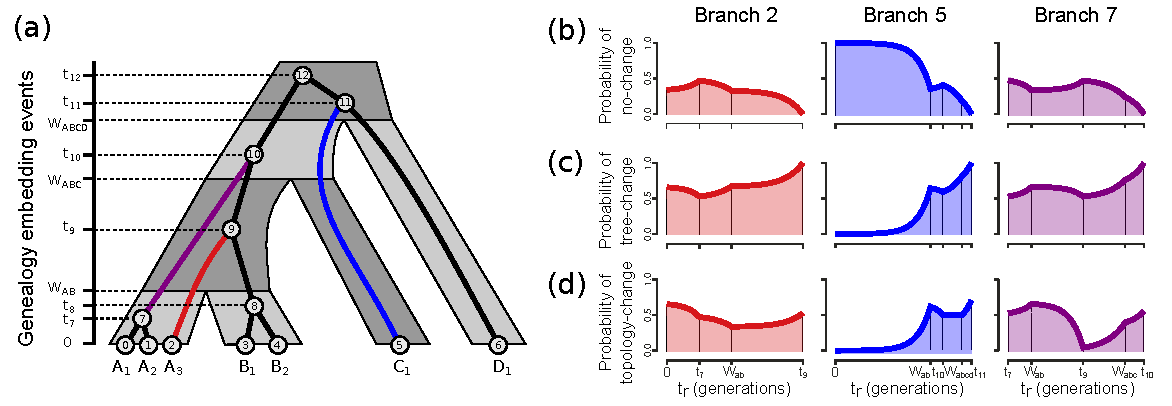
\includegraphics[width=0.99\textwidth]{figures/Fig1-embedding-and-probs-fill.pdf}
	\caption{
		The MS-SMC' models the probability of different outcomes of recombination
		given a genealogy embedded in an multispecies coalescent (MSC) model.
		% The probability of different outcomes of recombination occurring on a 
		% genealogy embedded in a species tree can be modeled using the MS-SMC'. 
		% A genealogy embedded in a species tree exhibits different probabilities
		% of outcomes of recombination, when viewed backwards in time, depending on 
		% the timing and branch on which recombination occurs.
		(a) A parameterized MSC model is composed of multiple discrete population
		intervals with associated effective population sizes ($N_e$) and divergence 
		times ($W$). Given an embedded genealogy, each interval can be further divided 
		at coalescence events (e.g., $t_9$) into a series of smaller intervals
		with constant coalescent rates. The parameters of these intervals make up a 
		genealogy embedding table (see Table 1).
		% varies with respect to
		% changing rates of coalescence, as well the number of samples present at any time.
		% such that the an 
		 % and estimating
		% the expected waiting time between coalescence events (e.g., $t_9$--$t_{10}$) 
		% requires integrating over these rates as they change through time/intervals.
		% See Table 1 for the full genealogy embedding table for this 
		% and the number of samples changes.
		% by the rate of coalescence and the number of samples present.
		% reduce the number of samples present in an interval, whereas population 
		% divergence events (e.g., $W_{AB}$) increase the number in the subsequent interval.
		(b-d) A recombination event leads to one of three possible outcomes 
		between the genealogies in two sequential intervals of a genome: 
		\emph{no-change}, \emph{tree-change}, or \emph{topology-change}. 		
		% "no-change," "tree-change," or "topology-change". 
		% Under the sequentially Markov coalescent (SMC') model a recombination 
		% event will cause one of three possible outcomes between two genealogies 
		% in sequential spatial intervals of a genome: 
		% two sequential intervals
		% can occur on any branch of a genealogy to cause one
		% of three possible outcomes: 
		The probabilities of each outcome as calculated under the MS-SMC' 
		are shown for three branches. These probabilities are a function of the time ($t_r$) and branch 
		on which recombination occurs.
		% Each branch exhibits piecewise variation in these 
		% probabilities across discrete intervals. 
		% % We derive a solution for calculating these probabilities in the text. 
		% Probabilities were calculated here for three selected branches as a 
		% function of the time at which recombination occurs ($t_r$), given the 
		% MSC model in (a) with parameters from Table~S2.% applied to the MSC model in (a).
	% 	divergence times ($W$) define ancestral populations. The population 
	% structure constrains which lineages of the genealogy can coalesce. Further, each 
	% population which can have a different effective population size ($N_b$),
	% which determine rates of coalescence within that population. Viewed backwards in time, 
	% coalescent events (e.g., $t_7$) in the genealogy reduce the number of samples, whereas 
	% species tree divergence events (e.g., $W_{AB}$) increase the number of samples present. 
	% (b-d) 
	% Recombination is modeled by detaching a branch at a specific time and 
	% sampling a waiting time until it re-coalesces, leading to either no change, 
	% a tree change (edge lengths), or topology change. We arbitrarily selected edges 2, 5, and 
	% 7 to illustrate how piecewise variation in coalescent rates back in time through the 
	% species tree leads to changing probabilities of each
	% outcome (discussed in Demonstration). Note that the values in (b) and (c) must sum to 1, 
	% since one of those two events must happen, while (d) is showing the probabilities of a 
	% subset of the events in (c). See Table 1 for the full genealogy embedding table for this 
	% example.
	}
	\label{fig:fig1}
\end{figure}



Importantly, both the coalescent and MSC are models of the expected distribution of 
\emph{unlinked} (uncorrelated) genealogies.
%(non-autocorrelated) genealogies. % sampled from throughout the genome. 
By contrast, two linked genealogies that are drawn from nearby regions of a genome %the genome 
are expected to be more similar than two random draws under these models. This spatial 
autocorrelation is a consequence of shared ancestry among samples at nearby regions, 
which decays over time and distance as recombination events reduce their shared ancestry.
% This process can be approximated by randomly detaching an edge on a genealogy and sampling
% a waiting time (based on the lineage effective population size) until it reconnects
% to the genealogy at a different shared ancestor.
%  % (Fig.~\ref{fig:figS-recomb-types}). # Fig S1 shows the SMC' whereas here we are 
%  % referring simply to the coalescent-with-recomb process.
% In this way, the coalescent with recombination 
% can be viewed as a spatial process 
% where a set of samples at the present substitutes one ancestor for another on 
% either side of a recombination breakpoint \citep{wiuf_recombination_1999}. 
% ADD THIS: \url{https://www.sciencedirect.com/science/article/pii/S0040580914000033}
As a data structure, an ordered series of linked genealogies and the lengths of 
their associated intervals on a chromosome (Fig.~\ref{fig:fig2}) is represented 
by an ancestral recombination graph (ARG)
\citep{griffiths_ancestral_1996}, or similarly, a tree-sequence 
\citep{kelleher2016efficient}
(hereafter we will refer to it generically as an ARG).

% As a data structure, the spatial pattern of linked genealogies spanning
% intervals between recombination breakpoints can be represented either as an 
% ancestral recombination graph (ARG)
% \citep{griffiths_ancestral_1996} or tree-sequence \citep{kelleher2016efficient}
% (hereafter we will refer to it generically as an ARG; Fig.~\ref{fig:fig2}).

An algorithm to stochastically simulate sequences under the coalescent with 
recombination was developed early on \citep{hudson1983properties} 
% , however only with recent advances has it become 
% tractable to scale such simulations to larger, genome-wide scales 
% \citep{kelleher2016efficient}. 
% former new paragraph
% Although it is relatively simple to simulate the coalescent with recombination it has
% proven more challenging to develop an analytical solution for its expected outcome. 
%however it has proven challenging to develop analytical solutions for expected outcomes. 
%This includes 
% the a inference of 
%coalescent times on 
% as a method for stochastically generating ARGs.
% yielding 
% a distribution of linked genealogies associated with intervals
% between recombination breakpoints across a genome.
% and the
% as well as the 
% distribution of 
% brakpoints across the genome where recombination occurred.
% (i.e., "waiting distances").
 % between genealogies).
and was later extended as a spatial algorithm for stochastically generating full 
ARGs \citep{wiuf_recombination_1999}. 
This process models the difference between sequential genealogies by 
randomly detaching an edge from a genealogy and sampling
a waiting time (based on the population coalescent rate) until it reconnects
to the genealogy at a different shared ancestor.
Thus, under this spatial model, a set of samples effectively substitutes
one ancestor for another on either side of each recombination breakpoint.
% Under this spatial model, the coalescent with recombination can thus 
% be viewed as a process where a set of samples at the present substitutes one 
% ancestor for another on either side of a recombination breakpoint 
% \citep{wiuf_recombination_1999}. 
Implicit to this algorithm is the assumption that recombination 
occurs at some predictable rate (or rate map) from which the expected 
waiting distance between recombination events can be modeled as an 
exponentially distributed random variable \citep{wiuf_recombination_1999}.
% (we will refer to ARGs hereafter; Fig. S1).
% While our ability to simulate the coalescent with recombination has made substantial progress, likelihood-based inference of recombination events and coalescent times (that is, the ancestral recombination graph -- "ARG") is notoriously difficult \citep{griffiths_ancestral_1996}. 
% Unfortunately, although 
Although generating ARGs consistent with a demographic model is 
relatively simple under this process, inferring an ARG from sequence data 
-- composing a set of recombination breakpoints and local genealogy inferences -- 
remains highly challenging \citep{y_c_brandt_evaluation_2022}.
This stems in part from the great complexity of this problem 
% and the challenge of distinguishing among many equally probable 
% results given limited information between recombination events;
but also reflects limitations of our current models for 
extracting historical information from linked genome data.

% about linked genealogies.
% infinite series of genealogies can often yield similar
% likelihoods 
% inferring ARGs from sequence data remains challenging, as it is
% computationally intensive, and can be nearly infinite in 
% possibilities for large genome lengths and numbers of samples.
% This stems from the relatively small amount of information 
% This stems mostly from the 
% in part from a relative dearth of models for 
% predicting the similarity of genealogies across different 
% genomic distances.
% or expected
% patterns of genetic linkage across large genomic distances.
% modeling expectations for patterns of genetic linkage across 
% different genomic distances in ARGs remains challenging. 
% linked information in ARGs remains challenging, which in turn limits the 
% amount of information that can be extracted from sequence data for ARG inference. 
% This in turn limits the amount of information that can be extracted from
% sequence data for 
% The problem of inferring ARGs is thus
% computationally intensive, and can be nearly 
% infinite in possibilities for large 
% genome lengths and numbers of samples \citep{mcvean2005approximating}. 
% to perform poorly. 
% have difficulty distinguishing among a nearly infinite range 
% of equally probable results using the limited amount of information 
% present between recombination events. 
% Consequently,
% inferring an ARG from sequence data 
% However, inference of ARGs 
% remains highly challenging, as it 
% is computationally intensive, highly limited by 
% sequence information, and can be nearly infinite in possibilities for large 
% genome lengths and numbers of samples \citep{mcvean2005approximating}. 
% In other words, there
% are usually very few mutations to provide information about each genealogy, 
% and ...
A major advance was achieved through development of the Sequentially Markov 
Coalescent (SMC), a simpler approximation of the coalescent with recombination
that restricts the types of recombination events that can occur 
\citep{mcvean2005approximating}. Specifically,
an edge that is detached from a genealogy by recombination is allowed only to
re-coalesce with ancestral lineages that contributed genetic material to samples
in that interval (as opposed to re-coalescing with any ancestral lineage). 
% the types of coalescent events that can occur between sequential
% space of possible ARGs that 
This greatly reduces the space of possible ARGs without changing the expected
distribution of sequential genealogies, and in doing so it enables modeling
changes between sequential genealogies
as a Markov process \citep{mcvean2005approximating}. 
% This restricts the types of coalescent events that can occur between 
% sequential genealogies, in a way that enables modeling 
% changes between
% models 
% changes among sequential genealogies 
% them 
% Implicit to SMC-based methods is the expectation that recombination occurs at 
% some rate from which the waiting distance between recombination events can be modeled 
% as an exponentially distributed random variable. 
Under these assumptions a tractable likelihood framework can be developed. 
% inferring modeling
% The SMC provides a generative framework for producing a set of genealogies
% and segment lengths under a set of rules 
% The SMC (and related methods) provides a likelihood function 
% for the probability of observing a sequence of genealogies 
% pairwise coalescence times 
% and corresponding segment lengths between them on a genome, 
% given an effective population size and recombination rate. 
% 
% provides a generative framework for genealogies and segment lenghts under 
% a set of rules on which likelihood inference methods can be developed...
% 
% NEXT< start with Because, or something, not however,... 'this is how it is implemented in hmms'
% However, 
Because neither genealogies nor segment lengths can
be observed directly, most SMC-based inference methods use 
% employ 
a hidden Markov model (HMM) to treat these as hidden states 
that influence observable changes in sequence data \citep{spence_inference_2018}.
% be inferred from sequence data. 
% he segment lengths and coalescent times are unknown, most methods use hidden Markov 
% model (HMM) methods in which these are hidden states inferred from sequence 
% data. 
% Further extensions have been developed for modeling variable 
Examples of inference tools built on the SMC framework include 
PSMC \citep{li2011inference} and MSMC \citep{schiffels_inferring_2014}
which use pairwise coalescent times between sequential genealogies
to infer changes in effective population sizes through time, 
and ARGweaver \citep{rasmussen2014genome, hubisz2020inference}, 
which infers ARGs from genome alignments using an SMC-based 
conditional sampling method.
% for inferring changes in effective population sizes
% of single or multiple populations through time, respectively, 
% based on pairwise coalescent times between sequential genealogies;
% % tools for inferring changes in effective population 
% % sizes through time of single (PSMC) or multiple populations (MSMC) 
% % based on pairwise coalescent times \citep{li2011inference, schiffels_inferring_2014}, 
% % , which methods for inferring ARGs using SMC-based conditional 
% % sampling methods
% % based on SMC-like simulations
% %\citep[ARGweaver;][]{rasmussen2014genome, hubisz2020inference}.
% and ARGweaver \citep{rasmussen2014genome, hubisz2020inference}, 
% which infers ARGs from genome alignments using an SMC-based 
% conditional sampling method.

% –- using an approach similar to 
% algorithms for simulating the coalescent with recombination –- 

% However, by modeling the coalescent with recombination
% using a Markovian approximation called the Sequentially Markov Coalescent (SMC), ARG 
% inference becomes more tractable.   
% The SMC is a simplification of the space of possible ARGs -- using an approach similar 
% to the algorithms for simulating the coalescent with recombination -- that models changes
% among sequential genealogies as a Markov process \citep{mcvean2005approximating}.
% IS THIS TECHNICALLY CORRECT?
% \hl{Under the SMC, the likelihood of a sequential set of genealogies and recombination 
% breakpoints (i.e., an ARG) is computed as the product of the set of independent likelihoods
% of observing each change from one genealogy to the next, given an effective population size
% and recombination rate.}
% While explicit likelihood-based inference of ARGs is still difficult, the SMC has enabled 
% \hl{several heuristic approaches to estimating ARGs from sequence data based on inferred 
% recombination events and differences in coalescent times among linked genealogies}
% \citep{li2011inference,rasmussen2014genome,hubisz2020inference}.
% , and the similarities among sequential genealogies, to model
% changes in effective population sizes \citep{}, and to infer 
% ARGs from sequence data 
% historical inferences about changes in effective population sizes, 
% recombination rates, and selection 


% Is this paragraph important? Maybe move to discussion. Concatalescence is not super important to intro.
% Despite the many advances that have been developed for incorporating information 
% from recombination into coalescent inference, the MSC framework (and related 
% fields in phylogenetics, such as the network multispecies coalescent 
% \citep{degnan2018modeling}) continues to largely treat recombination as a source 
% of error as opposed to information.
% This stems from the widely known expectation that, in parts of parameter space, 
% concatenation of sequences from multiple distinct genealogical histories can mislead
% phylogenetic inference. If a concatenated sequence is used to infer a single tree
% representing the species relationships, it might converge on a topology that is different
% from the species tree topology \citep{degnan2006discordance,kubatko2007inconsistency}. 
% The same concatenation biases can affect the distribution of inferred gene trees at
% individual loci as well, with potential effects on species tree or network inference
% methods that take multiple gene trees as inputs -- a process termed "concatalescence"
% \citep{gatesy_concatenation_2013}. The extent to which genetic loci (e.g., exons, UCEs,
% genome windows) represent a single versus multiple genealogical histories can be 
% estimated with coalescent simulations under an MSC model with recombination 
% \citep{mckenzie2020multispecies}. However, analytical solutions have not been
% developed to describe these as distributions within a statistical phylogenetic framework. 


\begin{figure}[t]
	\centering
	%\fbox{\rule[-.5cm]{4cm}{4cm} \rule[-.5cm]{4cm}{0cm}}
	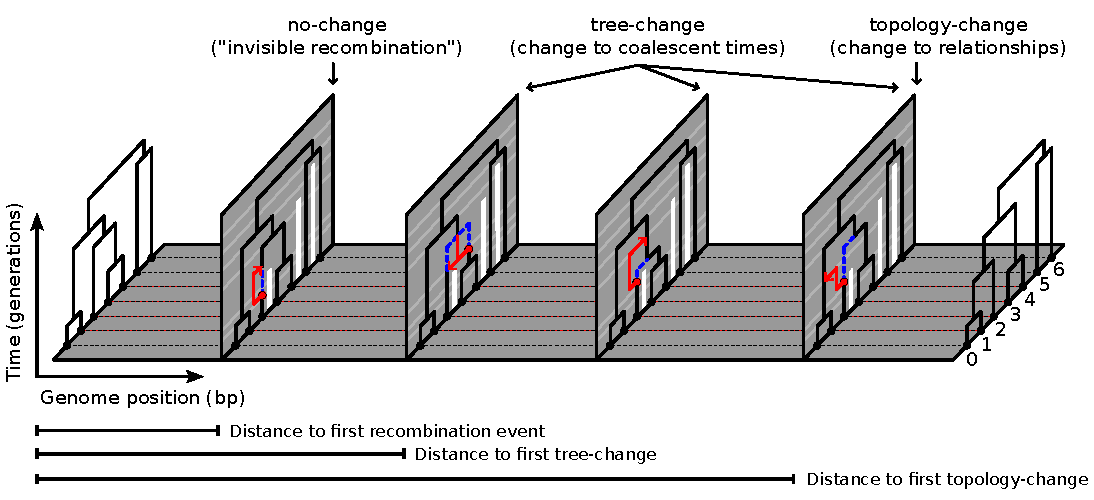
\includegraphics[width=0.99\textwidth]{figures/Fig2-ARG-recomb-types.pdf}
	\caption{
		% An ancestral recombination graph (ARG) with a demonstration of the coalescent
		% with recombination.
		% The MS-SMC' process demonstrated in an ancestral recombination graph (ARG).
		An ancestral recombination graph (ARG)
		is composed of a series of genealogies each spanning non-overlapping 
		intervals of a genome separated by recombination breakpoints. Here, 
		four recombination breakpoints separate the start and end positions 
		on a small chromosome in the history of a set of 7 samples constrained
		by a 4-tip species tree model (as in Fig.~1).
		Recombination events are indicated by vertical panels. Each shows the SMC' process by 
		which a subtree (below the red circle) is detached and then re-coalesces (red arrow)
		with one of the remaining lineages. %, according to the MS-SMC' process. 
		The former edge (blue dotted) which existed throughout the interval to the left of a 
		panel is replaced by a new edge (red) through the subsequent interval. Vertical bars 
		(white) represent barriers to coalescence between samples in different species
		tree intervals (MSC model lineages).
		% ancestor is pruned (blue dotted) 
		% and replaced by a new sampled ancestor (red).
		Four categories of recombination events are shown from left to right, representing
		different outcomes based on the lineage with which a detached subtree re-coalesces.
		% : no-change; tree-change resulting in a shortened coalescence time; 
		% tree-change resulting in a lengthened coalescence time; and tree-change 
		% resulting in a different topology. 
		% These can be further consolidated into 
		These are grouped more generally into 
		three \emph{event types}: (1) no-change, (2) tree-change, and (3) topology-change.
		Every recombination event causes either a no-change or tree-change event, whereas
		a topology-change is a subset of possible tree-change events. The expected waiting
		distance until a specific recombination event type occurs can be calculated under 
		the MS-SMC' given a starting genealogy, MSC model, and recombination rate.
	% Examples of the four different categories of outcomes from a 
	% recombination event (adapted from \citep{deng_distribution_2021}). 
	% (a) A category 1 event occurs when the dislocated lineage reattaches to the 
	% original lineage. 
	% (b) A category 2 event occurs when a dislocated lineage attaches to its 
	% sibling lineage (the lineage that it originally coalesced with), shortening 
	% both of their branch lengths and extending that of its parental lineage. 
	% (c) A category 3 event occurs when the dislocated lineage attaches to its 
	% parental lineage, lengthening the original lineage and its sibling lineage,
	% and shortening the parental lineage.
	% (d) A category 4 recombination event occurs when the dislocated lineage
	% attaches with any lineage other than itself, its sibling lineage, and its
	% parental lineage. This is the only category of recombination event that
	% changes the topology of the genealogy.
}
\label{fig:fig2}
\end{figure}


% Implicit to SMC-based methods is the expectation that recombination occurs at 
% some rate from which the waiting distance between recombination events can be modeled 
% as an exponentially distributed random variable. 
\cite{marjoram2006fast}
described an important extension to the SMC, termed the SMC', for additionally
modeling "invisible" recombination events, in which a detached lineage re-attaches
with its own ancestral lineage prior to the time of that lineage's next coalescent event. 
This leads to no change between the genealogies in two sequential genomic intervals
despite the occurrence of a recombination event between them. The inclusion of
such events has been shown to 
% , such that 
% no change between 
% neighboring genealogies, which has been shown to 
significantly improve inference methods \citep{wilton2015smc}. 
Under the SMC', a detached lineage can thus re-coalesce with an allowable 
ancestral lineage over a continuous range of time, leading to one of 
four possible categorical patterns for the relationship between two
sequential genealogies
% a change 
% relative to the previous genealogy that can be described as one of 
% \hl{four possible categorical} outcomes:
% of possible outcomes of recombination, 
(Fig.~\ref{fig:fig2}, Fig.~\ref{fig:figS-recomb-types}): 
(1) no change %between sequential genealogies;
(2) shortening of a coalescent time; (3) lengthening of a coalescent time; 
and (4) %a coalescent event that changes the topology (relationships). 
a change to the genealogical topology (relationships).
These can be grouped more generally into three types: 
"no-change" (type 1), "tree-change" (types 2-4), and "topology-change"
(type 4). Recently, \citet{deng_distribution_2021} derived a set of solutions for
the expected waiting distances to each of these three types of 
outcomes for a single population with constant effective population size.
% Although all three outcomes, and their associated waiting distances, occur 
% implicitly between sequential genealogies within data generated under the SMC', 
% there was not previously a solution for expectations between events that do 
% not occur sequentially, representing the joint probabilities of multiple events.
% This provides an important advance, for establishing a neutral expectation for 
% turnover 
% in different categorical types of genealogy changes, and for connecting these
% to coalescent model parameters, which may prove useful for future ARG inference 
% tools. 
% 
% 
This provided an important advance by establishing a neutral expectation 
not only for the distance until the next recombination event occurs, 
% 
% but more specifically, for the distance until the next tree-change or 
% topology-change event. Such events leave different detectable signatures 
% in sequence data and extend across larger spatial distances of the genome, 
% thus extending the information content that can be extracted from 
% spatial genealogical patterns.
% 
but more specifically, for the distance until different categorical types
of recombination events occur. Such events leave different detectable 
signatures in sequence data and extend across different spatial distances 
of the genome, thus extending the scale over which information from 
spatial genealogical patterns can be extracted from genomes.
% 
% This provided an important advance by establishing a neutral expectation 
% not only for the distance until the next recombination event occurs, 
% but more specifically, for the distance between different categorical types
% of recombination events that leave different detectable signatures in 
% sequence data. Because such patterns extend over greater spatial distances
% of the genome, they extend the distance over which we can make 
% statistical predictions about spatial genealogical patterns.
% 
% Because they extend over greater spatial distances, information
% from tree-change and topology-change events 
% methods based
% on the detection of
% such patterns can extend the information content of spatial genealogical data.
% until the next tree-change or 
% topology-change event. 
% % Such events leave 
% These different types of recombination events leave different
% detectable signatures in sequence data, and extend across larger 
% spatial distances of the genome, thus extending the information content
% that can be extracted from spatial genealogical patterns.
% than that to the next generic recombination event. 
% This provides an important advance by establishing a neutral expectation 
% not only for the distance until any generic recombination event occurs, 
% but more specifically, for % the different expectations for 
% % for 
% different types 
% of events that leave different detectable signatures in the genome.
% not
% only for any generic recombination events to occur, but for different types 
% of events that leave different detectable signatures in the genome.
% ,which may prove useful for the development of future SMC'-based tools.
% in genealogical topologies, and for connecting coalescent model parameters to these
% outcomes, which may prove useful for future advances in ARG inference. 

% \citep{deng_distribution_2021} recently 
% Their solution assumes a single population with constant effective population size, 
% but nevertheless ... 
% Their solutions 


% recently described a partitioning of different possible outcomes of recombination 
% events into three categories: (1) "no effect", which do not change the genealogy; 
% (2) "tree changes", which affect only coalescent times (edge lengths); and 
% (3) "topology changes", which affect the genealogical relationships.

% the expected waiting distances between
% recombination events, describing different rates for three categorical
% types of recombination events that can occur (Fig.~\ref{fig:fig2}). 
% % 
% This includes recombination events that: (1) have no affect on the 
% genealogical tree; (2) cause "tree changes" (i.e. that they 
% affect either the branch lengths or the topology of the genealogical tree, 
% as in any of categories 2, 3, and 4), and those that cause "topology changes" 
% (only category 4) (\textbf{Figure 1}).


% \citet{deng_distribution_2021} derived an approximate solution for the 
% distribution of waiting distances between sequential genealogies in an ARG. 
% This involved extending the simple expectation for the expected waiting distance
% between *any* recombination event, and partitioning the results into categories
% of different possible outcomes (Fig.~\ref{fig:fig2}). 

% , some of which result in changes to 
% the genealogy, and others of which do not. 
% This represents a major advance. Although 
% The expected waiting distance between any recombination event can be modeled as
% a simple simply described by an exponential distribution}, 
 % under the SMC’ 

% an extension of the SMC that includes "invisible" recombination
% events that result in no change between neighboring genealogical trees. 
% \hl{was known previously}, 
% \citet{deng_distribution_2021} 


Here, we extend the methods of \citet{deng_distribution_2021} to an MSC framework
to estimate the expected waiting distances between different types of 
genealogy changes under a parameterized species tree model. 
The waiting distances between recombination events that cause topology-change 
may be of greatest interest, as they leave the most detectable signatures 
in sequence data and are relevant to expected gene tree distributions that form
an important component of many MSC-based methods \citep{
degnan2006discordance, baum_concordance_2007, knowles_estimating_2011}.
% Just like for single-population models, 
% the waiting distance until a topology-change event in this framework can include multiple
% intervening recombination events of the no-change or tree-change type
The waiting distance between topology-change events may include multiple
intervening recombination events of the no-change or tree-change type
(Fig.~\ref{fig:fig2}). 
The relative occurrence of events that do not result in topology 
changes can be especially high in small sample sizes \citep{wilton2015smc}, 
which are common in MSC-type datasets in which samples are partitioned 
among species tree intervals. 
% The partitioning of 
% recombination events that of categories 1-3 occur 
% disproportionately often in small sample sizes \citep{wilton2015smc}, 
% which are especially common in MSC-type datasets since
% samples are partitioned among species tree intervals. 
Since the partitioning of 
coalescent events among species tree intervals is expected to constrain 
the types of recombination events that will be observed, the
distributions of waiting distances between different types of 
genealogy changes should be highly dependent on, and thus informative about, 
the species tree model. We refer to the general framework of embedding the 
SMC' in an MSC model as the MS-SMC'.


% The relative frequency
% of different event types is therefore expected to be contingent on parameters
% of the species tree. 

% Recombination events of type 4 are of greatest interest
% % the most inherently interesting 
% for most applications,
% % because s
% as they leave the most detectable signal in sequence data.
% % since they will produce the most obvious signal in the sequence data. 
% However, events of types 1-3 occur disproportionately often in small sample 
% sizes \citep{wilton2015smc}, which are especially common in MSC-based studies, 
% where genealogies are embedded within a species tree, such that fewer samples 
% typically represent each lineage. But the
% relative frequency of the different events is contingent upon the Ne values of the
% species tree branches and on the species divergence times. In other words, the 
% partitioning of coalescence events among lineages of the species tree topology is
% expected to constrain the types of recombination events that are more likely to be
% observed. This results in distributions of waiting distances between genealogical
% changes being highly dependent upon parameters of the species tree model. 

% With this in mind, we extend the method of \citet{deng_distribution_2021} to the MSC
% to predict the expected waiting distances between genealogy changes under a 
% parameterized species tree model. This new solution is important for establishing an 
% expectation for the neutral rate of genealogy turnover under different species tree 
% parameterizations. It may also have applications for ARG inference under complex 
% demographic models \citep[e.g.,][]{hubisz2020mapping}, potentially serving as a 
% component of a likelihood function for inferring species trees from linked 
% genealogies -- a future theoretical goal.

% MS-SMC: multispecies sequentially markovian coalescent
% SM-MSC: sequentially markovian multispecies coalescent

%Solutions exist for simulating genomes under the coalescent with recombination \citet{ipcoal, kelleher, hudson}. In particular, \emph{msprime} is a powerful and flexible tool for simulating ancestral recombination graphs for many samples under user-defined demographic scenarios. \emph{ipcoal} is an extension of msprime that accepts multispecies coalescent parameters. 

%Phylogenetic methods sampling regions throughout the genome have increasingly adopted the multispecies coalescent model to incorporate variation in regions due to incomplete lineage sorting. Applications of the multispecies coalescent in phylogenetic inference aim to avoid known bias under which, in certain circumstances, phylogenies inferred from concatenated data might converge on a tree that is not the species tree. One challenge of applying the multispecies coalescent for species tree inference is properly defining the breakpoints for loci used in the analysis. Often this is done arbitrarily: researchers ensure that loci are long enough to infer reliable gene trees, and that there are enough inferred gene trees to infer a robust species tree. However, there has been some debate in the literature over the effects of locus length on species tree inference. Specifically,  

%Another way in which the ancestral recombination graph is relevant to phylogeneticists is for local inference...

%Recently, \citet{deng_distribution_2021} provided a solution for the distribution of waiting times to genealogical changes under the SMC', a popular model for simulating ancestral recombination graphs. However, their solution is constrained to a single population of constant effective population size.

%Establishing the predicted length of different topologies along the chromosome is important for inference of local genealogies in population genetics, which can be used for inference of selection, demographic changes, and introgression. It is also important in multispecies coalescent methods in phylogenetics, which often rely on inference of gene trees.


% springer + gatesy

% inference, argweaver-D



%%%%%%%%%%%%%%%%%%%%%%%%%%%%%%%%%%%%%%%%%%%%%%%%%%%%%%%%%%%%%%%%%%%%%%%%%%%
%%%%%%%%%%%%%%%%%%%%%%%%%%%%%%%%%%%%%%%%%%%%%%%%%%%%%%%%%%%%%%%%%%%%%%%%%%%
%%%%%%%%%%%%%%%%%%%%%%%%%%%%%%%%%%%%%%%%%%%%%%%%%%%%%%%%%%%%%%%%%%%%%%%%%%%
%%%%%%%%%%%%%%%%%%%%%%%%%%%%%%%%%%%%%%%%%%%%%%%%%%%%%%%%%%%%%%%%%%%%%%%%%%%
%%%%%%%%%%%%%%%%%%%%%%%%%%%%%%%%%%%%%%%%%%%%%%%%%%%%%%%%%%%%%%%%%%%%%%%%%%%
%%%%%%%%%%%%%%%%%%%%%%%%%%%%%%%%%%%%%%%%%%%%%%%%%%%%%%%%%%%%%%%%%%%%%%%%%%%
%%%%%%%%%%%%%%%%%%%%%%%%%%%%%%%%%%%%%%%%%%%%%%%%%%%%%%%%%%%%%%%%%%%%%%%%%%%
%%%%%%%%%%%%%%%%%%%%%%%%%%%%%%%%%%%%%%%%%%%%%%%%%%%%%%%%%%%%%%%%%%%%%%%%%%%
%%%%%%%%%%%%%%%%%%%%%%%%%%%%%%%%%%%%%%%%%%%%%%%%%%%%%%%%%%%%%%%%%%%%%%%%%%%
%%%%%%%%%%%%%%%%%%%%%%%%%%%%%%%%%%%%%%%%%%%%%%%%%%%%%%%%%%%%%%%%%%%%%%%%%%%






\section{Approach}
\subsection{Comparison to Deng \emph{et al.} (2021)} %\citet{deng_distribution_2021}}

Our approach is a generalization of the \citet{deng_distribution_2021} derivation 
of waiting distances to genealogy changes for a single population of constant size. 
We modified the single-population model to (1) include barriers to coalescence imposed
by a species tree topology, and (2) integrate over changing coalescence rates along
paths through multiple species tree intervals with different effective population 
sizes. In addition, we have implemented a novel likelihood framework for inferring 
parameters of an MSC model from observed waiting distances between genealogies.
% We have intentionally reproduced our equations in a similar structure and using
% many of the same variable names as in \citet{deng_distribution_2021}.
% to highlight the changes we made to generalize their solution.


\subsection{MSC model description}
% We assume a species tree model with divergence times in units of generations and 
Given an MSC model ($\mathcal{S}$) composed of a species tree topology with divergence
times ($W$) in units of generations and constant diploid effective population 
sizes ($N_e$) assigned to each branch, an embedded genealogy ($\mathcal{G}$) for 
any number of sampled gene copies ($k$) can be generated
by randomly sampling coalescent times at which to join two samples into a 
common ancestor, starting from samples at the present in each interval.
% 
% . This is accomplished by randomly sampling coalescent times 
% at which to join two samples into a common ancestor, 
% starting from samples at the present in each interval. 
% 
% 'in each interval' is to be clear that we move piecewise through the MSC model.
% 
Following \citet{kingman1982coalescent}, the probability of a 
coalescent event one generation in the past (reducing the 
number of samples from $k$ to $k$-1) %in a single population
is given by equation 1. From this, we can model the expected 
waiting time ($\mathbb{E}[t_k]$) until the next coalescence event as an 
exponentially distributed random variable with rate parameter $\lambda_k$:

\begin{equation}
\begin{aligned}
	&\lambda_k = \mathbb{P}(\text{coal~event~} | N_e,k) = \frac{k(k-1)}{2N_e}
	\\
	&~~and:
	\\[0.15cm]
	&\mathbb{E}[t_k] = 1 / \lambda_k
	\\[0.15cm]	
\end{aligned}
\end{equation}

\noindent In a single population model
with constant $N_e$ the expected waiting time between coalescent events 
increases monotonically after each coalescent event, since the number of
% with constant $N_e$, the expected waiting time between coalescent events 
% increases monotonically after each coalescent event. This is because the number of 
remaining samples always decreases. In an MSC model, 
however, the expected waiting time between coalescence events can increase or 
decrease through time, as the transition from one population interval to another 
can be associated with a different $N_e$ value and an increase in the number 
of samples.
% to the next can be 
% associated with different N$_b$, and because the merging of samples from 
% number of samples increases
% in ancestral population intervals when descendant branch intervals are merged.

Based on this generative framework for sampling genealogies, likelihood
solutions have been developed to fit coalescent model parameters, such as 
$N_e$ in single population models \citep{kingman1982coalescent},
or multiple $N_e$ and $W$ parameters in MSC models \citep{rannala2003bayes}, 
based on inferred coalescence times. 
In the latter framework, each species tree branch interval is treated independently, 
such that the likelihood of a genealogy embedding is calculated from the joint
probability of observing each distribution of coalescent waiting times within
each species tree branch interval. A key feature of these equations is that 
when $k$ lineages are present, we can use the coalescent rate parameters 
($\lambda_k$)
% \hl{the inverse of} equation 1 as a rate parameter ($\lambda$)
to calculate the likelihood of observed waiting times between coalescent 
events ($t_k$) in each population interval from an exponential probability 
density function:
% for the expected rate
% of coalescence
% between when $k$ and $k$ - 1 lineages exist. 
%  and thus the probability of 
% when Using the expected time between coalescence
% events when $k$ lineages are present (equation 1) as a rate parameter, the 
% likelihood of an observed waiting time can be calculated from an exponential 
% probability density. 
	
\begin{equation}
	% \mathcal{P}(t_k|\lambda) = \lambda e^{-\lambda t_k} 
	f(t_k; \lambda) = \lambda e^{-\lambda t_k}
\end{equation}


% In each species tree interval this is repeated for each interval between 
% observed coalescent events.

% The probability of a particular genealogical topology among a set of coalesced
% samples in an interval. The probability a particular pair of lineages coalesce
% is 1 ( kchoose2) = (2 / (j * (j - 1))), where j=m, n, n+1. [Describe m and n as
% the start and end of intervals.]

% \begin{equation}
% 	\mathbb{P}(t_k | N_e) = 
% 		\frac{1}{2N_e} 
% 		\exp \bigg\{-\frac{k(k-1)}{4N_e} t_k \bigg\} \times 
% 		\exp \bigg\{-\frac{n(n-1)}{4N_e} (\tau - (t_m + t_{m-1} + \text{...} + t_{m+1})) \bigg\}
% \end{equation}

% Similarly, the likelihood of observing a set of coalescent
% times on a genealogy embedded in a species tree can be calculated from the
% joint probability of its observed coalescence times within each interval
% \citep{rannala2003bayes}, treating intervals independently. 
% Thus, the genealogy (G) in Figure 1 can be calculated as
% ...

% Generating unlinked genealogical trees under the MSC is straightforward: Coalescent events between samples can only happen after (moving backward in time) coalescence of the species that contain them, and the coalescent rate in each part of the tree is dependent on both the number of genealogical lineages that can coalesce in that section and on the effective population size in that section.

\subsection{MS-SMC' model description and notation}

% Under the single-population SMC' 
% considered by \citet{deng_distribution_2021}, the 
Under the SMC' model, sampling of a linked genealogy requires considering not only 
%a species tree and its parameters, 
demographic model parameters, 
as we did above, but also an existing genealogy -- it is a method 
for sampling the next genealogy conditional on the previously observed one. 
If we define the previous genealogy as $\mathcal{G}$, and the sum of its edge lengths 
as $L(\mathcal{G})$, then under the assumption of a constant recombination rate through time,
a recombination break point can be uniformly sampled from $L(\mathcal{G})$ to occur with 
equal probability anywhere on $\mathcal{G}$. 
% on any branch.
A recombination event creates a bisection on a branch, separating a subtree 
below the cut from the rest of the genealogy 
(Fig.~\ref{fig:fig2}, Fig.~\ref{fig:figS-recomb-types}).
% (Fig.~\ref{fig:fig2}). 
The subtree must then re-coalesce 
with an edge on the genealogy from which it was detached at a time
above the recombination event.
%in the to connect with one of the edges of %remaining edges on 
% the genealogy at a time above the recombination event. 
The waiting time until 
this re-coalescence event occurs is sampled stochastically with an expectation 
determined by the number of samples and the coalescent rate, 
similar to equation 1.
% the expected waiting time as until re-coalescence the 
% same as described above (equations 1 and 2).

In a single population model with constant $N_e$ the expected waiting time until 
re-coalescence increases monotonically with each coalescence event 
backwards in time, since each event decreases $k$.
% (e.g., Fig.~1B). 
Once again, the MSC model differs from this: 
coalescent events similarly decrease $k$, but the merging of 
species tree branches into ancestral intervals increases $k$, and $N_e$ 
can also vary among species tree intervals. 
Thus, the probability that a detached subtree re-coalesces to the genealogy 
can vary through time along its path of possible reconnection points through 
different species tree intervals
(Fig.~\ref{fig:fig1}b-d).
To calculate these probabilities, a species tree can be decomposed into a 
series of relevant intervals between events that change rates of coalescence,
% , including within species tree intervals, 
which we refer to as the genealogy embedding table (Table~\ref{tab:table-1}). 
From this table it is possible to calculate the probabilities of different
recombination event type outcomes, and consequently, to model the expected 
waiting distances until specific recombination event types occur. 

% Using this information on the rate of coalescence within each genealogy
% embedding interval, it is then possible to model the probability that a
% detached lineage will re-coalesce within any specific interval. From this, 
% it is then possible to calculate probabilities of different recombination event types which 
% are a
% Our goal ... The goal of the MS... To model the probabilities of different
% genealogy change events we must model the probability that a detached lineage
% will re-coalesce with any allowed ancestral lineage while constrained by the
% MSC model. This requires integrating over the coalescence rates which can 
% vary among intervals of the species tree model.


\begin{table}[t]
\centering
\caption{
	A genealogy embedding table for the genealogy and species tree in Figure 1. 
	The probability of coalescence is constant within each discrete interval 
	and is scaled by the number of lineages ($k$), the effective population size ($n$), 
	and the interval length ($d$).
	% present ($k$) and the effective population size ($N_e$). 
	Under the MS-SMC', the probability that a detached lineage will re-coalesce
	on a specific branch of the genealogy (e.g., branch 7 from Figure~\ref{fig:fig1})
	is calculated from the piecewise constant probabilities in each 
	discrete interval spanning that branch (e.g., rows 1, 6, 7, and 8).
}
\begin{tabular}[t]{ |c|c|c|c|c|c|c|c|c| }
	\toprule
	 % & start ($t_i^l$)  & end ($t_i^u$) 
	 & start ($\sigma$)  & end ($\mu$)  & pop & $N_e$ ($n$)  & N edges ($k$) & coal  & length ($d$) & branches ($b$) \\
	\midrule
	0 & 0          & $t_7$      & A   & $N_A$     & 3 & $t_7$    & $t_7$ - 0            & 0,1,2 \\
	1 & $t_7$      & $W_{AB}$   & A   & $N_A$     & 2 & -        & $W_{AB}$ - $t_7$     & 2,7   \\	
	2 & 0          & $t_8$      & B   & $N_B$     & 2 & $t_8$    & $t_8$ - 0            & 3,4   \\ 
	3 & $t_8$      & $W_{AB}$   & B   & $N_B$     & 1 & -        & $W_{AB}$ - $t_8$     & 8     \\
	4 & 0          & $W_{ABC}$  & C   & $N_C$     & 1 & -        & $W_{ABC}$            & 5     \\
	5 & 0          & $W_{ABCD}$ & D   & $N_D$     & 1 & -        & $W_{ABCD}$           & 6     \\
	% 
	6 & $W_{AB}$   & $t_9$      & AB  & $N_{AB}$  & 3 & $t_9$    & $t_9$ - $W_{AB}$     & 2,7,8 \\
	7 & $t_9$      & $W_{ABC}$  & AB  & $N_{AB}$  & 2 & -        & $W_{ABC}$ - $t_9$    & 7,9   \\
	% 
	8 & $W_{ABC}$  & $t_{10}$   & ABC & $N_{ABC}$ & 3 & $t_{10}$ & $t_{10}$ - $W_{ABC}$ & 5,7,9  \\
	9 & $t_{10}$   & $W_{ABCD}$ & ABC & $N_{ABC}$ & 2 & -        & $W_{ABCD}$ - $t_{10}$ & 5,10 \\
	%
	10 & $W_{ABCD}$ & $t_{11}$  & ABCD & $N_{ABCD}$ & 3 & $t_{11}$ & $t_{11}$ - $W_{ABCD}$ & 5,6,10 \\
	11 & $t_{11}$  & $t_{12}$   & ABCD & $N_{ABCD}$ & 2 & $t_{12}$ & $t_{12}$ - $t_{11}$ & 10,11 \\
	12 & $t_{12}$  & -          & ABCD & $N_{ABCD}$ & 1 & -        & -                   & 12    \\	
	\bottomrule
\end{tabular}
\label{tab:table-1} 
\end{table}

Each interval of the genealogy embedding table contains a constant number
of genealogy branches ($k_i$) and a constant effective population size 
($n_i$) such that the rate of coalescence is also constant.
We define a number of additional variables related to this table. 
The length of each interval is $d_i$, and its lower and upper bounds 
are $\sigma_i$ and $\mu_i$, respectively. Similarly, the lower and upper 
bounds of a genealogy branch ($b$) are defined as $t_b^l$ and $t_b^u$, 
respectively. 
% Each interval has a constant 
% number of genealogy branches $k_i$, and effective population size $n_i$.
An indexing variable, $\mathcal{I}_b$, is defined as the
ordered set of intervals that are spanned by a specific branch
of an embedded genealogy. As an example, consider branch 7 from 
Fig.~\ref{fig:fig1}. This branch spans four intervals, 
labeled as rows 1, 6, 7, and 8 in Table~\ref{tab:table-1}, 
and so $\mathcal{I}_7$ = \{1,6,7,8\}. As we will
demonstrate below, this and related indexing variables will be
used to calculate the probabilities of re-coalescence in different
intervals, and on different branches, based on their rates of 
coalescence.
A summary of all variables in our notation is available in 
table~\ref{tab:table-notation}. 

% To better understand the relationship between the MS-SMC' and the genealogy
% embedding table, consider a specific branch ($b$) from Fig.~\ref{fig:fig1}. 
% Branch 7 on the genealogy spans four relevant intervals, 
% labeled as rows 1, 6, 7, and 8 in Table~\ref{tab:table-1}.
% This ordered set is defined as $\mathcal{I}_b$, such that, for example, 
% $\mathcal{I}_7$ = \{1,6,7,8\}. 
% Several additional indexing variables are described below;
% a summary of all variables is available in table~\ref{tab:table-notation}). 

% The coalescent rate within each interval can be calculated from its
% \hl{diploid} effective population size ($n_i$) and number of samples 
% present ($a_i$). 
% The lower and upper bounds of each interval are defined as 
% $\sigma_i$ and $\mu_i$, respectively, and its length as $d_i$. 
% Similarly, the lower and upper bounds of each branch are defined 
% as $t_b^l$ and $t_b^u$, respectively. Each interval has a constant 
% number of genealogy branches $k_i$, and effective population size $n_i$.
% This is used in the equations below as an
% index to iterate over the ordered sequence of intervals on a branch. 
% By iterating over all $i$ intervals from 0 to $\mathcal{I}_b - 1$ 
% different rates can be applied to different intervals over the length 
% of a branch.
% (this can be found by searching for the branch label in the \emph{branches} 
% column of the table). 
% We record the number 
% of intervals in which a branch is present as $\mathcal{I}_b$, such that,
% for example, $\mathcal{I}_7$=4. We use this indexing variable to iterate
% over the ordered sequence of intervals on a branch. 
% over the lengths of each interval on a branch. 
% The coalescent rate within each genealogy embedding interval of the
% table is calculated from the \hl{diploid} effective population size ($n_i$) 
% and number of samples present ($a_i$).
% to the end of the last interval $\sigma_{\mathcal{I}_{b+1}}$.
% For this branch, we are interested in defining intervals where 
% coalescent rate parameters change, 
% which involves identifying coalescent events that occur in the same species
% tree intervals as this branch, as well as events where this branch 
% transitions from one species tree interval to the next.
% To do so, we must identify times at which there are relevant coalescent events 
% between other lineages in the same population, or at which there are relevant 
% species merging events. 
% This involves examining the genealogical tree as it is 
% embedded within the species tree. With the genealogy embedding table, we can 
% In the genealogy embedding table we can then query the "branch" column to
% isolate intervals involving branch 7. This corresponds to rows 1, 6, 7, and 8, 
% such that the number of intervals on branch 7 ($\mathcal{I}_b$) is four. 
% The time of the start of each interval ($i$) is $\sigma_i$. 
% \hl{An integer index ($\mathcal{I}$) stores the number of intervals that 
% each branch occurs in, such that enumerating over the range
% of $\mathcal{I}_b$ visits each interval in order along 
% genealogy branch $b$.} 
% easily isolate the intervals specific to edge 7 by querying the "branches" 
% column of the table and extracting the rows where this column contains our 
% focal edge (for edge 7, these are rows 1, 6, 7, and 8). 
% The number of rows is equal to the 
% The number of rows 
% we extract (in this case, 4) is equal to the number of intervals in the edge 
% ($\mathcal{I}_b$). If we retain the relative order of the rows and re-index them from 
% $0$ to $\mathcal{I}_b-1$, the information in the columns (e.g. $n_i$, $a_i$) is easily
% adapted for use in the equations presented below. 
% Each branch of $\mathcal{G}$ spans one or more intervals
% from which a lower and upper (min, max) bound for that branch can also be 
% extracted ($t_b^l$ and $t_b^u$, respectively). 
% Later, we describe equations that require information about how genealogy branches are 
% related (e.g., parent-child or siblings), which can also be extracted from $\mathcal{G}$
% and represented as a table. 
% Some additional indexing variables are also described below;
% a summary of all variables is available in table~\ref{tab:table-notation}). 

% This and the genealogy embedding table include all
% relevant parameters for the equations below. 
 % \hl{(e.g., Table~S1).}
% . For example, 
% edge 2 from Fig.~\ref{fig:fig1} and Table~\ref{tab:table-1} overlaps with 
% three intervals, such that $\mathcal{I}_2$ = 3.
% \hl{From this gene tree embedding we also define 
% the set $\mathcal{I}$ that includes the indices of all intervals in the table. 
% And we define an indexing variable $I_b$ for each branch ($b$) in $\mathcal{G}$ that
% returns a vector of ordered intervals ($i \in \mathcal{I}$) that overlap with 
% a specific gene tree branch.}
% For example, edge 2 from Fig.~\ref{fig:fig1} and Table~\ref{tab:table-1} overlaps with 
% three intervals, such that $I_2$ = (0, 1, 6). 
% These variables, and the genealogy embedding table, 
% together include all relevant parameters for the derivations below. 



% To summarize, the genealogy embedding table is simply a set containing all 
% unique intervals (and their properties) over all edges in the genealogy, 
% and it maps those intervals to the genealogy edges to which they belong. 
% This allows us to easily query relevant intervals for any edge of the 
% genealogical tree. For extracting relationships among branches (e.g. parent,
% sibling, as required for the topology cahnge equations), we can reference a 
% separate table specific to the structure of the genealogical tree only (see 
% Appendix, Table 2).
% , and are also summarized in the Appendix.

%\hl{needs updates to figure out how table can align with existing variables names.
%Additional table with final info could be supplement. Includes I, sister index, parent index...}

% Unlike in the single-population SMC', the intervals in the multispecies model
% are branch-specific. For example, the breakpoint $\sigma_{D1}$ in Figure 2c  
% corresponds to the species tree coalescence of species C and species D. This 
% increases the number of lineages available for the D lineage to coalesce with 
% (from 1 -- itself -- to 2) and might also change the effective population size.
% However, this breakpoint does not appear in Figure 2d since the lineage in species
% E is not able to coalesce with lineages from species C or D until $\sigma_{E1}$,
% when E coalesces with the ancestor of C and D in the species tree.




% In the MS-SMC', we specify a model with piecewise-constant coalescence rates. 
% However, intervals under the MSC adaptation are bounded not just by coalescence
% events in the \emph{genealogy} tree (decreasing the number of available lineages for 
% coalescence), but also by relevant coalescences in the \emph{species} tree. Species 
% coalesence events increase the number of genealogical lineages available for 
% coalescence, and they also can correspond to changes in effective population 
% size (\textbf{Figure 2}). 

% Having described our model, we also adopt the following notation:

% \begin{itemize}
%   \item $\mathcal{I}_b$: index of an interval on genealogy branch $b$. A genealogy 
%   branch is split into discrete intervals corresponding to points along its length 
%   at which either the species tree interval changes, or the number of samples $k$ with
%   which it can coalesce changes.
%   \item $t^u_b$: the height, in generations, of the upper bound of genealogy branch $b$.
%   \item $t^l_b$: the height, in generations, of the lower bound of genealogy branch $b$.
%   \item $\mathcal{T}$: the genealogical tree
%   \item $\mathcal{S}$: the species tree
%   \item $\mathcal{N}$: the number of tips in the species tree
%   \item $L(\mathcal{T})$: the total genealogical tree length, in generations
%   \item All summations where the stopping value is less than the starting value are equal to zero.
% \end{itemize}

% Several values are indicated only on one branch at a time, and thus we do not include 
% an underscore to indicate which branch. These are:
% \begin{itemize}
%   \item $\sigma_i$: the length, in generations, of the lower bound of interval $i$ on branch $b$.
%   \item $n_i$: the effective population size of species tree interval index $i$.
%   \item $a_i$: the number of available lineages to coalesce with in the genealogy interval with index $i$.
%   \item $T_i$: the length, in generations, of species tree interval with index $i$.
% \end{itemize}


\subsection{Deriving probabilities of genealogy changes in the MS-SMC'}
A recombination event occurring on $\mathcal{G}$ can result 
in three types of outcomes (Fig.~\ref{fig:fig2}).
Of these, there is a zero-sum relationship between a no-change and 
tree-change event, such that one or the other must occur.
% one or the other must always occur.
% , resulting in either 
% no change to the genealogy, a change only to its branch lengths, 
% or a change to its topology. 
Therefore, as a first step towards describing probability statements 
for each of these event types, we focus first on deriving the 
probability of a no-change event 
(also termed a tree-unchanged event; Fig.~\ref{fig:fig3}a), 
which is the simplest outcome. Then, from the law of total probability, 
we also have a result for the probability of recombination resulting in 
a tree-change event. 
% From this, we can then calculate the probability of a tree-change
% by the law of total probability. 
% Therefore, our first step in deriving probability statements for
% Our first step in deriving probability statements for
% these different outcomes is to calculate the probability of a no-change event. 
Finally, to calculate the probability of a topology-change event, 
we first derive a statement for the probability of a topology-unchanged event
(Fig.~\ref{fig:fig3}d), which is the union of a no-change event and
a subset of tree-change events,
where the detached lineage is restricted according to which ancestral lineages 
it can re-coalesce with. 
Full detailed derivations of all solutions below are available in the 
Appendix of the Supplementary Materials.
% we calculate the probability of topology-change as a subset of
% the probability of a tree-change, in which we restrict which branches the
% detached lineage can re-coalesce with.
% events. 
% probabilities 
% of events that 
% fall into the other categories.
% In category 1, there is no change to the genealogy. In categories 2 and 3 only
% a the branch lengths of the genealogical tree change while the topology remains
% the same. In category 4, the topology of the resulting tree is different from the 
% original tree. For simplicity, we will refer to changes that affect only branch
% lengths (categories 2-3) as those that change \emph{the tree}, and category 4 as 
% those that change \emph{the topology}.
% Our first steps are to calculate the probability of a recombination event in
% category 1, where the new genealogical tree is identical to the previous tree. The 
% law of total probability then allows us to use the inverse probability to calculate
% a waiting distance to a change that falls into any of categories 2, 3, or 4. 


\subsubsection{Probability of a no-change event}
% \subsubsection{Probability that a recombination event at time $t$ on branch $b$ will not change the tree:}
% \hl{these sections needs waay more description. What does this all mean? The text here
% was only restating the section title. You need to build up to the more complex ones by 
% walking the readers through the more simple examples. I think this is super important
% to make this work understandable. Think of Rannala and Yang 2003.}
We begin by assuming knowledge of when and where recombination takes place, in terms 
of a recombination event bisecting branch $b$ at time $t_r$. %The variable $\sigma$ 
% The index $i$ refers to the genealogy embedding interval in which recombination occurs.
For no change to occur to the genealogy, the detached subtree must re-coalesce with 
its original branch -- either in the same interval from which it detached, or in a
later interval on the same branch (Fig.~\ref{fig:fig3}a). %during the same interval in which it detached.
If it connects to any other lineage this will cause a change to either the tree 
or topology. 
Equation 3 describes the probability of a no-change event 
given a genealogy embedded in a species tree, and the timing and branch on 
which recombination occurs. The interval in which recombination occurs 
% at time $t_r$ on branch $b$ 
is labeled $i$. 
The first two terms describe the probability that the subtree re-coalesces 
during interval $i$ on branch $b$ (i.e., $ii$), 
while the latter term is the probability of re-coalescing
during a later interval on branch $b$ (i.e., $ij$). For this, we define 
another indexing variable $\mathcal{J}_b(i)$ = $\{j \in \mathcal{I}_b ~|~ j > i\}$, 
for iterating over the ordered intervals above $i$ on branch $b$ (e.g., Fig.~\ref{fig:fig3}b).
% and does not re-coalesce with any other lineages during this interval. The
% later term describes a sum over all subsequent intervals on $b$, 
% the probability that this subtree coalesces with its originating 
% branch in a later interval (i.e., $ij$), and does not re-coalesce with any other 
% lineages in a later interval.%on this same branch. 

\begin{figure}[t]
	\centering
	\includegraphics[width=0.99\textwidth]{figures/interval-functions}
	\caption{
		% Rates of coalescence are piece-wise constant within discrete intervals 
		% of the genealogy embedding table. 
		The probabilities of different recombination event types are calculated from 
		piece-wise constant probabilities of recombination within discrete intervals.
		% probability statements for recombination occurring
		% at time $t_r$ in interval $i$ and re-coalescing in interval $j$. 
		(a) The probability of a no-change event involves re-coalescing on the same 
		branch on which recombination occurred, for which intervals are indexed using
		the variable $\mathcal{I}_b$.
		%, or $\mathcal{J}_b(i)$. 
		(c,f) The function $f(i,j)$ returns the probability that a subtree detached 
		in interval $i$ will re-coalesce in interval $j$. This involves excluding
		the probability of re-coalescence in intervals between $i$ and $j$, which is 
		indexed as $\mathcal{Q}_b(i,j)$. 
		(d) The probability of a topology-unchanged event involves re-coalescing on the 
		same branch on which recombination occurred, or its parent or sibling branches. 
		(e) Additional indexing variables return intervals on the parent branch 
		($\mathcal{I}_c$), or the sibling branch above ($\mathcal{M}_b$) or below 
		($\mathcal{L}_b$) the time at which it overlaps in the same species tree interval
		as branch $b$, termed $t_b^m$.
	}
	\label{fig:fig3}
\end{figure}


% PREVIOUS APPROVED EQUATION 3
\begin{equation}
\begin{aligned}
	&\mathbb{P}(\text{no-change} | \mathcal{S},\mathcal{G},b,t_r) = 
	\frac{1}{k_i} + 
	f(i,i) \exp \bigg\{ \frac{k_i}{2n_i} t_r \bigg\} +
	\sum_{j \in \mathcal{J}_b(i)} f(i,j) \exp \bigg\{ \frac{k_i}{2n_i} t_r\bigg\}
	% \sum_{j=i+1}^{\mathcal{I}_b - 1} f(i,j) \exp\bigg\{\frac{a_i}{2n_i}t_r\bigg\} 
\end{aligned}
\end{equation}


\noindent This equation is simplified by use of the function $f(i,j)$
to return the piece-wise constant probabilities of re-coalescence between
pairs of intervals. When $j=i$, this expression involves the probability of 
coalescing over the remaining length of interval $i$ above $t_r$; 
when $j>i$ it involves the probability of coalescing in interval 
$j$ and not coalescing in interval $i$ or any other intervals 
between $i$ and $j$. For this latter process, we define another
indexing variable, $\mathcal{Q}_b(i,j)$ = $\{q \in \mathcal{I}_b ~|~ j > q > i\}$, 
for iterating over the ordered intervals above $i$ and below $j$ 
on branch $b$ (e.g., Fig.~\ref{fig:fig3}c).
The function $f(i,j)$ forms the core of the MS-SMC' algorithm, and 
will reappear in several later equations.

\begin{equation}
\begin{aligned}	
	f(i,j) = 
	\begin{dcases}
		- \frac{1}{k_i} \exp \bigg\{-\frac{k_i}{2n_i}\mu_i \bigg\}, 
		& \text{if } i=j\\
		% 
		\frac{1}{k_j} \left(1 - \exp \bigg\{ -\frac{k_j}{2n_j} d_j \bigg\} 
		\right)
		\exp \bigg\{ -\frac{k_i}{2n_i}\mu_i - 
		\sum_{q \in \mathcal{Q}_b(i,j)} \frac{k_q}{2n_q} d_q \bigg \}, 
		& \text{if } i\ne j\\
	\end{dcases}
\end{aligned}
\end{equation}

% PREVIOUS APPROVED EQUATION 4
% \begin{equation}
% \begin{aligned}
% 	% &P_{ii} = - \frac{1}{a_i} \exp \bigg\{-\frac{a_i}{n_i}(t_i^u - t_r) \bigg\} 
% 	&P_{ii} = - \frac{1}{a_i} \exp \bigg\{-\frac{a_i}{n_i}\sigma_{i + 1} \bigg\} 	
% \end{aligned}
% \end{equation}

% \begin{equation}
% \begin{aligned}
% 	&P_{ij} = 
% 	\left( \frac{1}{a_j} (1 - \exp \bigg\{ -\frac{a_j}{n_j} d_j \bigg\} \right)
% 	\times
% 	\exp \bigg\{ -\frac{a_i}{n_i}\sigma_{i+1} - 
% 	\sum_{q=i+1}^{j-1} \frac{a_q}{n_q} d_q \bigg \}
% \end{aligned}
% \end{equation}


% \begin{equation}
% \begin{aligned}
% 	&\mathbb{P}(\textrm{tree unchanged} | b,t,\mathcal{T},\mathcal{S}) = \frac{1}{a_i} +P_{ii}e^{\frac{a_i}{n_i}t}+ \sum_{k=i+1}^{\mathcal{I}_b-1} e^{\frac{a_i}{n_i}t} P_{ik}, \\
% 	&\text{where} \\
% 	&P_{ii} = - \frac{1}{a_i}e^{-\frac{a_i}{n_i}\sigma_{i+1}}, \\
% 	&\text{and} \\
% 	&P_{ik} = \exp\left(-\frac{a_i}{n_i}\sigma_{i+1}-\sum_{q=i+1}^{k-1} \frac{a_q}{n_q}T_q\right)\left(\frac{1}{a_{k}}(1-e^{-\frac{a_{k}}{n_{k}}T_{k}})\right),
% \end{aligned}
% \end{equation}

% \subsubsection{Probability that recombination on branch $b$ will not change the tree:}
\noindent By integrating equation 3 across all times at which recombination could
have occurred on branch $b$ (assuming a uniform recombination rate through time) 
we obtain the probability that recombination anywhere on this branch does not 
change the tree:

% \begin{equation*}
% 	\mathbb{P}(\textrm{no-change} | \mathcal{S},\mathcal{G},b) = 
% 	\frac{1}{t^u_b-t^l_b} \int_{t_b^l}^{t_b^u} 
% 	\mathbb{P}(\textrm{no-change} | \mathcal{S},\mathcal{G},b,t)dt
% \end{equation*}

\begin{equation}
\begin{aligned}
	% &
	\mathbb{P}(\textrm{no-change} | \mathcal{S},\mathcal{G},b) = 
	% \frac{1}{t^u_b-t^l_b} \int_{t_b^l}^{t_b^u} 
	% \mathbb{P}(\textrm{no-change} | \mathcal{S},\mathcal{G},b,t)dt =
	% \\
	% & 
	\frac{1}{t_b^u - t_b^l}
	\sum_{i \in \mathcal{I}_b} \frac{1}{k_i} d_i + 
	% \Bigg(
	\frac{2n_i}{k_i} 
	\sum_{j \in \mathcal{J}_b(i)}f(i,j)
	\bigg(
		\exp\bigg\{\frac{k_i}{2n_i}\mu_i \bigg\} - 
		\exp\bigg\{\frac{k_i}{2n_i}\sigma_i \bigg\}
	\bigg)
	% \Bigg)
\end{aligned}
\end{equation}
% \begin{equation}
% 	= \frac{1}{t^u_b - t^l_b}
% 	\sum_{i=0}^{\mathcal{I}_b-1} \frac{1}{a_i} d_i + 
% 	\frac{2n_i}{a_i} 
% 	\bigg(
% 		\exp\bigg\{\frac{a_i}{2n_i}\sigma_{i+1}\bigg\} - 
% 		\exp\bigg\{\frac{a_i}{2n_i}\sigma_i\bigg\}
% 	\bigg)
% 	\bigg(\sum_{j=i}^{\mathcal{I}_b-1}f(i,j)\bigg)
% \end{equation}


% \subsubsection{Probability that a recombination event will not change the tree:}
\noindent Finally, by summing across all branches on the tree 
while weighting each one by its relative proportion of edge length,
% while assuming a uniform recombination rate through time and across branches, 
we get the probability that a recombination event occurring anywhere on 
$\mathcal{G}$ will result in a no-change event. %category 1 outcome.

\begin{equation}
	\mathbb{P}(\text{no-change} | \mathcal{S},\mathcal{G}) = 
	\sum_{b \in \mathcal{G}}
	\left[\frac{t^u_b - t^l_b}{L(\mathcal{G})}\right]
	\mathbb{P}(\text{no-change} | \mathcal{S},\mathcal{G},b)
\end{equation}


\subsubsection{Waiting distances to no-change and tree-change events}
Under the SMC', recombination is modeled as a Poisson point process 
such that the time between recombination events is exponentially distributed 
with rate parameter $\lambda_r$: the product of the per-site
per-generation recombination rate and summed branch lengths of
the current genealogy \citep{wiuf_recombination_1999} (equation 7).
The likelihood of an observed distance ($x$) between recombination
events spatially along the genome, in units of base pairs, can thus 
be calculated from the exponential probability density function 
(equation 8).
% is distributed as an exponential probability density.

% This can be treated as a 
% Poisson point process, with rate parameter $\lambda_r$ (equation 7), 
% to model the waiting distances ($x$) between recombination events 
% as to an exponential probability distribution (equation 8).

\begin{equation}
	\lambda_{r} = L(\mathcal{G}) \times r
\end{equation}


\begin{equation}
	f(x; \lambda) = \lambda e^{-\lambda x}
\end{equation}

%\noindent Because a no-change type event is a subset of all possible types of
%recombination events, and we have derived its probability, we can now calculate 
\noindent Having derived the probability that an individual recombination event 
is of the no-change type, we can now calculate 
the rate of no-change type events as a proportion of the rate of all types of 
recombination events. 
Here, waiting distances continue to be exponentially distributed, 
however the new rate parameter $\lambda_n$ is reduced proportionally by 
the probability that recombination causes no change to the genealogy
(equation 9). Similarly, because a tree-change event is the opposite 
of a no-change event, its probability is one minus the probability
of no-change (equation 10). This yields rate parameter $\lambda_g$ for 
the exponential probability distribution of waiting distances between 
tree-change events.

\begin{equation}
	\lambda_{n} = 
	L(\mathcal{G}) \times r \times 
	\mathbb{P}(\text{no-change} | \mathcal{S},\mathcal{G})
\end{equation}

% We can thus modify this equation to instead yield a probability
% density for waiting distances to a recombination event that causes a 
% tree change. 

\begin{equation}
	\lambda_{g} = 
	L(\mathcal{G}) \times r \times 
	(1 - \mathbb{P}(\text{no-change} | \mathcal{S},\mathcal{G}))
\end{equation}

% \begin{equation}
% \begin{aligned}
% 	&p_r(d|\mathcal{T},\mathcal{S}) = r\alpha_\mathcal{S}(\mathcal{T})L(\mathcal{T})\exp\left[-r\alpha_\mathcal{S}(\mathcal{T})L(\mathcal{T})d\right]\textrm{,} \\
% 	&where \\
% 	&\alpha_\mathcal{S}(\mathcal{T})=1-\mathbb{P}(\textrm{tree unchanged} | \mathcal{T},\mathcal{S})
% \end{aligned}
% \end{equation}


\subsubsection{Probability of topology-change}
% Deriving probabilities of changes in the genealogical topology}

We next derive an analogous probability distribution for waiting distances 
between topology-change events.
% This involves events 
% representing a subset of possible tree-change events. 
Similar to our approach for calculating tree-change as the opposite of a 
no-change (tree-unchanged) event, here we calculate topology-change as the 
opposite of a topology-unchanged event, where topology-unchanged represents the 
sum of probabilities of a no-change and a subset of possible tree-change events 
that only affect branch lengths, but not the topology. 
Our approach follows closely to that of \citet{deng_distribution_2021}.
% in which 
% where the topology
% This involves excluding 
% events that affect only coalescence times but not the topology. We refer
% to this set of events as "topology-unchanged".
% of categories 2 and 3 to isolate the waiting distance to a category 4 event. 
In order to isolate re-coalescence events that do not change the topology
% only affect branch
% lengths from those that affect the topology 
we must take into account which specific branches the detached subtree from 
branch $b$ re-coalesces with. The relevant branches are its source ($b$), 
its sibling ($b'$), and its parent ($c$) (Fig.~\ref{fig:fig3}d). 
If the subtree re-coalesces with $b$ no change occurs; if it re-coalesces
with $b'$ the topology remains the same but a coalescent time is shortened;
and if it re-coalesces with $c$ the topology remains the same but a coalescent 
time is lengthened. A re-coalescence with any other branch will change the topology.
% Once again, we start by deriving branch-specific probabilities and then sum 
% these across all branches on a genealogy. 


% It $b$ re-coalesces
% with any other branch it would cause a topology change instead of a tree
% change, which we address after this section.

% The primary difference in this approach is that for any 
% branch $b$ we have to also consider coalescence possibilities with the branch above it 
% (branch $c$) and the branch with which it coalesces (branch $b'$). 



% If $b$ and $b'$ are in the same species tree itnervall...
% such that by indexing from $m$ to $\mathcal{I}_b$ we can visit all 
% intervals that are shared by the sibling branches. 

% We also introduce a new variable, $t_b^m$, which corresponds to the lowest point
% at which branch $b$ can potentially coalesce with its sibling, branch $b'$. 
% $t_b^m$ will always be the maximum of three values: the time at which $b$ and 
% $b'$ are separated by a species divergence (if at all), the lowest point on 
% branch $b'$ (i.e., $t_{b'}^l$), and $t_b^l$. Interval
% $m$, which is simply the interval whose lower bound is $t_b^m$, is used to break 
% the equations into multiple parts and therefore is present as a start and 
% stop point for some summations in this section.


% \subsubsection{Probability recombination at $t_r$ on branch $b$ does not change the topology:}
% Unlike the previous approach, where we 
% calculated the probability of a no-change event, we now calculate this probability 
% in addition to the probability of a change that affects only coalescent times and not the topology. 
To index over relevant intervals across the three branches on which re-coalescence
can occur we define several additional variables. The lowest time point in which both 
$b$ and $b'$ are present and exist within the same species tree interval is labeled 
$t_b^m$. For a branch $b$ with intervals $\mathcal{I}_b$, the subset of intervals 
below $t_b^m$ is $\mathcal{L}_b$, and the subset above is $\mathcal{M}_b$. 
The union of the sets of intervals on branches $b$ and $c$ is $\mathcal{I}_{bc}$
(Fig.~\ref{fig:fig3}e).
% \hl{however, we additionally incorporate changing coalescent rates 
% through different species tree intervals, as well as account for the 
% constraint that sister lineages may not initially exist in 
% the same species tree interval.}
% To do this, 

Once again, we begin by assuming knowledge of the branch on which a 
recombination event occurs and its timing. This problem can be broken 
into two distinct cases: when $t_r$ occurs below $t_b^m$, and when it 
occurs above $t_b^m$. The former requires integrating over additional 
intervals on $b$ that are not shared with $b'$. Over all intervals
on the three relevant branches, these equations use the function 
$f(i,j)$ to return the piecewise constant probabilities where recombination 
occurs in interval $i$ and re-coalesces in interval $j$ (Fig.~\ref{fig:fig3}f).
% As before, this involves iterating over intervening intervals
% between $i$ and $j$ if present (Fig.~\ref{fig:fig3}f).




% a category 1 event, we %are now trying to 
% now 
% calculate the probability of an event falling into categories 1, 2, or 3. 
% To do this, we must immediately break the problem into two different cases: 
% one in which $t_r$ occurs lower than $t_b^m$, and one in which $t_r$ is higher than $t_b^m$.
% when $t_r$ occurs below $t_b^m$, and when it occurs above $t_b^m$.
% \paragraph{First case --} Given $t_r$ $<$ $t_b^m$ and 
% $t_r \in [\sigma_i, \sigma_{i+1}] \subset [t_b^l,t_b^m]$



% the subsequent two intervals after $t_b^m$, the detached lineage can re-coalesce
% % either with it 
% In this case, we have integrated coalescence probabilities through three sections 
% in which a re-coalescence can produce a category 1, 2, or 3 event: the lower part 
% of branch $b$ when the disconnected branch can reconnect with itself, the upper 
% part of branch $b$ when it can reconnect with either itself or with its sibling,
% and all of branch $c$, with which a coalescent would lengthen branches without 
% changing the topology (Fig.~\ref{fig:fig3}a).

% \begin{equation}
% 	\mathbb{P}(\textrm{topology unchanged} | \mathcal{S},\mathcal{G},b,t_r) = 
% 	\frac{1}{a_i} + \sum_{j=i}^{\mathcal{I}_{b+c}-1}P_{ik}\exp\left\{\frac{a_i}{n_i}t_r\right\} + 
% 	\sum_{j=m}^{\mathcal{I}_b-1}P_{ik}\exp\left\{\frac{a_i}{n_i}t_r\right\}
% \end{equation}

% \begin{equation}
% 	\mathbb{P}(\textrm{topology unchanged} | \mathcal{S},\mathcal{G},b,t_r) = 
% 	\frac{1}{a_i} + \sum_{j=i}^{\mathcal{I}_{bc}-1} 
% 	f(i,j) \exp\left\{\frac{a_i}{n_i}t_r\right\} + 
% 	\sum_{j=m}^{\mathcal{I}_b-1}f(i,j)\exp\left\{\frac{a_i}{n_i}t_r\right\}
% \end{equation}

% \small
% \begingroup\makeatletter\def\f@size{9}\check@mathfonts
\begin{equation}
\begin{aligned}
	&\mathbb{P}(\textrm{topology-unchanged} | \mathcal{S},\mathcal{G},b,t_r)=
	\\
	&\begin{dcases}
		\frac{1}{k_i} + 
		\sum_{j \in \mathcal{I}_{bc}} f(i,j) \exp \bigg\{ \frac{k_i}{2n_i}t_r \bigg\} + 
		\sum_{j \in \mathcal{M}_b} f(i,j) \exp \bigg\{ \frac{k_i}{2n_i}t_r \bigg\}, 
		& \text{if } t_r < t_b^m \\
		\\
		2\bigg(
			\frac{1}{k_i} + 
			\sum_{j \in \mathcal{I}_b} f(i,j) \exp \bigg\{ \frac{k_i}{2n_i}t_r \bigg\}
		\bigg) + 
		\sum_{j \in \mathcal{I}_c} f(i,j) \exp\bigg\{ \frac{k_i}{2n_i}t_r \bigg\},
		& \text{if } t_r \ge t_b^m \\
	\end{dcases}
\end{aligned}
\end{equation}

% \begin{equation}
% 	\mathbb{P}(\textrm{topology-unchanged} | \mathcal{S},\mathcal{G},b,t_r)=
% 	\begin{dcases}
% 		\frac{1}{a_i} + 
% 		\sum_{j=i}^{\mathcal{I}_{bc}-1} f(i,j) \exp\left\{\frac{a_i}{2n_i}t_r\right\} + 
% 		\sum_{j=m}^{\mathcal{I}_b-1} f(i,j) \exp\left\{\frac{a_i}{2n_i}t_r\right\}, 
% 		& \text{if } t_r < t_b^m \\
% 		\\
% 		2\bigg(
% 			\frac{1}{a_i} + 
% 			\sum_{j=i}^{\mathcal{I}_{b}-1} f(i,j)\exp\bigg\{\frac{a_i}{2n_i}t_r\bigg\}
% 		\bigg) + 
% 		\sum_{\mathcal{I}_b}^{\mathcal{I}_{bc}-1} f(i,j) \exp\bigg\{
% 			\frac{a_i}{2n_i}t_r
% 		\bigg\},
% 		& \text{if } t_r \ge t_b^m \\
% 	\end{dcases}
% \end{equation}

% \normalsize
% \endgroup


% \paragraph{Second case --} Given $t_r$ $>$ $t_b^m$ and 
% $t_r \in [\sigma_i, \sigma_{i+1}] \subset [t_b^m,t_b^u]$ is is necessary

% \noindent In the second case (Fig.~\ref{fig:fig3}b), where $t_r$ $>$ $t_b^m$ and 
% $t_r \in [\sigma_i, \sigma_{i+1}] \subset [t_b^m,t_b^u]$ 
% it is only necessary to integrate over probabilities across a subset of the 
% second section, and across the entire third section described above, from 
% which the following equation can be derived:
% % In this second case $t_r$ occurs after $t_b^m$, such that there are only 
% two distinct sections over which to integrate probabilities of tree changes, 
% corresponding to sections 2 and 3 from the case above (Fig.~\ref{fig:fig3}b).
% In the first section $b$ can re-coalescen with either $b$ or $b'$, 
% is when the detached branch can re-coalesce with itself or its sibling, 
% and the second when it can coalesce with its parent 

% \begin{equation}
% 	\mathbb{P}(\textrm{topology unchanged} | \mathcal{S},\mathcal{G},b,t_r) = 
% 	2\left(\frac{1}{a_i} + \sum_{k=i}^{\mathcal{I}_{b}-1}P_{ik}\exp\left\{\frac{a_i}{n_i}t_r\right\}\right) + 
% 	\sum_{\mathcal{I}_b}^{\mathcal{I}_{b+c}-1}P_{ik}\exp\left\{\frac{a_i}{n_i}t_r\right\}
% \end{equation}

% \begin{equation}
% 	\mathbb{P}(\textrm{topology unchanged} | \mathcal{S},\mathcal{G},b,t_r) = 
% 		2\bigg(
% 			\frac{1}{a_i} + \sum_{j=i}^{\mathcal{I}_{b}-1}f(i,j)\exp\bigg\{
% 				\frac{a_i}{n_i}t_r
% 			\bigg\}
% 		\bigg) + 
% 		\sum_{j=\mathcal{I}_b}^{\mathcal{I}_{bc}-1}f(i,j)\exp\bigg\{
% 			\frac{a_i}{n_i}t_r
% 		\bigg\}
% \end{equation}

% \subsubsection{Probability that a recombination event on branch $b$ will not change the topology:}
\noindent Next, the probability of a topology-unchanged event given recombination 
anywhere on a branch can be derived by integrating the previous equation 
over the entire length of a branch.
% We next present the probability that a recombination event occurring on a focal 
% branch $b$ will not change the tree topology -- i.e., it will result in one of the 
% other two outcomes for which we have derived probabilities: no change or tree change.
% As in Section 2.4, 
 % across the entire length of a branch. 
Here, the terms $p_{b,1}$ and $p_{b,2}$ correspond to recombination occurring
on branch $b$ during a time that falls into either of the two cases in equation 11.%, below or above $t_b^m$. 
% associated with the two cases described above and in Fig.~\ref{fig:fig3}a-b:
% , the lowest interval...the location of $t_b^m$.}
% through the solution that specifies both a specific branch and time. 

% \begin{equation}
% \begin{aligned}
%     &\mathbb{P}(\textrm{topology unchanged} | \mathcal{S},\mathcal{G},b) = 
%     \frac{1}{t_b^u-t_b^l}\left[\sum_{i=0}^{m-1}p_{b,1}^{(i)}+\sum_{i=m}^{\mathcal{I}_b-1}p_{b,2}^{(i)}\right] \\
%     &where: \\
%     &p_{b,1}^{(i)} = \frac{1}{a_i}\left[d_i+n_i\left(\exp\left\{\frac{a_i}{n_i}\sigma_{i+1}\right\}-\exp\left\{\frac{a_i}{n_i}\sigma_i\right\}\right)\left(\sum_{k=i}^{\mathcal{I}_{b+c}-1}P_{ik}+\sum_{k=m}^{\mathcal{I}_b-1}P_{ik}\right)\right] \\
%     &and: \\
%     &p_{b,2}^{(i)} = \frac{1}{a_i}\left[2d_i + n_i\left(\exp\left\{\frac{a_i}{n_i}\sigma_{i+1}\right\}-\exp\left\{\frac{a_i}{n_i}\sigma_{i}\right\}\right)\left(2\sum_{k=i}^{\mathcal{I}_b-1}P_{ik}+\sum_{k=\mathcal{I}_b}^{\mathcal{I}_{b+c}-1}P_{ik}\right)\right]
%     \end{aligned}
% \end{equation}

\begin{equation}
\begin{aligned}
	&\mathbb{P}(\textrm{topology-unchanged} | \mathcal{S},\mathcal{G},b) = 
	\frac{1}{t_b^u - t_b^l} \Bigg[
		\sum_{i \in \mathcal{L}_b} p_{b,1}^{(i)} + 
		\sum_{i \in \mathcal{M}_b} p_{b,2}^{(i)}
	\Bigg]
	\\
	&~~where: 
	\\
	&p_{b,1}^{(i)} = 
		\frac{1}{k_i} \Bigg[
			d_i + 2n_i \Bigg(
				\exp\bigg\{ \frac{k_i}{2n_i}\mu_i \bigg\} - 
				\exp\bigg\{ \frac{k_i}{2n_i}\sigma_i\bigg\}
			\Bigg)
		\Bigg(
			\sum_{j \in \mathcal{I}_{bc}}f(i,j) + \sum_{j \in \mathcal{M}_b}f(i,j)
		\Bigg)
	\Bigg]
	\\
	&~~and: 
	\\
	&p_{b,2}^{(i)} = 
		\frac{1}{k_i} \Bigg[
			2d_i + 2n_i \Bigg(
				\exp\bigg\{\frac{k_i}{2n_i}\mu_i \bigg\} - 
				\exp\bigg\{\frac{k_i}{2n_i}\sigma_{i} \bigg\}
			\Bigg)
		\Bigg(
			2\sum_{j \in \mathcal{I}_b} f(i,j) + \sum_{j \in \mathcal{I}_c} f(i,j)
		\Bigg)
	\Bigg]
    \end{aligned}
\end{equation}


% \begin{equation}
% \begin{aligned}
% 	&\mathbb{P}(\textrm{topology-unchanged} | \mathcal{S},\mathcal{G},b) = 
% 	\frac{1}{t_b^u - t_b^l} \Bigg[
% 		\sum_{i=0}^{m-1}p_{b,1}^{(i)} + 
% 		\sum_{i=m}^{\mathcal{I}_b-1}p_{b,2}^{(i)}
% 	\Bigg]
% 	\\
% 	&where: 
% 	\\
% 	&p_{b,1}^{(i)} = 
% 		\frac{1}{a_i} \Bigg[
% 			d_i + 2n_i \bigg(
% 				\exp\bigg\{\frac{a_i}{2n_i}\sigma_{i+1}\bigg\} - 
% 				\exp\bigg\{\frac{a_i}{2n_i}\sigma_i\bigg\}
% 			\bigg)
% 		\bigg(
% 			\sum_{j=i}^{\mathcal{I}_{bc}-1}f(i,j) + \sum_{j=m}^{\mathcal{I}_b-1}f(i,j)
% 		\bigg)
% 	\Bigg]
% 	\\
% 	&and: 
% 	\\
% 	&p_{b,2}^{(i)} = 
% 		\frac{1}{a_i} \Bigg[
% 			2d_i + 2n_i \bigg(
% 				\exp\bigg\{\frac{a_i}{2n_i}\sigma_{i+1}\bigg\} - 
% 				\exp\bigg\{\frac{a_i}{2n_i}\sigma_{i}\bigg\}
% 			\bigg)
% 		\bigg(
% 			2\sum_{j=i}^{\mathcal{I}_b-1}f(i,j) + \sum_{j=\mathcal{I}_b}^{\mathcal{I}_{bc}-1}f(i,j)
% 		\bigg)
% 	\Bigg]
%     \end{aligned}
% \end{equation}


% \subsubsection{Probability that a recombination event will not change the topology:}
\noindent Finally, by summing equation 12 across all branches on a 
genealogy while weighting each by its proportion of summed branch lengths,
we get the probability that a recombination event falling 
uniformly on the genealogy will result in a topology-unchanged event.

\begin{equation}
\begin{aligned}
	&\mathbb{P}(\textrm{topology-unchanged} | \mathcal{S},\mathcal{G})
	% \\
	= \sum_{b \in \mathcal{G}}\frac{t_b^u - t_b^l}{L(\mathcal{G})} 
	\times 
	\mathbb{P}(\textrm{topology-unchanged} | \mathcal{S},\mathcal{G},b)
	\\
	&
	= \frac{1}{L(\mathcal{G})} \sum_{b \in \mathcal{G}}
	\bigg[ 
		\sum_{i \in \mathcal{L}_b} p_{b,1}^{(i)} +
		\sum_{i \in \mathcal{M}_b} p_{b,2}^{(i)}
	\bigg]
\end{aligned}
\end{equation}

\subsubsection{Waiting distance to topology-change events}
A recombination event either does or does not change the topology
of a genealogy, and we can therefore get the probability of a 
topology-change event using our topology-unchanged probability statement.
As with the previous waiting distance distributions, the distance between
topology change events given a parameterized MSC model can be 
modeled as an exponential probability distribution. 
Similar to how a rate parameter was derived for the distribution 
of waiting distances until a recombination event (equation 7), 
no-change event (equation 9), or tree-change event (equation 10), 
a rate parameter, $\lambda_t$ can be calculated from equation 13 for 
the probability of a topology-change event. 
% from equation 13 
% to get the probability of a topology-change event (equation 14). 
 % density for the waiting distance until 
% a topology-change event: %, given a genealogy and an MSC model:

\begin{equation}
	\lambda_{t} = 
	L(\mathcal{G}) \times r \times 
	(1 - \mathbb{P}(\text{topology-unchanged} | \mathcal{S},\mathcal{G}))
\end{equation}


Unlike the exact solution for the expected waiting distance to a  
tree-change, the waiting distance for a topology-change is an
approximation. This is because topology-change probabilities are not 
guaranteed to be homogeneous across some distance of the genome between 
topology-change events, since intermediate tree-change events could occur
(e.g., the second and third recombination events in Fig.~\ref{fig:fig2}).
We examine this and other potential sources of bias in our validations
below and in the Supplementary Materials.

% This is because the product of $L(\mathcal{G})$ and 
% the probability of a topology-changing recombination event
% does not change significantly 
% (longer genealogies are more likely to experience topology-change).

% Below, we demonstrate the accuracy of our approach, and investigate 
% the potential for biases caused by approximation, by validating our
% results relative to coalescent simulations with recombination.

% For example, when branch lengths become very long the expected 
% waiting distance to the next recombination event becomes very small, 
% and similarly the probability of topology-change decreases. 
% Conversely, if branch lengths are as short as possible within the 
% constraints of a species tree model, waiting distances between 
% events will be longer, and more likely to change the topology, since any 
% new sampled ancestor is more likely to be deeply coalesced. 
% Thus, while lengthening of branch length decreases the probability of 
% topology-change it increases the frequency of overall recombination events, 
% and vice versa, such that tree-change events have little overall effect 
% on the probability of topology-change. 
% Later, we validate 

% by showing that our equations yield accurate 
% waiting distances when compared to coalescent simulations
% even when the ratio of tree to topology changes is high.
% This expectation is investigated below using coalescent simulations.

% , for example, consider the extreme
% case )
% Even as branch lengths increase, reducing the waiting time to the 
% next recombination event, the probability that %the recombination event 
% this event will change the topology decreases. 
% Therefore, we follow their approach by approximating the waiting distance to
% a change in topology using an exponential probability density 
% distribution 
% with the following rate:

%\begin{equation}
%\begin{aligned}
%	&p_r(d|\mathcal{G},\mathcal{S}) = r\beta_\mathcal{S}(\mathcal{G})L(\mathcal{G})\exp\left[-r\beta_\mathcal{S}(\mathcal{G})L(\mathcal{G})d\right]\textrm{,} \\
%	&where \\
%	&\beta_\mathcal{S}(\mathcal{G})=1-\mathbb{P}(\textrm{topology unchanged} | \mathcal{G},\mathcal{S}).
%\end{aligned}
%\end{equation}


%%%%%%%%%%%%%%%%%%%%%%%%%%%%%%%%%%%%%%%%%%%%%%%%%%%%%%%%%%%%%%%%%%%%%%%%%%%
%%%%%%%%%%%%%%%%%%%%%%%%%%%%%%%%%%%%%%%%%%%%%%%%%%%%%%%%%%%%%%%%%%%%%%%%%%%
%%%%%%%%%%%%%%%%%%%%%%%%%%%%%%%%%%%%%%%%%%%%%%%%%%%%%%%%%%%%%%%%%%%%%%%%%%%
%%%%%%%%%%%%%%%%%%%%%%%%%%%%%%%%%%%%%%%%%%%%%%%%%%%%%%%%%%%%%%%%%%%%%%%%%%%
%%%%%%%%%%%%%%%%%%%%%%%%%%%%%%%%%%%%%%%%%%%%%%%%%%%%%%%%%%%%%%%%%%%%%%%%%%%
%%%%%%%%%%%%%%%%%%%%%%%%%%%%%%%%%%%%%%%%%%%%%%%%%%%%%%%%%%%%%%%%%%%%%%%%%%%
%%%%%%%%%%%%%%%%%%%%%%%%%%%%%%%%%%%%%%%%%%%%%%%%%%%%%%%%%%%%%%%%%%%%%%%%%%%
%%%%%%%%%%%%%%%%%%%%%%%%%%%%%%%%%%%%%%%%%%%%%%%%%%%%%%%%%%%%%%%%%%%%%%%%%%%
%%%%%%%%%%%%%%%%%%%%%%%%%%%%%%%%%%%%%%%%%%%%%%%%%%%%%%%%%%%%%%%%%%%%%%%%%%%
%%%%%%%%%%%%%%%%%%%%%%%%%%%%%%%%%%%%%%%%%%%%%%%%%%%%%%%%%%%%%%%%%%%%%%%%%%%
%%%%%%%%%%%%%%%%%%%%%%%%%%%%%%%%%%%%%%%%%%%%%%%%%%%%%%%%%%%%%%%%%%%%%%%%%%%
%%%%%%%%%%%%%%%%%%%%%%%%%%%%%%%%%%%%%%%%%%%%%%%%%%%%%%%%%%%%%%%%%%%%%%%%%%%
%%%%%%%%%%%%%%%%%%%%%%%%%%%%%%%%%%%%%%%%%%%%%%%%%%%%%%%%%%%%%%%%%%%%%%%%%%%
%%%%%%%%%%%%%%%%%%%%%%%%%%%%%%%%%%%%%%%%%%%%%%%%%%%%%%%%%%%%%%%%%%%%%%%%%%%
%%%%%%%%%%%%%%%%%%%%%%%%%%%%%%%%%%%%%%%%%%%%%%%%%%%%%%%%%%%%%%%%%%%%%%%%%%%
%%%%%%%%%%%%%%%%%%%%%%%%%%%%%%%%%%%%%%%%%%%%%%%%%%%%%%%%%%%%%%%%%%%%%%%%%%%
%%%%%%%%%%%%%%%%%%%%%%%%%%%%%%%%%%%%%%%%%%%%%%%%%%%%%%%%%%%%%%%%%%%%%%%%%%%
%%%%%%%%%%%%%%%%%%%%%%%%%%%%%%%%%%%%%%%%%%%%%%%%%%%%%%%%%%%%%%%%%%%%%%%%%%%
%%%%%%%%%%%%%%%%%%%%%%%%%%%%%%%%%%%%%%%%%%%%%%%%%%%%%%%%%%%%%%%%%%%%%%%%%%%
%%%%%%%%%%%%%%%%%%%%%%%%%%%%%%%%%%%%%%%%%%%%%%%%%%%%%%%%%%%%%%%%%%%%%%%%%%%


\section{Results}
% \label{sec:others}

\subsection{Implementation}
We have implemented our solutions for waiting distance calculations
under the MS-SMC' in the Python package \emph{ipcoal} \citep{mckenzie_ipcoal_2020}.
This software includes functions that accept a parameterized MSC model and 
initial genealogy as input and return the probabilities of different 
recombination event types. These probabilities can be calculated for specific 
branches and times, for entire branches, or for entire genealogies. 
Functions are also available to calculate expected waiting distances 
and the likelihoods of observed waiting distances in an ARG 
using an exponential probability density parameterized by the MS-SMC'.
%Tree-based operations are performed with 
Our implementation is built upon \emph{toytree} \citep{eaton_toytree_2020}, 
\emph{scipy} \citep{2020SciPy-NMeth}, and 
\emph{numpy} \citep{harris2020array}, and uses jit-compilation with \emph{numba} 
\citep{lam2015numba}. 
Below we use \emph{ipcoal} (v.0.4.0) to demonstrate the impact of 
MSC model parameters on waiting distances and to validate our solutions against 
expectations from coalescent simulations implemented in 
\emph{msprime} (v.1.1.1) \citep{baumdicker_efficient_2022}.
%and we investigate potential biases.
% models, visualizing results, and validating our equations.
Source code is available at \url{https://github.com/eaton-lab/ipcoal}.
Jupyter notebooks demonstrating the MS-SMC' calculations and with 
reproducible code used for validations in this study are available
at \url{https://github.com/eaton-lab/waiting-distances}.

% tree manipulationpaired with 
% Source code and example jupyter notebooks are available at
% \url{https://github.com/eaton-lab/ipcoal}, including validation against 
% coalescent simulations  software  paired with tree visualizations from
% % Our MS-SMC functions are implemented in the subpackage \emph{ipcoal.smc}. 
% Here we demonstrate
% the accuracy of our solutions relative to simulated tree sequences.
% Source code is available at 
% We adapted our solutions to python code, and we implemented them alongside the phylogenomic simulation package \emph{ipcoal} (an MSC-focused wrapper for the popular population genomic simulator \emph{msprime}) \citep{mckenzie_ipcoal_2020,baumdicker_efficient_2022}. Doing so facilitated three simple, illustrative analyses.

\subsection{Demonstration}
% First, when given a species tree and initial genealogy, we could examine the probability 
Given a parameterized MSC model and initial genealogy, the probabilities of 
different types of recombination outcomes can be calculated and visualized as 
a function of when and where recombination occurs. This is demonstrated on an 
imbalanced 4-tip species tree with constant effective population size 
% across branches %(see parameters in Table~S2), 
and with a genealogy of seven samples embedded, 
including three from lineage A, two from lineage B, and one from each of lineages
C and D (Fig.~\ref{fig:fig1}a; Fig.~\ref{fig:figS-edge-probabilities}). 
% As a demonstration, t
The probabilities of no-change, tree-change, or topology-change events, 
given a recombination event occurring on a branch at a particular time 
(equations 3 and 11, respectively) are shown for three selected branches
on the example genealogy (Fig.~\ref{fig:fig1}b-d). 
Note that the probability of no-change and tree-change events 
are inversely related and sum to 1, since one or the other must accompany any%occur as a consequence 
recombination event. By contrast, a topology-change event is a subset of the 
probability of a tree-change; 
% recall that a topology-change event is 
it is a tree-change event where the detached branch re-coalesces with 
a branch other than itself, its sibling, or its parent.

% We then applied our solutions to calculate probabilities of changes given 
% ...Our species tree was proposed arbitrarily with a root height of 1e6 generations and 
% includes branch-specific effective population sizes (Table~S1). 
% Our sampling in the genealogy includes three individuals
% for population A, two individuals for population B, and one individual for each 
% population C and D. The exact parameterization for the model, as well as the 
% code to replicate the analysis, is documented in our supplementary notebooks.
% ...
 % tree model 
% of changes in the genealogy given a recombination event on a specific branch and at a 
% specific time. \textbf{Figure 3} illustrates the selection of three branches from a genealogy 
% embedded in a species tree model. The species tree 
% was unbalanced 
% is imbalanced
% with five tips, 
%had 
% and equal internode distances of 2.5e5 generations, 
% and had 
% with constant Ne of 2e5 across species tree intervals. 
% Parts 

In general, the probability of a no-change event decreases, and the probability
of a tree-change event increases, as recombination occurs closer to the top
end of a branch (further back in time). This makes intuitive sense, since when 
recombination occurs at the top of a branch there is less time for it to re-coalesce 
with its same branch. Although this is a general trend, these probabilities do not 
behave monotonically along the length of a branch as they would in a 
single-population model with constant $N_e$ \citep{deng_distribution_2021}.
Instead, probabilities increase or decrease through the length of each
interval as a function of the rates of coalescence in subsequent 
intervals and the probability that a detached lineage will 
re-coalesce in one of those intervals.

For example, consider branch 2, which exhibits an increase in the
probability of no-change through its first branch interval from time 0 to
$t_7$ but then a decrease through the next interval from $t_7$ to $W_{AB}$
(Fig.~\ref{fig:fig1}b).
The observed increase through the first interval is influenced by the fact that
a re-coalescence in the subsequent interval is more likely to cause a no-change
event, since that interval contains only two samples instead of three.
% up recombination occurs in this interval the more likely it is to re-coalesce
% in the next interval, where only two instead of three samples are present, such
% that a no-change event is more likely. 
%By contrast, within the second interval, as recombination occurs closer to 
%the top, it is approaching the next species tree divergence event, where the 
%number of samples will increase again, from 2 to 3, 
%thus decreasing the probability of a no-change event. 
By contrast, within the second interval, recombination events near 
the top are approaching the next species tree divergence event. After that event, the 
number of samples will increase back from 2 to 3, 
thus decreasing the probability of a no-change event. 
%This visualization demonstrates how the probabilities of different recombination 
%event types represent an integration over all the positions on a branch where 
%recombination could occur, and all positions at or above that point, and on the 
%same or different available branches, where a detached branch could re-coalesce. 
This visualization demonstrates how calculating the probabilities of different recombination 
event types requires integrating over all the positions on a branch where 
recombination could occur, while simultaneously integrating over all points at which the detached
branch could re-coalesce.
%% ^am breaking up / simplifying some of these long sentences just to help the reader. Less smooth but 
%% lots of commas are hard to process.

% at any time 
% point incorporates all of the possibilities of re-coalescence at deeper 
% time points.
% while also incorporating potentially variable coalescence rates within 
% different species tree intervals.

Branch 7 provides a clear example for examining the probabilities of 
tree- and topology-change events. Of particular interest is the 
% (added suspended hyphen above after "tree")
interval from $W_{AB}$ to $W_{ABC}$ where these probabilities diverge 
significantly (Fig.~\ref{fig:fig2}c-d). 
% Another example is clear from examining probabilities across branch 7,
% which spans three species tree intervals. 
% To better understand probabilities of tree and topology-change events let 
% us examine branch 7, which spans three species tree intervals. 
% Of particular interest is the large different in probabilities of tree-change versus 
% topology-change from intervals from 
The probability of topology-change decreases faster than the probability of 
tree-change as recombination occurs closer to node $t_9$. This is because 
following $t_9$ there is a large stretch of time during which re-coalescence can
only occur with the same branch or its sibling, neither of which can cause a topology-change
event. It is only after $W_{abc}$ that it is once again possible for re-coalescence
to occur with a more distant branch that would result in topology-change. 
If the effective population size of this species tree interval (AB) were greater,
then the probability of re-coalescence in a deeper interval would be more likely, 
and the probability of topology-change would decrease less severely near $t_9$. 
This is true more generally, as can be seen by comparing edge probabilities
across MSC models with different effective population sizes (Fig.~\ref{fig:figS-edge-probabilities}).
Effective population size affects the rate of re-coalescence and thus 
%has the effect of either smoothing probabilities across intervals when 
%N$_e$ is high, or accentuating differences among intervals when N$_e$ is low.
either smooths probabilities across intervals when 
%% "smooths" is a weird word but is fun: https://english.stackexchange.com/questions/103422/smooths-versus-smoothes
$N_e$ is high or accentuates differences among intervals when $N_e$ is low.

% Fig.~\ref{fig:fig1} panels b, c, and d show the probability that a recombination event 
% falling at each time $t_r$ on the 3 selected genealogy branches results in no change 
% (b), results in a tree change (c), and results in a topology change (d).  
% The tendency of the y-values in (b) to approach 0 and (c) to approach 1 as x-values increase 
% make clear that recombination events falling at the tops of branches 
% (i.e., far right on the x-axis) are increasingly certain to change the branch lengths 
% of the genealogy. This is because any re-coalescence of the detached branch can only occur 
% above the recombination breakpoint. The values in part (d), however, never approach 1 (i.e. 
% certain to produce a topology change). This is because re-coalescence with the parent branch, 
% which would not result in a topology change, is still possible even if 
% a recombination event occurs at the very top of a focal branch. 

%\begin{figure}
%	\centering
	%\fbox{\rule[-.5cm]{4cm}{4cm} \rule[-.5cm]{4cm}{0cm}}
%	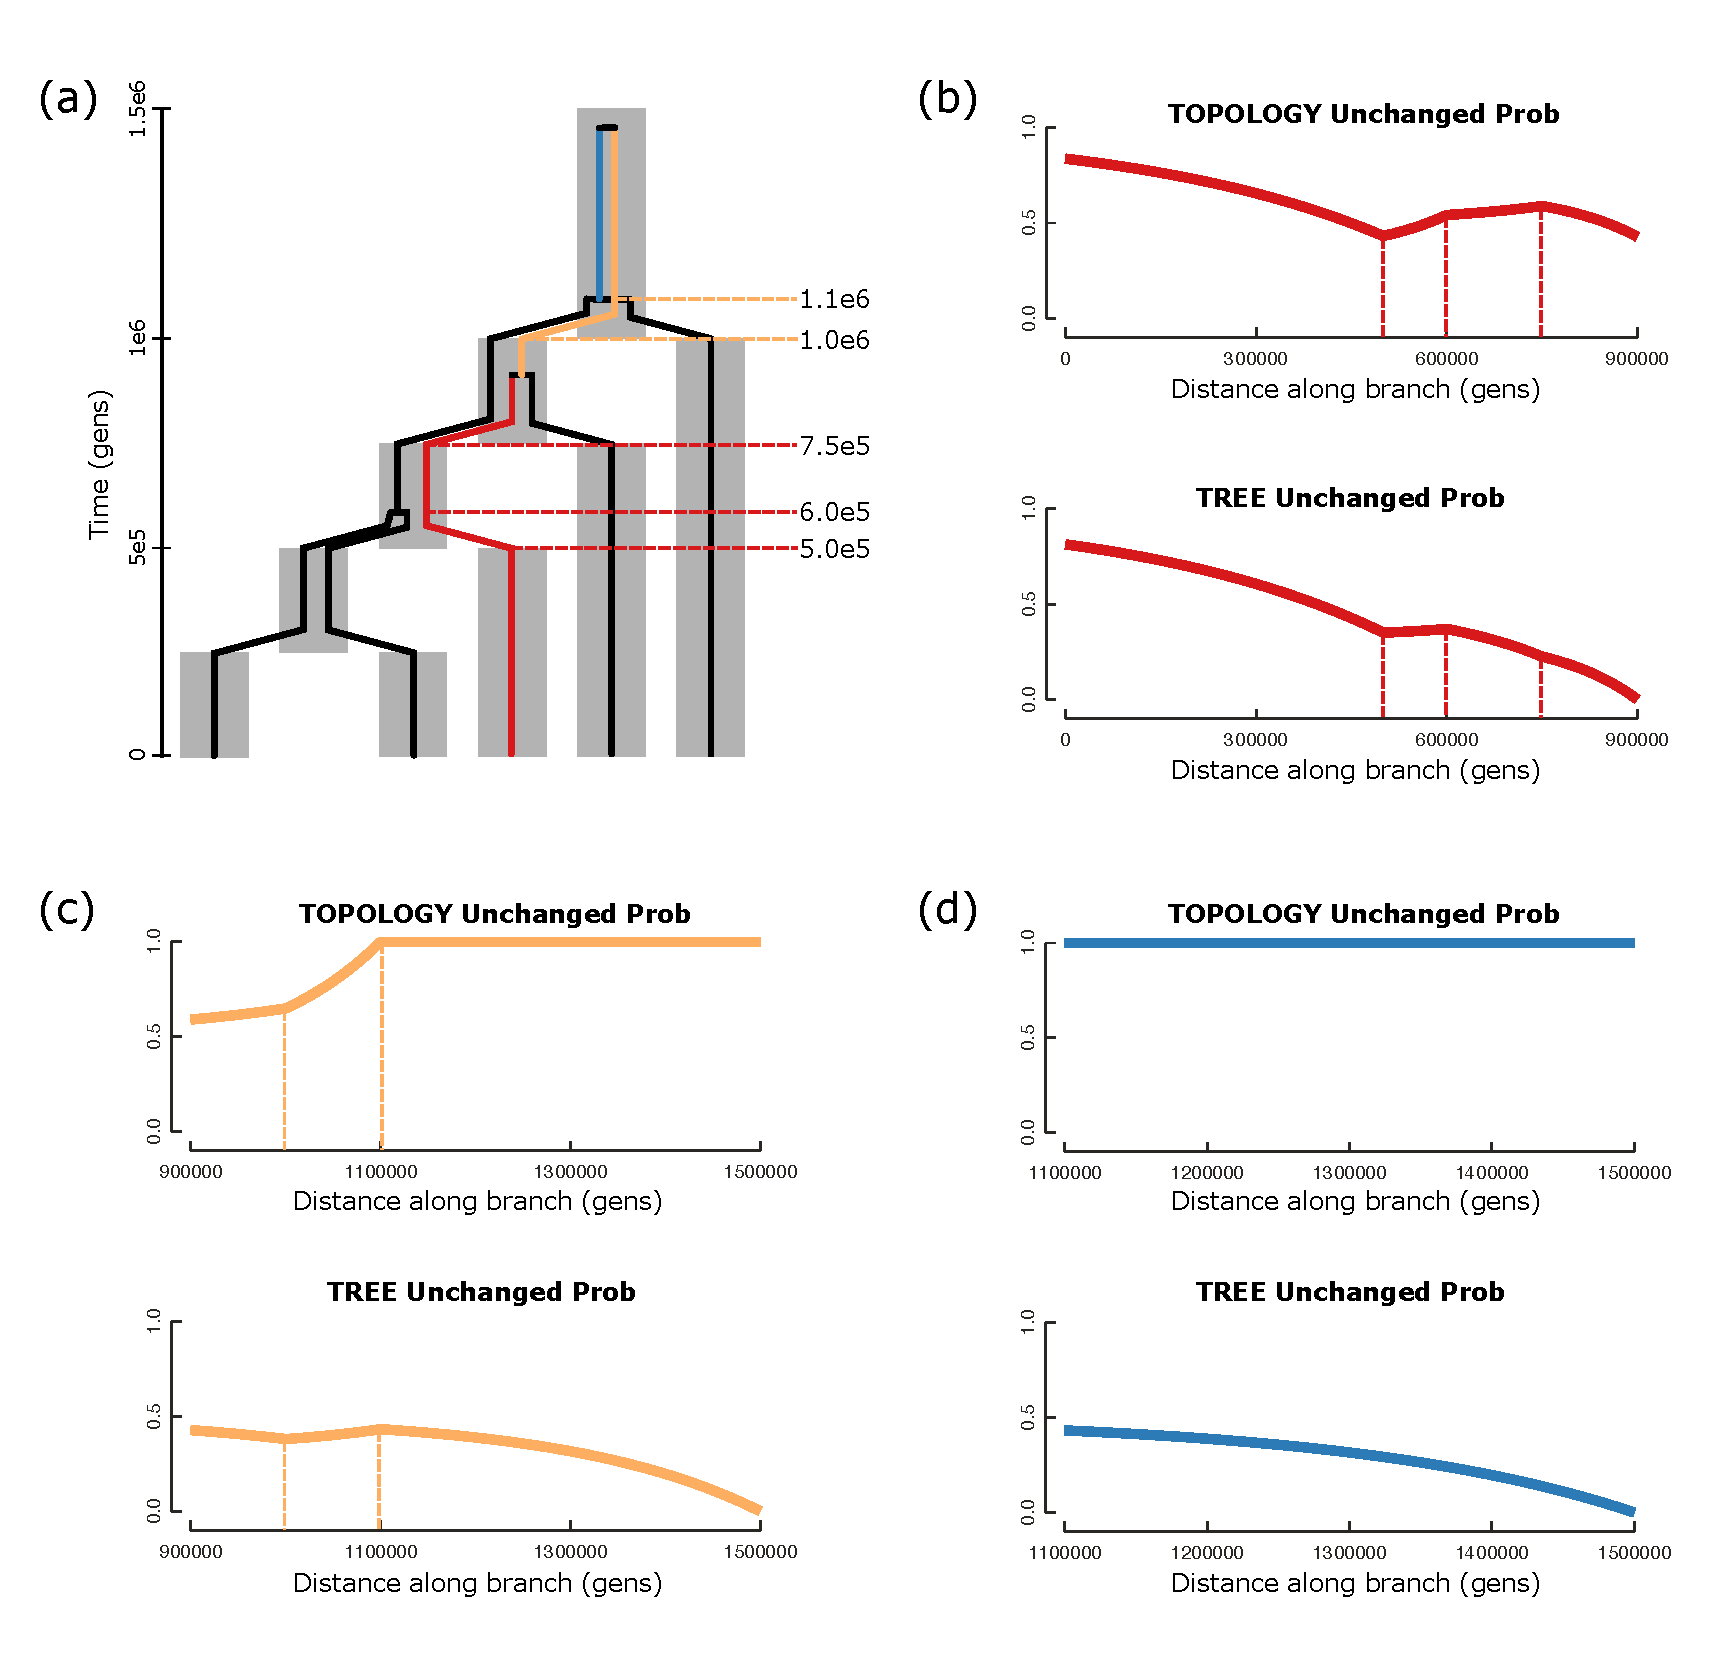
\includegraphics[width=0.9\textwidth]{figures/Fig4-bt_prob.pdf}
%	\caption{Probability that the topology and the tree remain unchanged, given a recombination event at a specific time on a specific branch. The species tree (a) was arbitrarily parameterized as being unbalanced with 5 tips, having internode distances of 2.5e5, and having constant Ne of 2e5. The embedded genealogical tree was randomly generated by \emph{ipcoal} using MSC probabilities. We selected three branches, indicated by three different colors, across which we calculated the probability that the topology would remain unchanged and the tree would remain unchanged if a recombination event were to occur at each time point on the branch (b-d). Dashed lines indicate the beginning and ending times of different intervals on each branch -- that is, either a relevant species tree divergence event or genealogy coalescence event.}
%	 \label{fig:fig3}
%\end{figure}

% This was tested for demographic models with different numbers of lineages;
% different numbers of samples among lineages; 
% and with different MSC model parameters, with the goal of representing scenarios
% spanning from population genetic to deeper-scale phylogenetic datasets. All
% datasets show nearly perfect matching between expected and simulated waiting 
% distances (Fig.~\ref{fig:fig-validation}). 

\subsection{Validation}


\begin{figure}[t]
	\centering
	%\fbox{\rule[-.5cm]{4cm}{4cm} \rule[-.5cm]{4cm}{0cm}}
	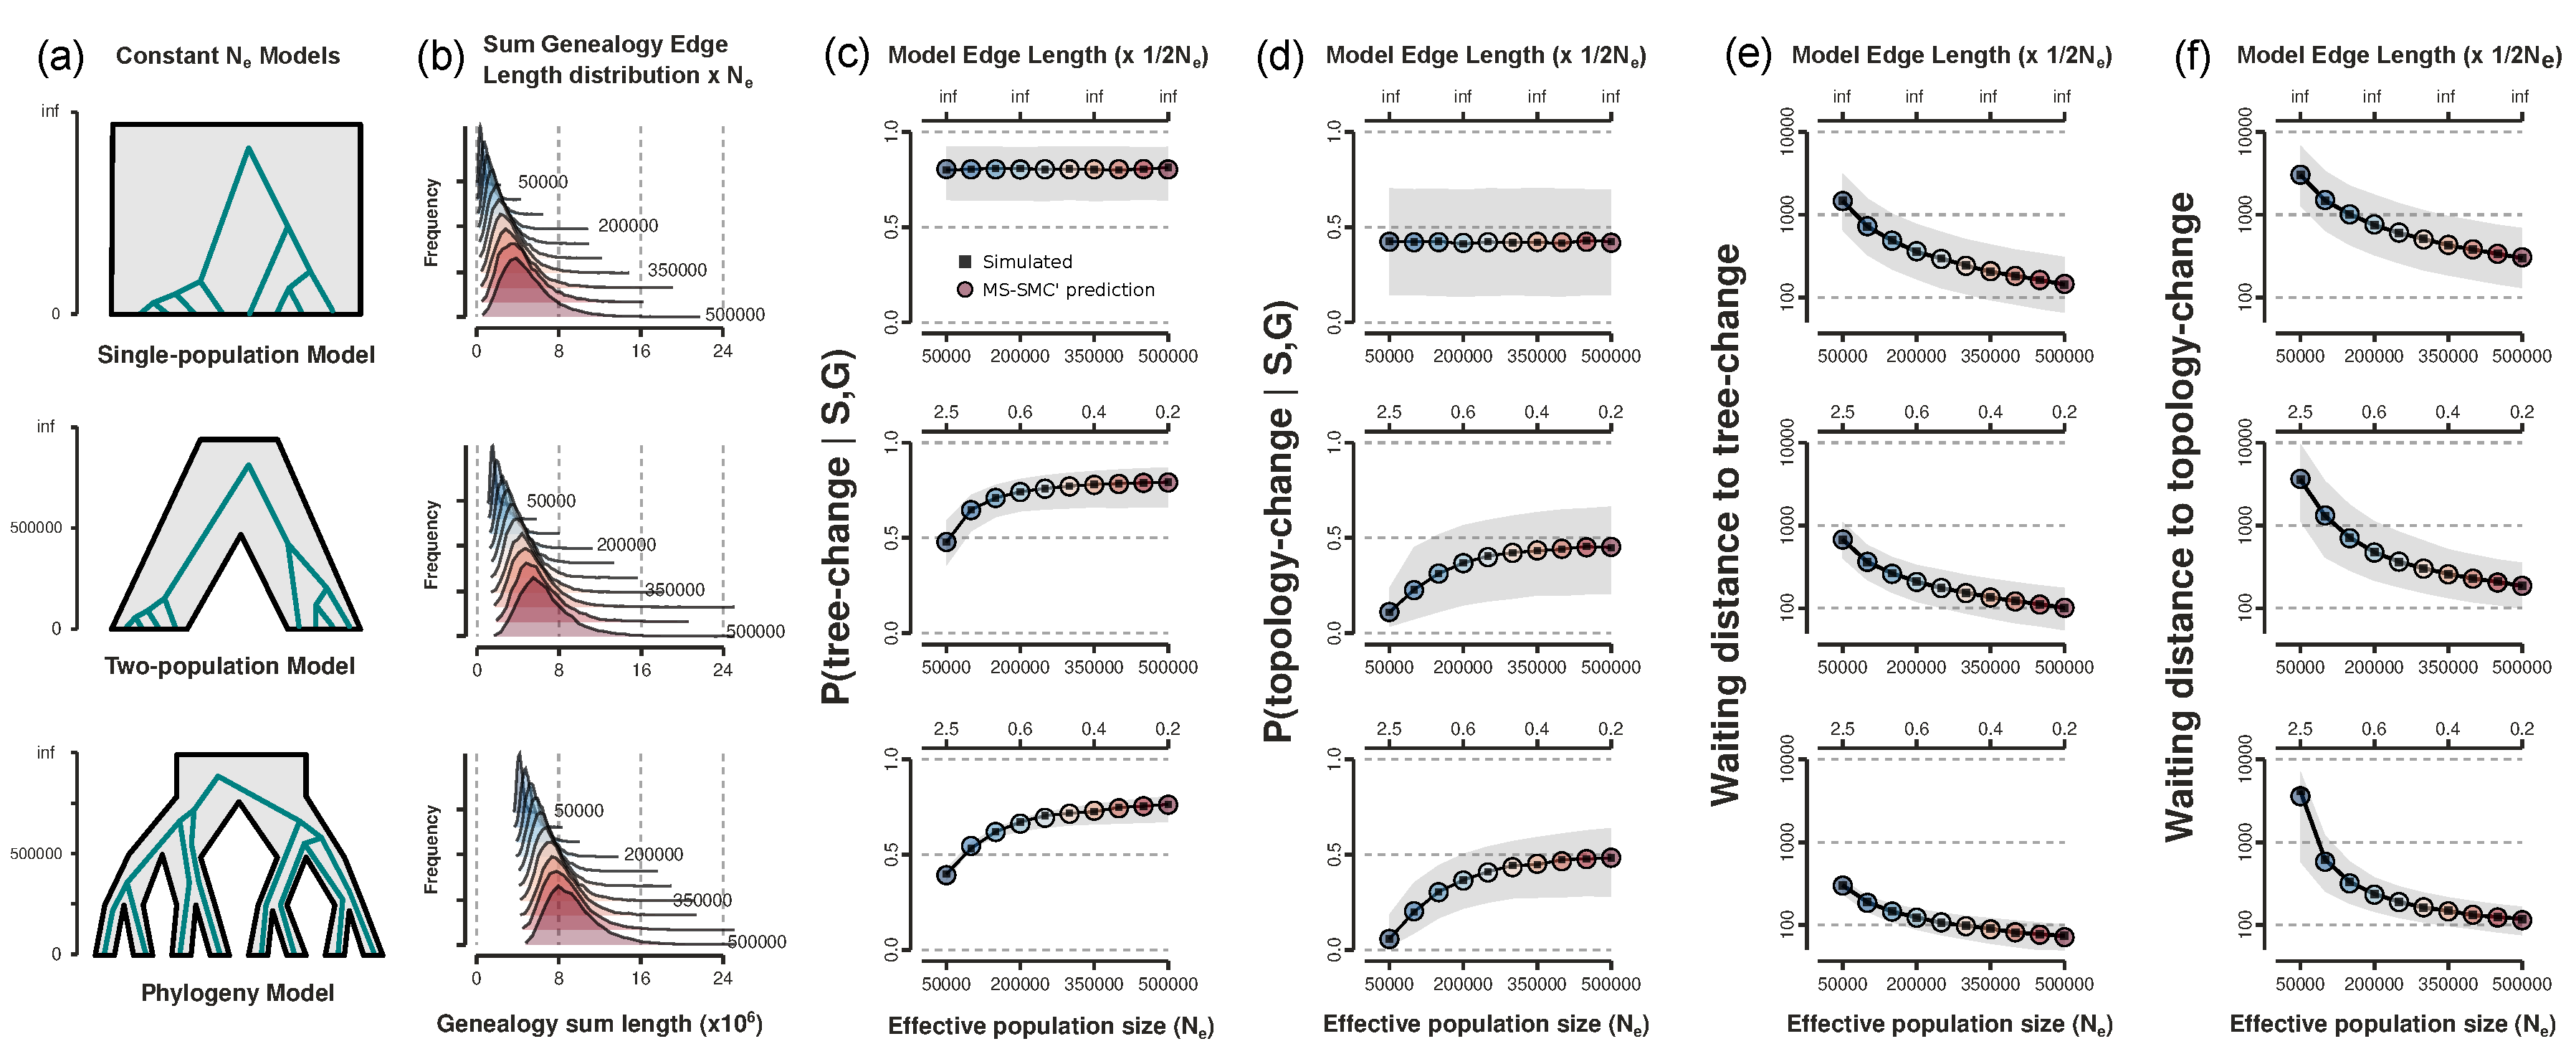
\includegraphics[width=0.99\textwidth]{figures/Fig4-final-validation4.pdf}
	\caption{
		MS-SMC' predictions validated against coalescent simulations.
		(a) Results are shown for three models containing 1, 2, or 8 
		populations. % among which genealogies for 8 samples were embedded. 
		For each model 10K tree sequences were simulated for 10 different
		constant $N_e$ values between 50K and 500K. 
		(b) The distributions of summed edge lengths of the first genealogy in 
		each tree sequence. 
		(c-d) The mean frequency (black square) at which the first observed 
		recombination event was a tree-change (c) or topology-change (d) in a 
		simulated tree sequence, and the mean (colored circle) and 95\% CI 
		(grey fill) of the predicted probability of tree or topology-change 
		calculated from the first embedded genealogy in each tree sequence. 
		Probabilities are constant with respect to $N_e$ in the single population
		%model, but vary in models with population structure
		model but vary in models with population structure
		%% ^removing all commas like this whenever I notice complex sentences beginning
		%% with an independent clause. (Or occassionally keeping the comma and just 
		%% adding a subject to the second clause.)
		(also shown with respect to species tree interval lengths in 
		coalescent units, across the top axis).
		% The probabilities of tree-change or topology-change are 
		% constant with respect to N$_e$ in a single population model, 
		% but vary in models with population structure (also shown with respect to 
		% species tree interval lengths in coalescent units, across the top axis). 
		(e-f) The mean waiting distance (black square) until the first observed 
		tree-change (e) or topology-change (f) in a simulated tree sequence, and the mean 
		(colored circle) and 95\% CI (grey fill) of predicted waiting distances calculated
		from the first embedded genealogy in each tree sequence.
		 % under the MS-SMC'. 
		% Predicted Predicted waiting distances Waiting distances between tree or topology-change events exhibit 
		% less variance for a given $N_e$ value in models with population structure. 
		% The MS-SMC' calculated waiting distance expectations match very closely to simulated values.
		% , however,
		% whereas the tree-change waiting distance is exact, the the topology-change waiting distance exhibits slight bias at very low 
		% N$_e$ values.
	}
	\label{fig:fig-validation}
\end{figure}

% we simulated data under 3 models to validate our results
To validate our analytical solutions for the probabilities of different 
recombination event outcomes and their associated waiting distances, 
we compared predictions of the MS-SMC' with results from stochastic 
coalescent simulations. 
We set up three scenarios with increasing amounts of population structure: 
a single-population model, a two-population model, and an 8-tip phylogeny model
(Fig.~\ref{fig:fig-validation}a). 
All analyses used a constant per-site per-generation recombination rate of 
2e-9 and simulated tree sequences using the coalescent with recombination 
(i.e., the "hudson" ancestry model in msprime as opposed to the "smc\_prime" model, 
which is an approximation), %unless specified, 
and the argument 
"record\_full\_arg=True" (to retain records of invisible recombination events). 
For each model we simulated genealogies for the same total number of samples
(8, unless specified), divided evenly among lineages when models 
include multiple populations (Fig.~\ref{fig:fig-validation}a). 
% When N$_e$ is low, 
% population structure is expected to have large effects, whereas when N$_e$ is 
% high, barriers imposed by population structure are expected to have 
% limited effects.

% results are composed of L, P, and L x P, which are calculated from sims in this way...
The exponential rate parameter ($\lambda$) for a probability distribution of waiting distances 
is a product of the per-site per-generation recombination rate ($r$), the sum 
of edge lengths on the current genealogy ($L(\mathcal{G})$), and the probability 
($\mathbb{P}$) of the specified event type (equations 9, 10, and 14). 
Across the three models examined, $r$ remains constant, but both $L(\mathcal{G})$ 
and $\mathbb{P}$ can vary due to population structure, where the effect of 
structure is scaled by $N_e$. 
Therefore, we examined $L(\mathcal{G})$, $\mathbb{P}$, and the expected waiting 
distance calculated from their product, for each demographic model across a range 
of $N_e$ values (Fig.~\ref{fig:fig-validation}b-f). 
For each value of $N_e$, 10K tree sequences were simulated that included at least 
one topology-change event. The empirical probabilities of tree-change and 
topology-change events were then simply measured %from simulated tree sequences 
as the mean observed frequency at which the first recombination event in each 
tree sequence was a tree or topology change. Similarly, empirical waiting 
distances were measured as the mean distance until the first observation of 
each event type. These simulated expectations were then compared with analytical
expectations computed under the MS-SMC', where probabilities and waiting distances 
were based only on the embedding of the first genealogy from each tree sequence 
into an MSC model parameterized to the specific constant $N_e$ value. 

% Given each starting genealogy,
% the probability of each event type, and the expected waiting distance to that event
% type, were calculated under the MS-SMC'. To compare this with the result of a 
% simulated coalescent with recombination process, we recorded the waiting distance 
% until each recombination event type first occurred in each tree sequence, and 
% also the frequency at which each event type occurred as the first event in a 
% tree sequence, as a measurement of its empirical probability.

% L and P have opposing effects on waiting distances given Ne
Population structure enforces a lower limit on the length of coalescent 
times by requiring that genealogies can be embedded in a species tree.
% This has an effect on $L(\mathcal{G})$ %at both low and high N$_e$
% of shifting both its minimum and mean 
This has the effect of shifting both the minimum and mean of 
$L(\mathcal{G})$ higher (Fig.~\ref{fig:fig-validation}b). 
Because the per-generation recombination rate interacts with
$L(\mathcal{G})$ (the opportunity over which recombination can occur) to
determine the frequency of recombination, larger $L(\mathcal{G})$ induced
by population structure will tend to decrease waiting distances between 
recombination events, all else being equal. 
However, all else does not remain equal. 
Population structure has a simultaneous opposing effect on waiting distances by 
decreasing the probability of tree or topology changes 
($\mathbb{P}$; Fig.~\ref{fig:fig-validation}c-d), especially at low $N_e$ values where 
species tree constraints can make tree or topology changes unlikely
to occur. This is a stark difference between the MS-SMC' framework and a 
single population model: The probability of a tree or topology change 
accompanying a recombination event is strongly associated with $N_e$ in the former but is not affected 
at all in the latter. 
%% Capitalization after a colon? APA says yes, Chicago says no.
%% (but I do think a colon is more appropriate than a semicolon here)
Consequently, in MSC models the waiting distances 
between each event type (Fig.~\ref{fig:fig-validation}e-f) represent a balance 
of the positive and negative effects of population structure on 
$L(\mathcal{G})$ and $\mathbb{P}$, respectively.

% Analytical predictions are very accurate, even better given SMC' approximation.
Our analytical predictions under the MS-SMC' converge accurately on 
the mean results from stochastic coalescent simulations 
(Fig.~\ref{fig:fig-validation}c-f). 
% Examining the relationship between MSC model parameters and expected 
% waiting distances also reveals ...
Moreover, by examining the variance in these predictions with 
respect to MSC model parameters we further gain insights into 
the information contained in spatial genealogical patterns.
% In a single population, the probability of a tree or topology change event
% is not only invariant with respect
For example, in the single population model there is high variance 
in both the probabilities of tree and topology changes, as well as in genealogy
lengths, at any given $N_e$ value. Consequently, waiting distances also 
exhibit high variance. Although waiting distances correlate with population $N_e$ 
in this model, the differences in mean waiting distances are small relative to the variance. 
By contrast, multispecies models exhibit much less variance in predicted probabilities 
of tree or topology changes given a set of MSC model parameters 
(Fig.~\ref{fig:fig-validation}c-d) and also exhibit less variation in genealogy
lengths. This leads to a stronger relationship between MSC model parameters and 
expected waiting distances (Fig.~\ref{fig:fig-validation}e-f), such that models
with different parameters have less overlap in waiting distance expectations.
Overall, this suggests that tree- and topology-change distances may contain more 
information in MSC models than in single population models.
% ; information that
% can be used for inferring demographic model parameters from waiting distances 
% in ARGs, or for inferring ARGs in the context of demography.

% The probabilities of tree or topology change events are highly variable in 
% the single population model, and constant with respect to $N_e$, whereas these probabilities exhibit 
% little variation for any given constant $N_e$-valued MSC model
% (Fig.~\ref{fig:fig-validation}c-d). This makes sense, considering 
% that genealogies in the latter models are constrained, especially
% when $N_e$ is low. This similarly leads to less variation in 
% expected waiting distances between tree or topology changes in 
% MSC models (Fig.~\ref{fig:fig-validation}e-f).
% where 
% genealogies are not constrained by population structure, and 
% thus exhibit no relationship with $N_e$. 
% By contrast, multispecies models exhibit much less variation
% in the probabilities of tree or topology change events given the 
% MSC model parameters (Fig.~\ref{fig:fig-validation}c-d). This makes
% sense, since the MSC model will constrain the types of genealogies
% that can be observed.
% Waiting distances to tree or topology-change events exhibit much less 
% variance for a given in MSC models than in the 
% The variance in waiting distance expectations at any examined $N_e$ value 
% are narrower in models with greater population structure, such as the 
% 8-population phylogeny model, than for the less structured models.
% Similarly, the magnitude of differences are also greater between waiting 
% distances given different N$_e$ in more highly structured MSC models.
% This suggests that tree and topology-change information is more informative 
% about demographic parameters (and vice versa) when population structure 
% is present. 
% We examine this further below to explore a likelihood framework 
% for MSC inference based on waiting distance expectations.

% As expected, 
% solutions for the probabilities of each event type (Fig.~\ref{fig:fig-validation}c-d), 
% and for waiting distances to tree-change events (Fig.~\ref{fig:fig-validation}e),
% appear as exact solutions, whereas the expected waiting distance to a topology-change
% event shows some bias at the lowest $N_e$ values (Fig.~\ref{fig:fig-validation}f). 

% waiting distances until tree or topology-change events decrease as
% values of N$_e$ increase, and topology-change waiting distances are always larger
% than tree-change waiting distances. 

\subsection{Bias in waiting distance estimation}
Estimated waiting distances under the MS-SMC’ harbor two potential sources of bias, 
the first stemming from assumptions of the SMC’ approximation, and the second from 
the approximate nature of waiting distance estimation for topology-change events. 
We examined both of these sources of error through comparison to stochastic simulations
and found that their effects are generally small, and that multispecies models exhibit 
a similar magnitude of error as single population coalescent models 
(Supplementary Materials; Fig.~\ref{fig:figS-bias-smc}, Fig.~\ref{fig:figS-bias-topo}).
The SMC' approximation contributes the greatest error in all models, leading to 
a slight under-estimation of waiting distances. This is most observable when variance
in waiting distances is high, as with topology-change waiting distances in models 
with low $N_e$. Future work could seek to find a correction for this bias.


\subsection{MS-SMC' likelihood inference framework}

\begin{figure}[t]
	\centering
	%\fbox{\rule[-.5cm]{4cm}{4cm} \rule[-.5cm]{4cm}{0cm}}
	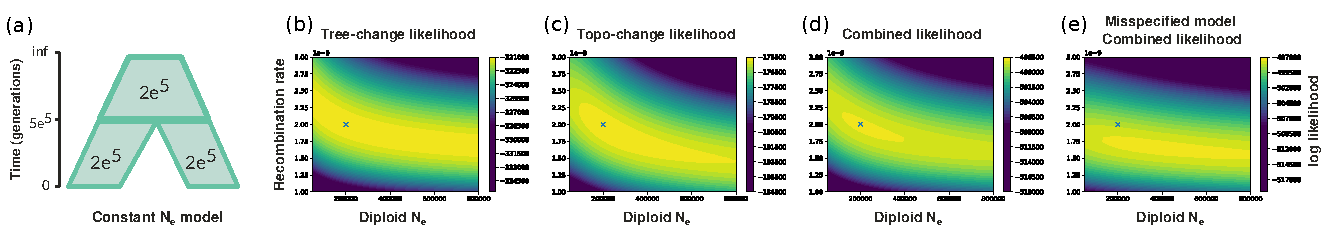
\includegraphics[width=0.99\textwidth]{figures/likelihood-figure3.pdf}
	\caption{
		MS-SMC' likelihood framework. (a) ARGs were simulated under a
		two-population species tree model with a constant $N_e$=200K and 
		$r$=2e$^{-9}$. (b) A joint log-likelihood surface for $N_e$ and 
		$r$ inferred from the distances between tree-change events, 
		(c) topology-change events; or (d) both. The true parameters are
		marked by an X. (e) If the MSC model is
		misspecified as a single-population model, but the data derive from 
		a two-population model, likelihood inference	is highly biased.
		% ARGs were 
		% simulated under a two-population species tree model with variable 
		% $N_e$. (e) A joint posterior distribution of $N_e$ parameters inferred 
		% by Bayesian MCMC from tree and topology-change waiting distances.
	}
	\label{fig:fig-likelihood}
\end{figure}

Based on the expectation that waiting distances are informative about 
MSC model parameters, we developed a maximum likelihood framework for inferring 
MSC model parameters from observed waiting distances between tree and/or topology 
change events. Here, we apply this method using the true distances between 
events in simulated ARGs. However, it could similarly be applied to inferred 
distances between events in an ARG proposed from sequence data. 

Given one or more ARGs, each composing a sequence of genealogies 
G = ($\mathcal{G}_1, \mathcal{G}_2, ..., \mathcal{G}_n$) and 
their interval lengths in the genome X = ($x_1, x_2, ..., x_n$), a subset 
of genealogies can be extracted representing unique genealogies between 
tree-change events, $G_g$ = ($\mathcal{G}_1, \mathcal{G}_i, ...$). The lengths 
between these events can be summed to get tree-change waiting distances
X$_g$ = ($\sum_{i=1}^j x_i, \sum_{i=j}^{k} x_i, ..., $). The same can be 
done for topology-change events. Then, given a parameterized species 
tree $\mathcal{S}$ and recombination rate $r$ we can infer a sequence of 
exponential rate parameters $\Lambda_g = (\lambda_1, \lambda_i, ...)$ for
each genealogy by using equations 10 or 14. 
The likelihood of each observed waiting distance (X$_g$) between tree or
topology change events can then be calculated from a series of exponential 
probability density functions (equation 8) parameterized by their 
corresponding rate parameters ($\Lambda_g$). 
The set of MSC model parameters -- which affect $\Lambda_g$ -- 
that maximize the summed log-likelihood of all observed distances 
between recombination events represents the maximum likelihood solution.

We first implemented this approach for a simple two-population model with 
constant $N_e$=200K and a population divergence at 500K generations. 
We simulated 100 independent ARGs, each 100Kb in length, using $r$=2e$^{-9}$, 
and we sampled four haplotypes per population. This 
yielded 51,487 tree-change events, with mean length 194bp, and 25,446 
topology-change events, with mean length 393bp. To examine the likelihood
surface we calculated the log-likelihood of joint parameters for $N_e$ and $r$, 
while keeping a fixed divergence time parameter, using a grid search across 41 evenly-spaced
values from $r=1e^{-9}$ to 3e$^{-9}$ and from $N_e$=50K to 800K. The likelihood
surface for tree-change distances exhibited a ridge containing the true 
parameter values (Fig.~\ref{fig:fig-likelihood}b), while the topology-change 
likelihood surface exhibited a distinct peak at the true values
(Fig.~\ref{fig:fig-likelihood}c). The summed log-likelihoods from both tree 
and topology change distances provided the most informative likelihood surface
(Fig.~\ref{fig:fig-likelihood}d).
We also inferred a likelihood surface for a misspecified model, in which 
the genealogies were generated under a 2-population model, but 
the $\Lambda_g$ rate parameters were calculated for a single population 
model with constant $N_e$. This model misspecification introduced a significant 
bias in parameter estimation, shifting the likelihood surface towards lower $r$ 
and higher $N_e$ (Fig.~\ref{fig:fig-likelihood}e). This demonstrates that even 
for a simple two population model, ignoring population structure can significantly
bias spatial genealogical inference methods.

\begin{figure}[t]
	\centering
	%\fbox{\rule[-.5cm]{4cm}{4cm} \rule[-.5cm]{4cm}{0cm}}
	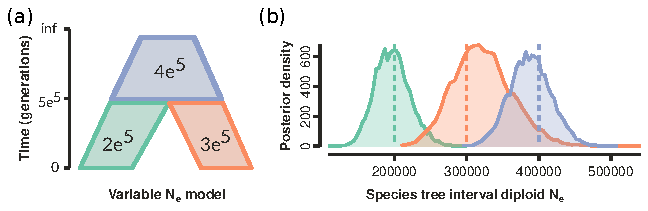
\includegraphics[width=0.55\textwidth]{figures/likelihood-posteriors.pdf}
	\caption{
		Joint inference of MSC model parameters using waiting distances 
		calculated under the MS-SMC'. (a) ARGs were simulated under a two-population 
		MSC model with variable $N_e$. (b) Posterior distributions of the three 
		$N_e$ parameters jointly inferred from tree- and topology-change waiting 
		distances.
	}
	\label{fig:fig-likelihood-posterior}
\end{figure}

To examine the accuracy of MSC parameter inference on more complex 
models, we implemented a Metropolis-Hastings Markov chain Monte Carlo 
(MCMC) algorithm to infer Bayesian posterior distributions of MSC model 
parameters under a 2-population model with variable $N_e$ 
(Fig.~\ref{fig:fig-likelihood-posterior}a).
The input ARGs were simulated using the same settings as above, 
%but under this more complex MSC model, and in this case, 
%we sampled 8 haplotypes per population. We set a uniform prior on 
except that we used this more complex MSC model and
sampled 8 haplotypes per population. We set a uniform prior on 
$N_e$ between 1e$^2$-1e$^7$ and ran the MCMC chain to sample 
10K values, sampling every 5th iteration after a 1K iteration 
burnin. For simplicity, we fixed the population divergence time to 
the correct value of 500K and focused solely on $N_e$ estimation. 

The resulting maximum \emph{a posteriori} probability estimates of 
model parameters are highly accurate, all falling within 0.5 
standard deviations of the true values 
(Fig.~\ref{fig:fig-likelihood-posterior}b). 
This result is encouraging, considering that it may be possible under
some MSC models for many different parameter combinations to yield 
similar waiting distance expectations, potentially causing identifiability
%issues. However, by combining information from both tree and topology 
%waiting distances this problem may be reduced. Our results suggest 
issues. However, combining information from both tree and topology 
waiting distances may help address this problem. Our results suggest 
that MSC model parameters will sometimes be identifiable from genealogical 
waiting distances, at least for relatively simple models like the ones
examined here. Further theoretical and empirical work will be needed
to explore this question in greater detail.
% Anecdotally, we found that using multiple independent ARGs improves 
% the accuracy of this joint inference method compared to a single 
% larger ARG. This suggests that ...


% MSC model parameters can predict waiting distances, we can also perform the 
% inverse operation, and find the maximum likelihood MSC model to explain a
% set of observed 

% Given a proposed or observed ARG, can we use MSC model parameters to find 
% ...

% Finally, we demonstrated that a known sequence of genealogies paired 
% with the accompanying observed waiting distances to next topological change 
% for each can be used to estimate the Ne value for species trees with different
% topologies (Fig.~\ref{fig:fig4}). We used two different species trees: one 
% imbalanced, 5-tip tree with internode branches of equal length, and one 10-tip tree
% with an irregular topology and branches of variable lengths. Both species 
% trees were assigned equal root heights of 1e6 generations and equal Ne values of 150000 on all 
% branches, and we simulated a 5e6-bp chromosome for each using \emph{ipcoal}. We broke each 
% chromosome down into its component "initial genealogies" -- those that start each segment 
% bounded by changes in topology -- and the accompanying segment lengths (i.e. waiting 
% distances). Using these values and a known recombination rate of 1e-9 recombs/bp/generation, 
% we calculated the likelihood that each of 41 proposed Ne values produced the set of 
% genealogies and waiting distances. Using this approach, we recovered a correctly inferred Ne 
% value of 150000 for both trees.


% with larger Ne values. This occurs for two reasons: first, genealogies with longer 
% branches have a higher probability of any recombination event occurring, since the
% rate is proportional to the sum of edge lengths; second, when Ne is large it is 
% more likely that many genealogy edges will exist in the same species tree intervals
% together, 
% coalescent events are more likely to occur deeper in time


% brief methods description
% Next, we tested the effect of variation in basic species tree parameters on expected waiting 
% distances to tree changes and topology changes (Fig.~\ref{fig:fig3}). We started with four 
% different species trees: two imbalanced and two balanced. For each pair, we used a large tree 
% (10 tips), and a small tree (5 tips) that was pruned from the large tree, with internode 
% distances kept the same. On each species tree, we generated 1000 random \emph{unlinked} 
% genealogies using MSC probabilities and using 
% each of 9 evenly spaced Ne values, ranging from 50000 to 250000. We calculated the expected 
% waiting distance 
% to a tree change and to a topology change for each genealogy/species tree pair, assuming a 
% recombination rate of 1e-9 recombs/bp/generation. In Fig.~\ref{fig:fig3}, we show the mean 
% expected waiting distances to tree and topology changes for each species tree and for each Ne 
% value. The decline in expected waiting distances across Ne values and from small to large 
% trees demonstrates that, on average, waiting distances to tree and topology changes decrease 
% with increasing numbers of tips sampled and with increasing Ne values. 





% \begin{figure}[t]
% 	\centering
% 	%\fbox{\rule[-.5cm]{4cm}{4cm} \rule[-.5cm]{4cm}{0cm}}
% 	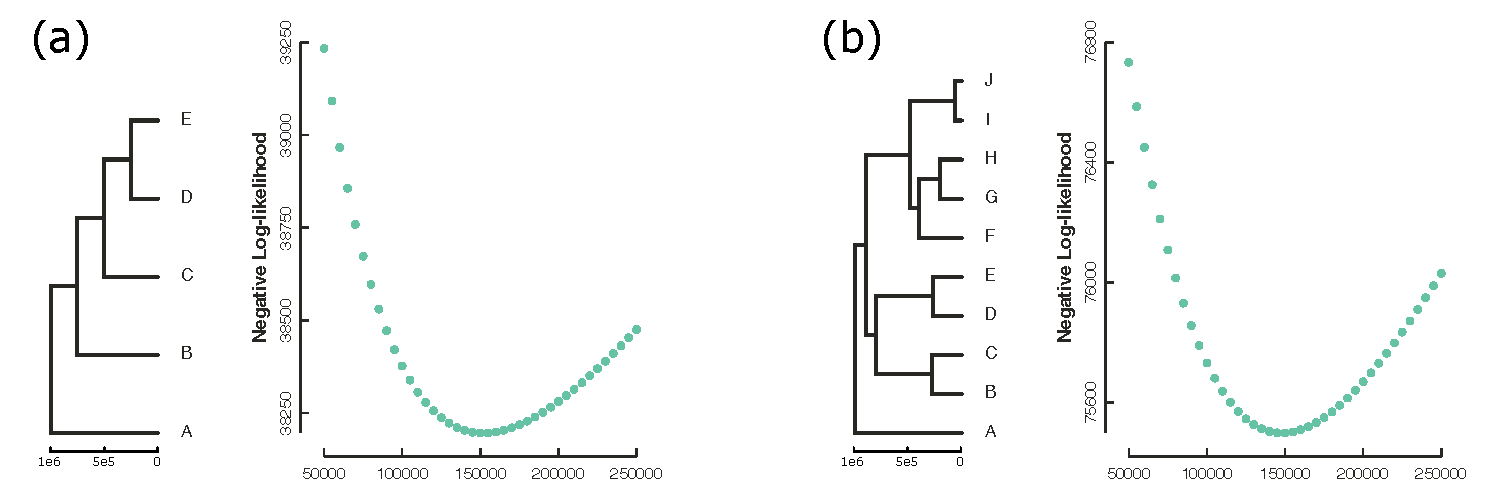
\includegraphics[width=0.9\textwidth]{figures/Fig6-constant_ne_inf.pdf}
% 	\caption{
% 		Inference of species tree Ne values from genealogies, observed waiting 
% 		distances to topology changes, and recombination rate. We generated two different 
% 		species trees: Both have root heights of 1e6 generations, but one has five tips, 
% 		an unbalanced topology, and identical internode lengths, while the other has ten 
% 		tips, an irregular topology, and irregular branch lengths. Using a recombination 
% 		rate of 1e-9 recombs/bp/generation and a constant Ne value of 150000 over all 
% 		branches, we generated a 5MB tree sequence from each species tree using 
% 		\emph{ipcoal}. Then, we decomposed the alignment into segments bounded by 
% 		topology changes in the genealogies, and we recorded the initial genealogy 
% 		for each segment. Finally, we calculated the likelihood of the set of 
% 		genealogies and waiting distances, along with the recombination rate, at 41 
% 		different proposed Ne values. For both sequence alignments, 150000 was 
% 		correctly inferred as the Ne value.
% 	}
% 	\label{fig:fig5}
% \end{figure}



%%%%%%%%%%%%%%%%%%%%%%%%%%%%%%%%%%%%%%%%%%%%%%%%%%%%%%%%%%%%%%%%%%%%%%%%%%%
%%%%%%%%%%%%%%%%%%%%%%%%%%%%%%%%%%%%%%%%%%%%%%%%%%%%%%%%%%%%%%%%%%%%%%%%%%%
%%%%%%%%%%%%%%%%%%%%%%%%%%%%%%%%%%%%%%%%%%%%%%%%%%%%%%%%%%%%%%%%%%%%%%%%%%%
%%%%%%%%%%%%%%%%%%%%%%%%%%%%%%%%%%%%%%%%%%%%%%%%%%%%%%%%%%%%%%%%%%%%%%%%%%%
%%%%%%%%%%%%%%%%%%%%%%%%%%%%%%%%%%%%%%%%%%%%%%%%%%%%%%%%%%%%%%%%%%%%%%%%%%%
%%%%%%%%%%%%%%%%%%%%%%%%%%%%%%%%%%%%%%%%%%%%%%%%%%%%%%%%%%%%%%%%%%%%%%%%%%%
%%%%%%%%%%%%%%%%%%%%%%%%%%%%%%%%%%%%%%%%%%%%%%%%%%%%%%%%%%%%%%%%%%%%%%%%%%%
%%%%%%%%%%%%%%%%%%%%%%%%%%%%%%%%%%%%%%%%%%%%%%%%%%%%%%%%%%%%%%%%%%%%%%%%%%%
%%%%%%%%%%%%%%%%%%%%%%%%%%%%%%%%%%%%%%%%%%%%%%%%%%%%%%%%%%%%%%%%%%%%%%%%%%%
%%%%%%%%%%%%%%%%%%%%%%%%%%%%%%%%%%%%%%%%%%%%%%%%%%%%%%%%%%%%%%%%%%%%%%%%%%%
%%%%%%%%%%%%%%%%%%%%%%%%%%%%%%%%%%%%%%%%%%%%%%%%%%%%%%%%%%%%%%%%%%%%%%%%%%%
%%%%%%%%%%%%%%%%%%%%%%%%%%%%%%%%%%%%%%%%%%%%%%%%%%%%%%%%%%%%%%%%%%%%%%%%%%%
%%%%%%%%%%%%%%%%%%%%%%%%%%%%%%%%%%%%%%%%%%%%%%%%%%%%%%%%%%%%%%%%%%%%%%%%%%%
%%%%%%%%%%%%%%%%%%%%%%%%%%%%%%%%%%%%%%%%%%%%%%%%%%%%%%%%%%%%%%%%%%%%%%%%%%%


\section{Discussion}



% Summarize what we did
%We began with a simple question: what is the expected turnover rate in 
%topologies along a genome under a species tree model? We generalized a 
%recent solution that used a single population and constant Ne \citep{deng_distribution_2021}, instead 
We solved for the expected turnover rate in genealogical trees and topologies 
along a genome under an arbitrary species tree topology with arbitrary 
divergence times, and with arbitrary Ne values for each species tree branch.
%structuring the equations to accept an arbitrary species tree topology 
%and a different, arbitrary Ne value for each species tree branch. 
These solutions, extended from initial work by \citep{deng_distribution_2021}, 
lay a groundwork for exploring how variation in species tree parameters 
affects neutral expectations of genealogical heterogeneity across chromosomes.

% what do our results mean overall.
A primary result of our work is solving the mechanistic link between a given species tree 
and the length of a genomic interval representing a single genealogy 
(i.e. calculating the expected waiting distance until a genealogy change). 
With our analytical results it is clear how MSC parameters of divergence times and 
effective population sizes influence these waiting distances, most obviously 
by constraining the number and identity of available lineages and by determining 
the coalescence rate in each branch of the species tree. 
These parameters also affect the rate of recombination events along the genome, since the 
number of recombination events per base pair is dependent on the total branch 
length of each underlying genealogy. By preventing coalescence between select lineages toward the present, 
species tree divergence events enforce minimum branch lengths for the genealogies, 
increasing the number of recombination events per base pair. Similarly, by affecting coalescence rates, variation in Ne 
affects the per-base-pair recombination rate. This is because coalescences farther back in time 
(which are expected to be more common if Ne is large)
increase the total branch lengths of the genealogies.
Topological and sampling parameters, including tree shape, tree size (i.e. number of tips), 
and the distribution of samples among species tree 
lineages, similarly affect the expected distances until genealogy 
changes. These factors all exert their influence via the same general mechanisms as above: they affect the 
probability of coalescence among certain lineages by constraining the availability of those lineages 
for coalescence with each other, and they influence the 
rate of recombination by affecting the total branch length of each genealogy. 
Taken together, it is clear that the scale at which we observe neutral turnover across 
genealogies is highly dependent on the species tree model. The potential 
intricacy of this species tree model alongside expected variation in individual genealogies 
can lead to patterns of genealogical turnover (and therefore, linkage) that are highly complex. 
%Because of low levels of incomplete lineage sorting, highly 
%structured models might have much longer waiting distances than single-population models. 
Previously, the expected linkage in phylogenetic datasets could only be computed 
through exhaustive simulations (e.g., \citep{mckenzie_multispecies_2020}. While such methods
are practical for estimating the \emph{mean} linkage across all genealogies under a 
specific demographic model, they are less helpful for estimating the 
persistence of \emph{individual} genealogies in localized regions. To generate an approximate distribution 
of waiting distances locally on a chromosome using simulation methods, 
simulations generating a full probability distribution must be 
run individually for each genealogy in the sequence. 
Although this is benign across single, short segments, it is not a tractable solution across long 
sequences of genealogies and/or across many replicates. 

% importance to phylogenetics
%By accounting for the genomic heterogeneity that is expected due to incomplete 
%lineage sorting, t
While the multispecies coalescent model has facilitated the widespread 
use of multilocus data for phylogenetic inference by accounting for genomic heterogeneity, 
it does not consider autocorrelation along the genome due to linkage.
%, and it assumes 
%that each locus represents only a single genealogy. In reality, these assumptions might 
%often be violated \citep{gatesy_concatenation_2013}. 
%As phylogenetic systematics 
%continues to turn toward whole genomes, methods should seek to extend the MSC to take advantage 
%of the increased resolution offered by genomic data. 
Specifically, the MSC overlooks the process of recombination, assuming that each locus 
represents a single genetic history and that multiple loci are completely unlinked from one another. 
From our results, and from previous work, we know that species tree parameters and recombination 
rates will dictate the rate and magnitude of genealogical turnover along a chromosome, 
potentially resulting in -- in some cases -- high linkage between loci, and 
-- in other cases -- multiple genealogical topologies 
per locus. Therefore, not accounting for recombination might mislead 
summary statistics methods \citep{liu2010maximum,gatesy_concatenation_2013,zhang2018astral}. 
Some methods bypass genealogy inference by operating directly on SNP 
frequencies \citep{bryant2012inferring,chifman2014quartet,vachaspati2018svdquest}, 
and therefore might largely avoid bias from ignoring recombination. 
To extend these SNP-based methods and/or to improve gene-tree-based methods to better delimit gene tree breakpoints, 
we propose that incorporating the rates of turnover observed in the data as 
information could actually offer useful new information for inferring the species tree 
model that generated it. 


%Inference of genealogies along a chromosome is a common goal in population genetics, and similar efforts have been undertaken in phylogenetics. Often, the goal of such efforts is to detect signals of introgression or selection. However, the phylogenetic approaches usually do not explicitly incorporate a model for recombination \citep[e.g.,][]{li2019recombination}. A notable exception to this is ARGweaver-D, which accepts models with population divergence and migration event parameters. Rather than derive probabilities of sequences of genealogical trees, ARGweaver-D uses an MCMC to sample the sequences. This approach is a powerful extension of the single-population ARGweaver method and has been applied successfully to study evolution of hominins, but it is limited to small numbers of samples. Challenges remain for studying properties of tree sequences for larger sets of samples.
%Rather than inferring the species tree model, many modern genomic methods aim to 
%These  methods aim to 
%infer ARGs analyzing local patterns along the genome.
The ultimate goal of ARG inference in phylogenomic or population genomic studies
is often to detect signals of introgression or selection. 
However, even in the case of a neutral coalescent process 
with constant effective population sizes and with a constant recombination rate 
across the genome, highly structured demographic models can exhibit
high variance in the expected waiting distances until genealogical 
topology changes (e.g. Fig.~\ref{fig:fig-validation}). As genealogical trees and 
topologies vary along the genome, the waiting distance probability distribution 
does too -- the result of this is that certain genealogies are expected to persist longer than others 
due to their topology and coalescence times relative to the demographic model. 
Until now, there has been no analytical approach for generating a null hypothesis 
that describes the expected length of a region spanned by a particular genealogy under absolute neutrality.
Our results allow us to calculate this null expectations and to probe null hypotheses concerning the probability 
of observing specific waiting distances under different demographic models. 
Of course, the MSC already allowed us to calculate the probability of observing a particular 
genealogy at some location in the genome, but the equations here represent a further step by 
generating a density function that represents the likelihood of \emph{persistence} 
of that topology across some region, under neutrality alone. 
This finding is particularly important for the practice of identifying evidence 
of selection or introgression based on the spatial distribution of gene tree 
patterns, which is an increasingly popular goal of phylogenomic studies. 
For example, sliding-window analyses for detecting introgression have 
been used to identify putatively introgressed loci in \emph{Heliconius} 
butterflies \citep{zhang2016genome} and felids \citep{li2019recombination}. 
Further, since we are able to calculate the likelihood of observing any sequence of waiting 
distances associated with an ARG, we speculate that incorporating our waiting distance 
expectations could be incorporated into ARG-inference methods like
ARGweaver, ARGweaver-D, tsinfer, and relate \citep{rasmussen2014genome, hubisz2020inference, kelleher2019inferring, speidel2019method} 
as an additional source of information. 

%Our results here highlight the fact that demographic history plays an 
%important role in establishing a null hypothesis for the expected rate 
%of turnover of genealogies along the genome.

%Beyond its use for detecting patterns resulting from 
%non-neutral processes, incorporating recombination in phylogenetic-scale models 
%could also help improve species tree inference. For example, to the extent that 
%they are observable, the empirical distribution of waiting distances to topology 
%changes might be inferred and compared against the expected waiting distances for 
%a proposed species tree model (e.g., \textbf{Figure 5}). Further approaches could 
%determine the distribution of waiting distances to specific types of topology 
%changes, such as those that split up a focal clade.


%Topological gravity wells. 
%Even in the case of a neutral coalescent process 
%with constant effective populations sizes and constant recombination rate 
%across the span of a genome, highly structured demographic models can exhibit
%high spatial variance in the expected waiting distances until topology changes. 
%This finding is particularly important for the practice of identifying evidence 
%of selection or introgression based on the spatial distribution of gene tree 
%patterns. For example, sliding-window analyses for detecting introgression have 
%been used to identify putatively introgressed loci in \emph{Heliconius} butterflies \citep{zhang2016genome}. 
%Our results here highlight the fact that the demographic history of this group is 
%important for establishing a null hypothesis for the expected rate of turnover of genealogies along the genome.

%Examples: Heliconius. 




\subsection{Acknowledgements}
This work was supported by the National Science Foundation 
(NSF DEB-2046813 awarded to D.A.R.E. and NSF Graduate Research Fellowship DGE 16-44869 awarded 
to P.F.M.). Thanks to Yun Deng for guidance on preliminary ideas and to the Eaton Lab for valuable feedback.


%\subsection{Citations}
%Citations use \verb+natbib+. The documentation may be found at
%\begin{center}
%	\url{http://mirrors.ctan.org/macros/latex/contrib/natbib/natnotes.pdf}
%\end{center}

%Here is an example usage of the two main commands (\verb+citet+ and \verb+citep+): Some people thought a thing \citep{kour2014real, hadash2018estimate} but other people thought something else \citep{kour2014fast}. Many people have speculated that if we knew exactly why \citet{kour2014fast} thought this\dots

%\subsection{Figures}
%\lipsum[10]
%See Figure \ref{fig:fig1}. Here is how you add footnotes. %\footnote{Sample of the first footnote.}
%\lipsum[11]

%\begin{figure}
%	\centering
	%\fbox{\rule[-.5cm]{4cm}{4cm} \rule[-.5cm]{4cm}{0cm}}
%	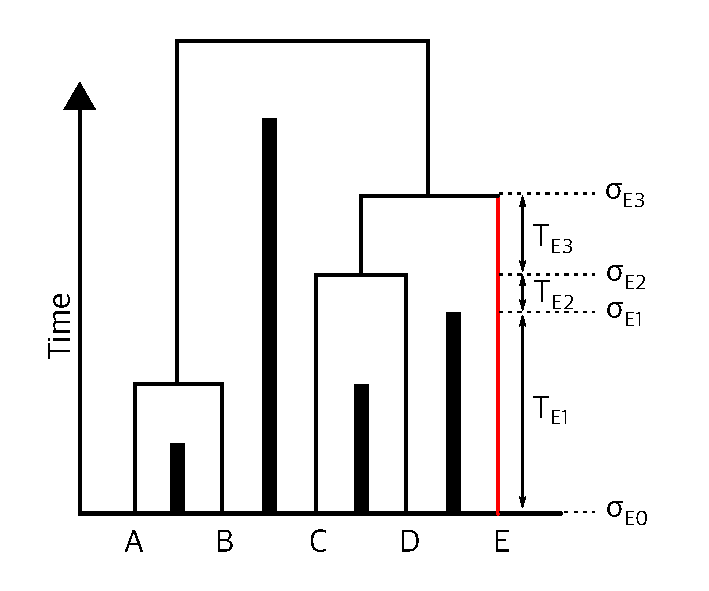
\includegraphics[width=0.6\textwidth]{genealogy_ebranch.pdf}
%	\caption{Sample figure caption.}
%	\label{fig:fig1}
%\end{figure}

%\subsection{Tables}
%See awesome Table~\ref{tab:table}.

%The documentation for \verb+booktabs+ (`Publication quality tables in LaTeX') is available from:
%\begin{center}
%	\url{https://www.ctan.org/pkg/booktabs}
%\end{center}


%\begin{table}
%	\caption{Sample table title}
%	\centering
%	\begin{tabular}{lll}
%		\toprule
%		\multicolumn{2}{c}{Part}                   \\
%		\cmidrule(r){1-2}
%		Name     & Description     & Size ($\mu$m) \\
%		\midrule
%		Dendrite & Input terminal  & $\sim$100     \\
%		Axon     & Output terminal & $\sim$10      \\
%		Soma     & Cell body       & up to $10^6$  \\
%		\bottomrule
%	\end{tabular}
%	\label{tab:table}
%\end{table}

%\subsection{Lists}
%\begin{itemize}
%	\item Lorem ipsum dolor sit amet
%	\item consectetur adipiscing elit.
%	\item Aliquam dignissim blandit est, in dictum tortor gravida eget. In ac rutrum magna.
%\end{itemize}


\bibliographystyle{ecol_let}
\bibliography{references}  

%%% Uncomment this line and comment out the ``thebibliography'' section below to use the external .bib file (using bibtex) .


%%% Uncomment this section and comment out the \bibliography{references} line above to use inline references.
% \begin{thebibliography}{1}

% 	\bibitem{kour2014real}
% 	George Kour and Raid Saabne.
% 	\newblock Real-time segmentation of on-line handwritten arabic script.
% 	\newblock In {\em Frontiers in Handwriting Recognition (ICFHR), 2014 14th
% 			International Conference on}, pages 417--422. IEEE, 2014.

% 	\bibitem{kour2014fast}
% 	George Kour and Raid Saabne.
% 	\newblock Fast classification of handwritten on-line arabic characters.
% 	\newblock In {\em Soft Computing and Pattern Recognition (SoCPaR), 2014 6th
% 			International Conference of}, pages 312--318. IEEE, 2014.

% 	\bibitem{hadash2018estimate}
% 	Guy Hadash, Einat Kermany, Boaz Carmeli, Ofer Lavi, George Kour, and Alon
% 	Jacovi.
% 	\newblock Estimate and replace: A novel approach to integrating deep neural
% 	networks with existing applications.
% 	\newblock {\em arXiv preprint arXiv:1804.09028}, 2018.

%\end{thebibliography}



%%%%%%%%%%%%%%%%%%%%%%%%%%%%%%%%%%%%%%%%%%%%%%%%%%%%%%%%%%%%%%%%%%%%%%%%%%%
%%%%%%%%%%%%%%%%%%%%%%%%%%%%%%%%%%%%%%%%%%%%%%%%%%%%%%%%%%%%%%%%%%%%%%%%%%%
%%%%%%%%%%%%%%%%%%%%%%%%%%%%%%%%%%%%%%%%%%%%%%%%%%%%%%%%%%%%%%%%%%%%%%%%%%%
%%%%%%%%%%%%%%%%%%%%%%%%%%%%%%%%%%%%%%%%%%%%%%%%%%%%%%%%%%%%%%%%%%%%%%%%%%%
%%%%%%%%%%%%%%%%%%%%%%%%%%%%%%%%%%%%%%%%%%%%%%%%%%%%%%%%%%%%%%%%%%%%%%%%%%%
%%%%%%%%%%%%%%%%%%%%%%%%%%%%%%%%%%%%%%%%%%%%%%%%%%%%%%%%%%%%%%%%%%%%%%%%%%%
%%%%%%%%%%%%%%%%%%%%%%%%%%%%%%%%%%%%%%%%%%%%%%%%%%%%%%%%%%%%%%%%%%%%%%%%%%%



\newpage

\beginsupplement
\section{Supplementary Information}

\subsection{Supplementary Figures}

\begin{figure}[p]
	\centering
	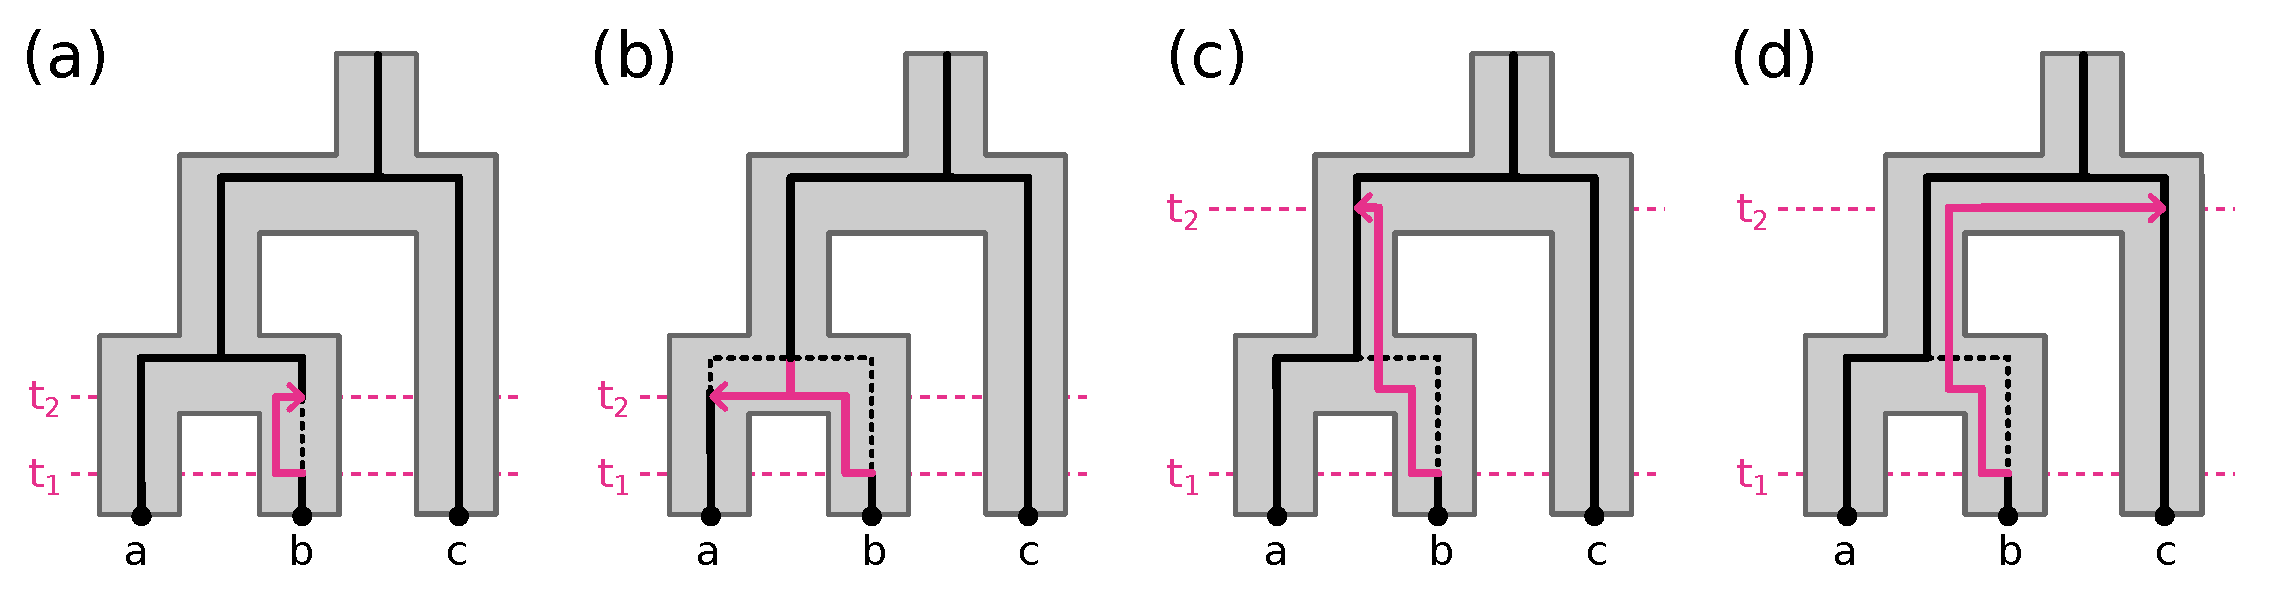
\includegraphics[width=0.9\textwidth]{figures/Fig2-new-recomb-types.pdf}
	\caption{
		Four categories of outcomes of a recombination event occurring on a
		genealogy at time t$_1$ and the detached subtree re-coalescing with
		the remaining lineages under the SMC' process at time t$_2$. (a) The
		detached subtree re-coalesces with the original lineage from which it
		was detached leading to no change between the starting genealogy and 
		subsequent genealogy. (b) The detached subtree re-coalesces with its
		sibling lineage prior to their previous coalescence, leading to a shortening
		of their coalescence time. (c) The detached subtree re-coalesces with
		its parent lineage, leading to a lengthening of the coalescent time 
		between the detached subtree lineage and its sibling lineage. (d) The
		detached subtree re-coalesces with a lineage other than itself, its sibling,
		or its parent lineage, leading to a topology-change. 
	}
     \label{fig:figS-recomb-types}
\end{figure}

% \begin{landscape}
	% 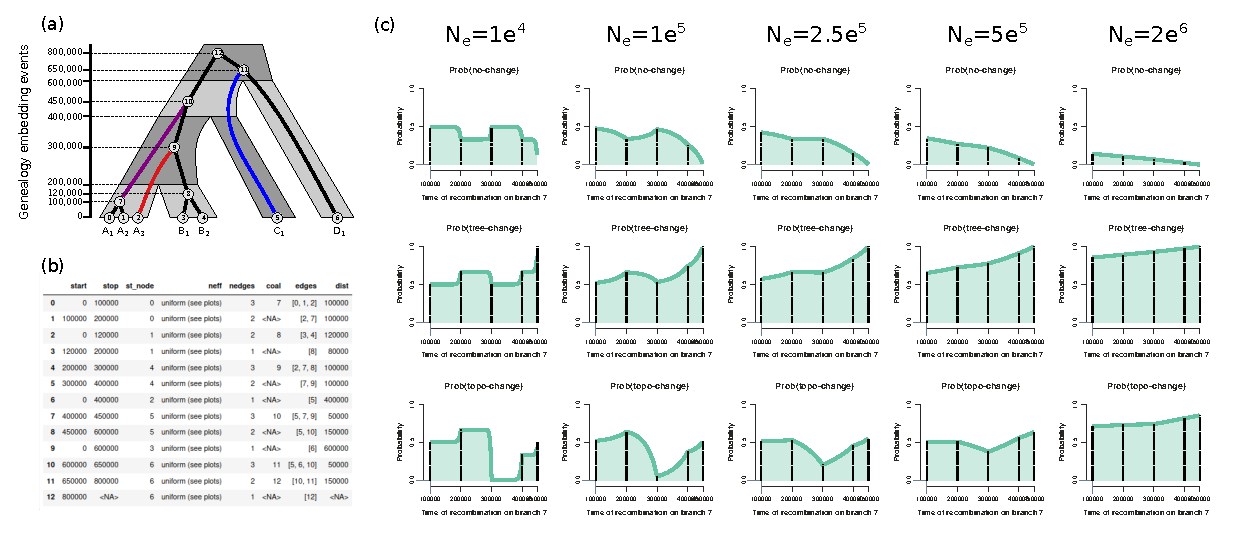
\includegraphics[width=0.99\linewidth,keepaspectratio]{figures/Fig-S2-edge-probabilities.pdf}
% \end{landscape}

\begin{figure}[p]
	\centering
	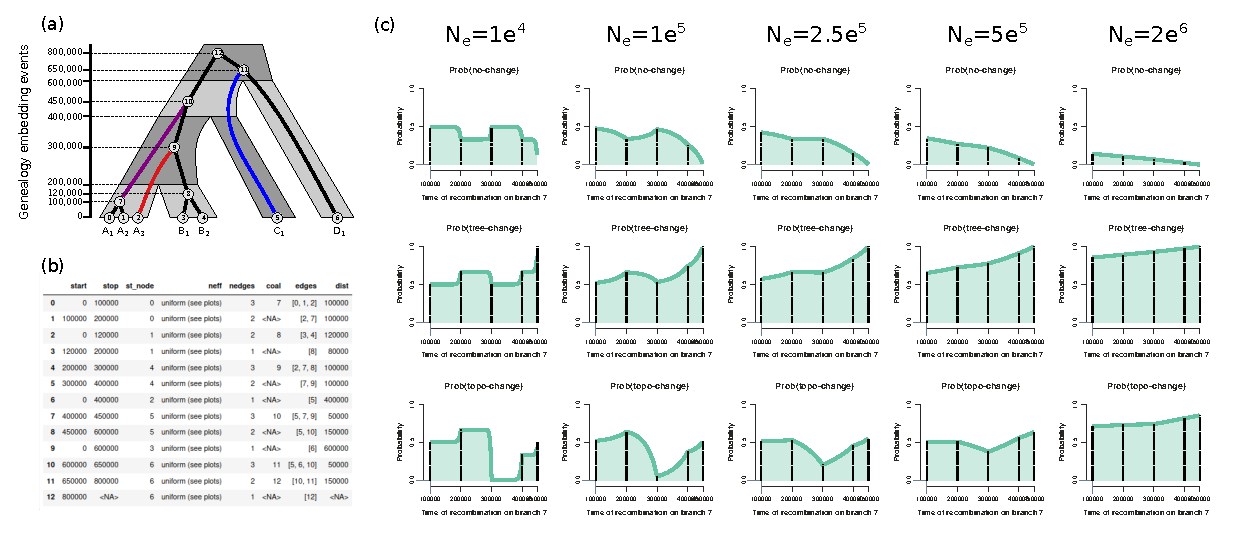
\includegraphics[width=0.99\textwidth]{figures/Fig-S2-edge-probabilities.pdf}	
	\caption{
		Probabilities of different recombination event outcomes for a selected 
		genealogy edge as a function of the time at which recombination occurs 
		and of the constant effective population size.
		(a) An MSC model with edge lengths in units of generations and an example
		genealogy embedded. (b) An example genealogy embedding table for the MSC
		model and genealogy. (c) Probabilities of different recombination event
		outcomes across genealogy edge 7. When $N_e$ is low, probabilities are 
		nearly constant within each interval since re-coalescence in later intervals
		is unlikely. When $N_e$ is high, probabilities change nearly monotonically 
		across the length of an edge since population structure does little
		to constrain the time of re-coalescence.
	}
     \label{fig:figS-edge-probabilities}
\end{figure}

\newpage


% \section{Appendix: Derivations}
% \subsection{Derivations of the Multispecies Sequentially Markov Coalescent (MS-SMC')}


% \subsection{testing}

% and also act in opposing directions, such that their
% combined effect is further reduced.

% The MS-SMC’ harbors two potential sources of bias. The first affects only 
% topology-change waiting distances, and appears to have a relatively small effect. 
% This stems from the potential for topology-change probabilities to vary spatially
% across a distance of the genome between two topology-change events as a result 
% of intermediate tree-change events 
% (e.g., the second and third recombination events in Fig.~\ref{fig:fig2}).
% Consequently, unlike the exact solution for tree-change waiting distances, 
% topology-change waiting distances represent an approximation. 
% Using  coalescent simulations we measured the variance in probabilities of 
% topology-change across the spanned intervals between topology-change 
% events (Supplemental Materials for methods and results; Fig.~\ref{fig:figS-bias-topo}).
% Multispecies models do not exhibit greater error than single population models.
% A second source of bias stems from assumptions of the SMC’ approximation to the full 
% coalescent with recombination model. By not modeling recombination events that 
% occurred among ancestors that do not contribute genetic material
% to the samples, SMC'-based methods tend to under-estimate recombination events. 
% The frequency of such events in single populations is small \citep{mcvean2005approximating}. 
% We performed coalescent simulations to examine how this error increases in multi-species models 
% (see Supplemental Materials for methods), and found that our MS-SMC' estimations exhibit 
% almost no error when compared to data simulated under the SMC' process, but approximately
% -5\% compared to the full coalescent with recombination model (Fig.~\ref{fig:figS-bias-smc}). 

% ....
% ...
% A second source of error affects only topology waiting distances. ...
% he SMC’ approximation to the coalescent with recombination is expected to deviate more signifi-
% cantly from the full model that it is approximating as the number of recombination events that the SMC’
% does not model (among ancestors that do not contribute genetic material to sampled descendants) increases.
% By not modeling some recombination events the SMC’ will tend to over-estimate waiting distances be-
% tween tree or topology change events.

% and the second from the approximate 
% nature of waiting distance estimation for topology-change events. We examined both 
% of these sources of error through comparison to stochastic simulations
% and found that their effects are generally negligible, and also act in opposing directions, such that their
% combined effect is further reduced.

% % now present the caveats...
% This final expectation comes with an important caveat. 
% % does come with a caveat. 


% % more complicated, % to derive, 
% % waiting distance distribution to a \emph{topology} change is more 
% % solution for a \emph{topology} change is more complicated, % to derive, 
% % due to the possibility of intermediate recombination events 
% % because of the possibility of intermediate recombination events 
% % that change branch lengths but not the topology 

% % In other words, during the waiting distance until a topology-change occurs,
% % given a specific starting genealogy, the genealogy branch lengths could 
% % change, thus affecting the probabilities of subsequent outcomes.
% % subsequent recombination events, 
% % including the relative probabilities of different categorical types.
% % for the next event.
% % As these events
% % As the branch lengths of intermediate genealogies change this affects the
% % rate of subsequent recombination events, and thus 
% % These events impact the rate of recombination events and 
% % the probability
% % that each further recombination event changes
% % that such events could change
% % the topology of the %newly generated 
% % next
% % genealogy. 
% % This problem was first described by \citet{deng_distribution_2021},
% % who previously demonstrated that its effect can likely be ignored. 
% Another potential source of error is the SMC' approximation itself, 
% which excludes recombination events 
% restricting re-coalescence to only occur with 



% We re-examined this potential bias in the context of MSC models 
% (Supplementary Materials 5.2) and found a similar result, 
% with MSC models in fact exhibiting less spatial variation in 
% topology-change probabilities than single population models, and 
% thus less error. We also examined potential bias in waiting distance 
% expectations that may arise from the SMC' approximation 
% (Supplementary Information 5.2), where MSC models also exhibit less 
% error than single population models, owing to their lower variance 
% in tree and topology-change probabilities.


\subsection{Investigating bias in MS-SMC' predictions}
% in addition to SMC' approximation, topo-change has additional bias.
The MS-SMC' harbors two potential sources of bias, the first stemming from 
assumptions of the SMC' approximation and the second from the approximate 
nature of waiting distance estimation for topology-change events. We examined 
both of these sources of error through comparison to stochastic simulations 
and found that their effects are generally negligible and act in opposing 
directions such that their combined effect is further reduced.

The SMC' approximation to the full coalescent with recombination is expected 
to deviate increasingly far from the full model % from the full model that it is approximating 
as the number of recombination events that the SMC' does not model 
(i.e., those that are among ancestors who do not contribute genetic material to sampled descendants) 
increases. 
By not modeling this subset of recombination events, the SMC' will tend to 
exhibit greater waiting distances between tree or topology change events than the full model. 
%% "exhibit" here because SMC' per se isn't estimating anything
Because our waiting distance predictions are built upon assumptions of 
the SMC' model, they too will exhibit this bias. 
% Models with high population structure, such as MSC models with low Ne, 
% where many recombination events
% could occur among samples deep in time, but contribute no genetic material
% to samples at the present. 
To investigate this source of error we repeated the simulations from our 
validation scenario using the \emph{msprime} setting ancestry="smc\_prime",
to simulate tree sequences that exclude recombination events that would 
not occur in the SMC' model. 
We have already seen from our validations that the error in our predictions 
is quite low when data are simulated under the full coalescent with 
recombination (Fig.~\ref{fig:figS-bias-smc}). %%%%%%%%%%....
% When quantified, 
As expected, we observe even less error 
between our predictions and coalescent simulations when data are simulated
under the SMC' model. Whereas the error 
rate is generally below 5\% when data are simulated under the full coalescent
with recombination model, only exceeding this at the lowest
$N_e$ values examined, mean error rates do not exceed 5\% in any 
models for data simulated under the SMC' assumptions. 
This shows that the SMC' assumption does contribute a relatively small error 
to our waiting distance predictions, especially at low $N_e$ values,
where it can lead to over-estimated waiting distances.

We also investigated whether inhomogeneity in the probability of topology 
changes during the waiting distance between topology-change events 
causes bias. 
% caused by tree-change events. 
For this, we employed a similar approach to \citet{deng_distribution_2021}, 
who examined the fold-difference in parameters affecting waiting distance
estimations between a starting tree and a subsequent genealogy that 
experienced a tree-change but not a topology-change. 
% In the case of MSC models, because this probability is a product 
% of 
% is a product of both L($\mathcal{G}$) and 
% $\mathbb{P}(\text{topology-change} | \mathcal{S}, \mathcal{G})$,
% We examined the fold difference in the genealogy length, the probability
% of topology change, and 
% these parameters separately, and in 
Because MSC model parameters affect both the length of genealogies and
the probability of topology-change, we also examined variation in each of these 
parameters at different constant $N_e$ values of 50K, 100K, or 500K. 
For each setting we examined one topology-change event from 1K tree sequences. 

In a single population model with constant $N_e$, \citet{deng_distribution_2021}
previously showed that the bias in topology-change waiting distances is negligible
because there is an inverse relationships between the length of a genealogy
and the probability of a topology change. Our analysis confirms this result,
showing that variance in the product of these two parameters, 
which equates to the waiting distance rate parameter (equations 7,8, 10), 
is very low (Fig.~\ref{fig:figS-bias-topo}a), and becomes smaller as more 
gene copies are sampled (Fig.~\ref{fig:figS-bias-topo}b-c). In the 2-population
and 8-population MSC-type models we find the same result. Here, constraints 
imposed by population structure lead to less variance in both the 
length of genealogies and probabilities of topology-change
(Fig.~\ref{fig:figS-bias-topo}d-i). When $N_e$ is low, there is very 
little variation between subsequent genealogies, and thus the waiting 
distance expectation exhibits little heterogeneity. When $N_e$ is high,
there is little population structure, and so the waiting distance 
expectation remains relatively constant for the same reason as in a 
single population model. Overall, MSC models do not appear to exhibit a greater
bias than a single population model from this effect.


\begin{figure}[p]
	\centering
	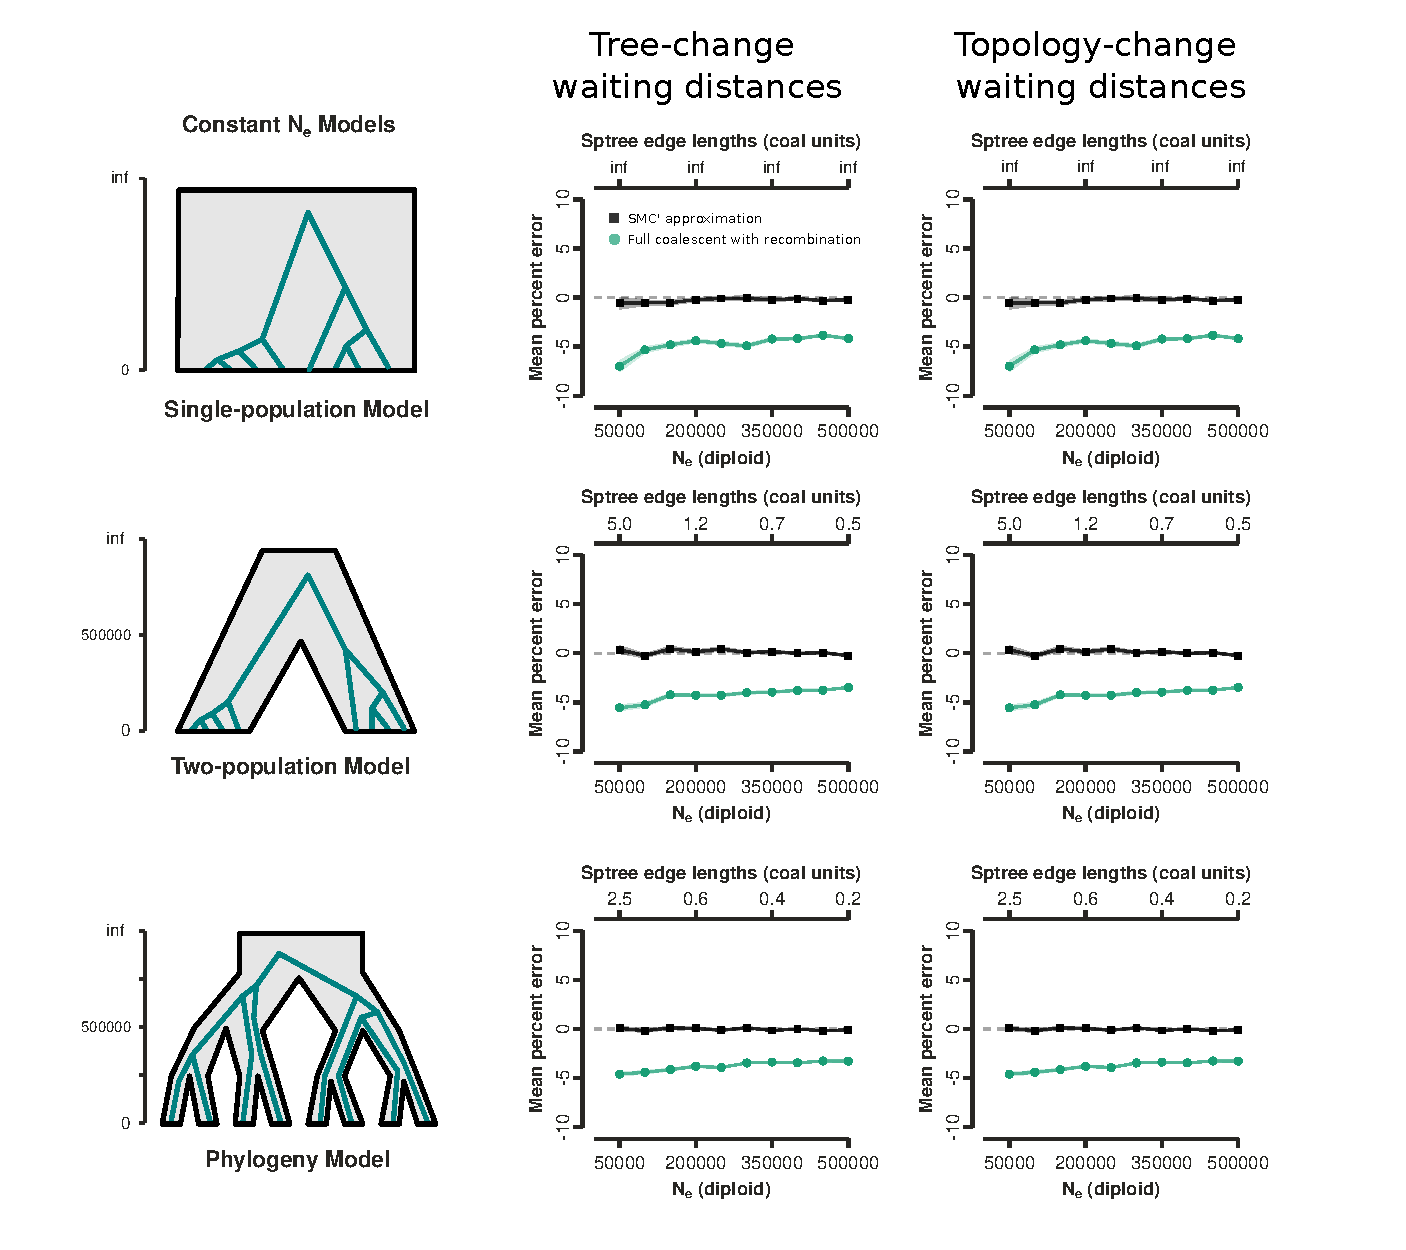
\includegraphics[width=0.99\textwidth]{figures/error-smc-approx.pdf}
	\caption{
		Error in MS-SMC' waiting distance expectations caused by the 
		SMC' approximation. Error was measured as the mean percent 
		difference between expected waiting distances calculated
		under the MS-SMC' and observed waiting distances in stochastic 
		coalescent simulations. Simulations were performed under either 
		the SMC' approximation (black) or the full coalescent 
		with recombination (green). The MS-SMC' tends to under-estimate 
		waiting distances compared to the full coalescent with recombination, 
		but shows only a slight bias at very low $N_e$ values compared to 
		simulations under the SMC'. 
		% The single-population model shows a more significant 
		% bias than either structured population model. This may be a consequence
		% of the greater variance in waiting distances in single	population models.
	}
     \label{fig:figS-bias-smc}
\end{figure}



\begin{figure}[p]
	\centering
	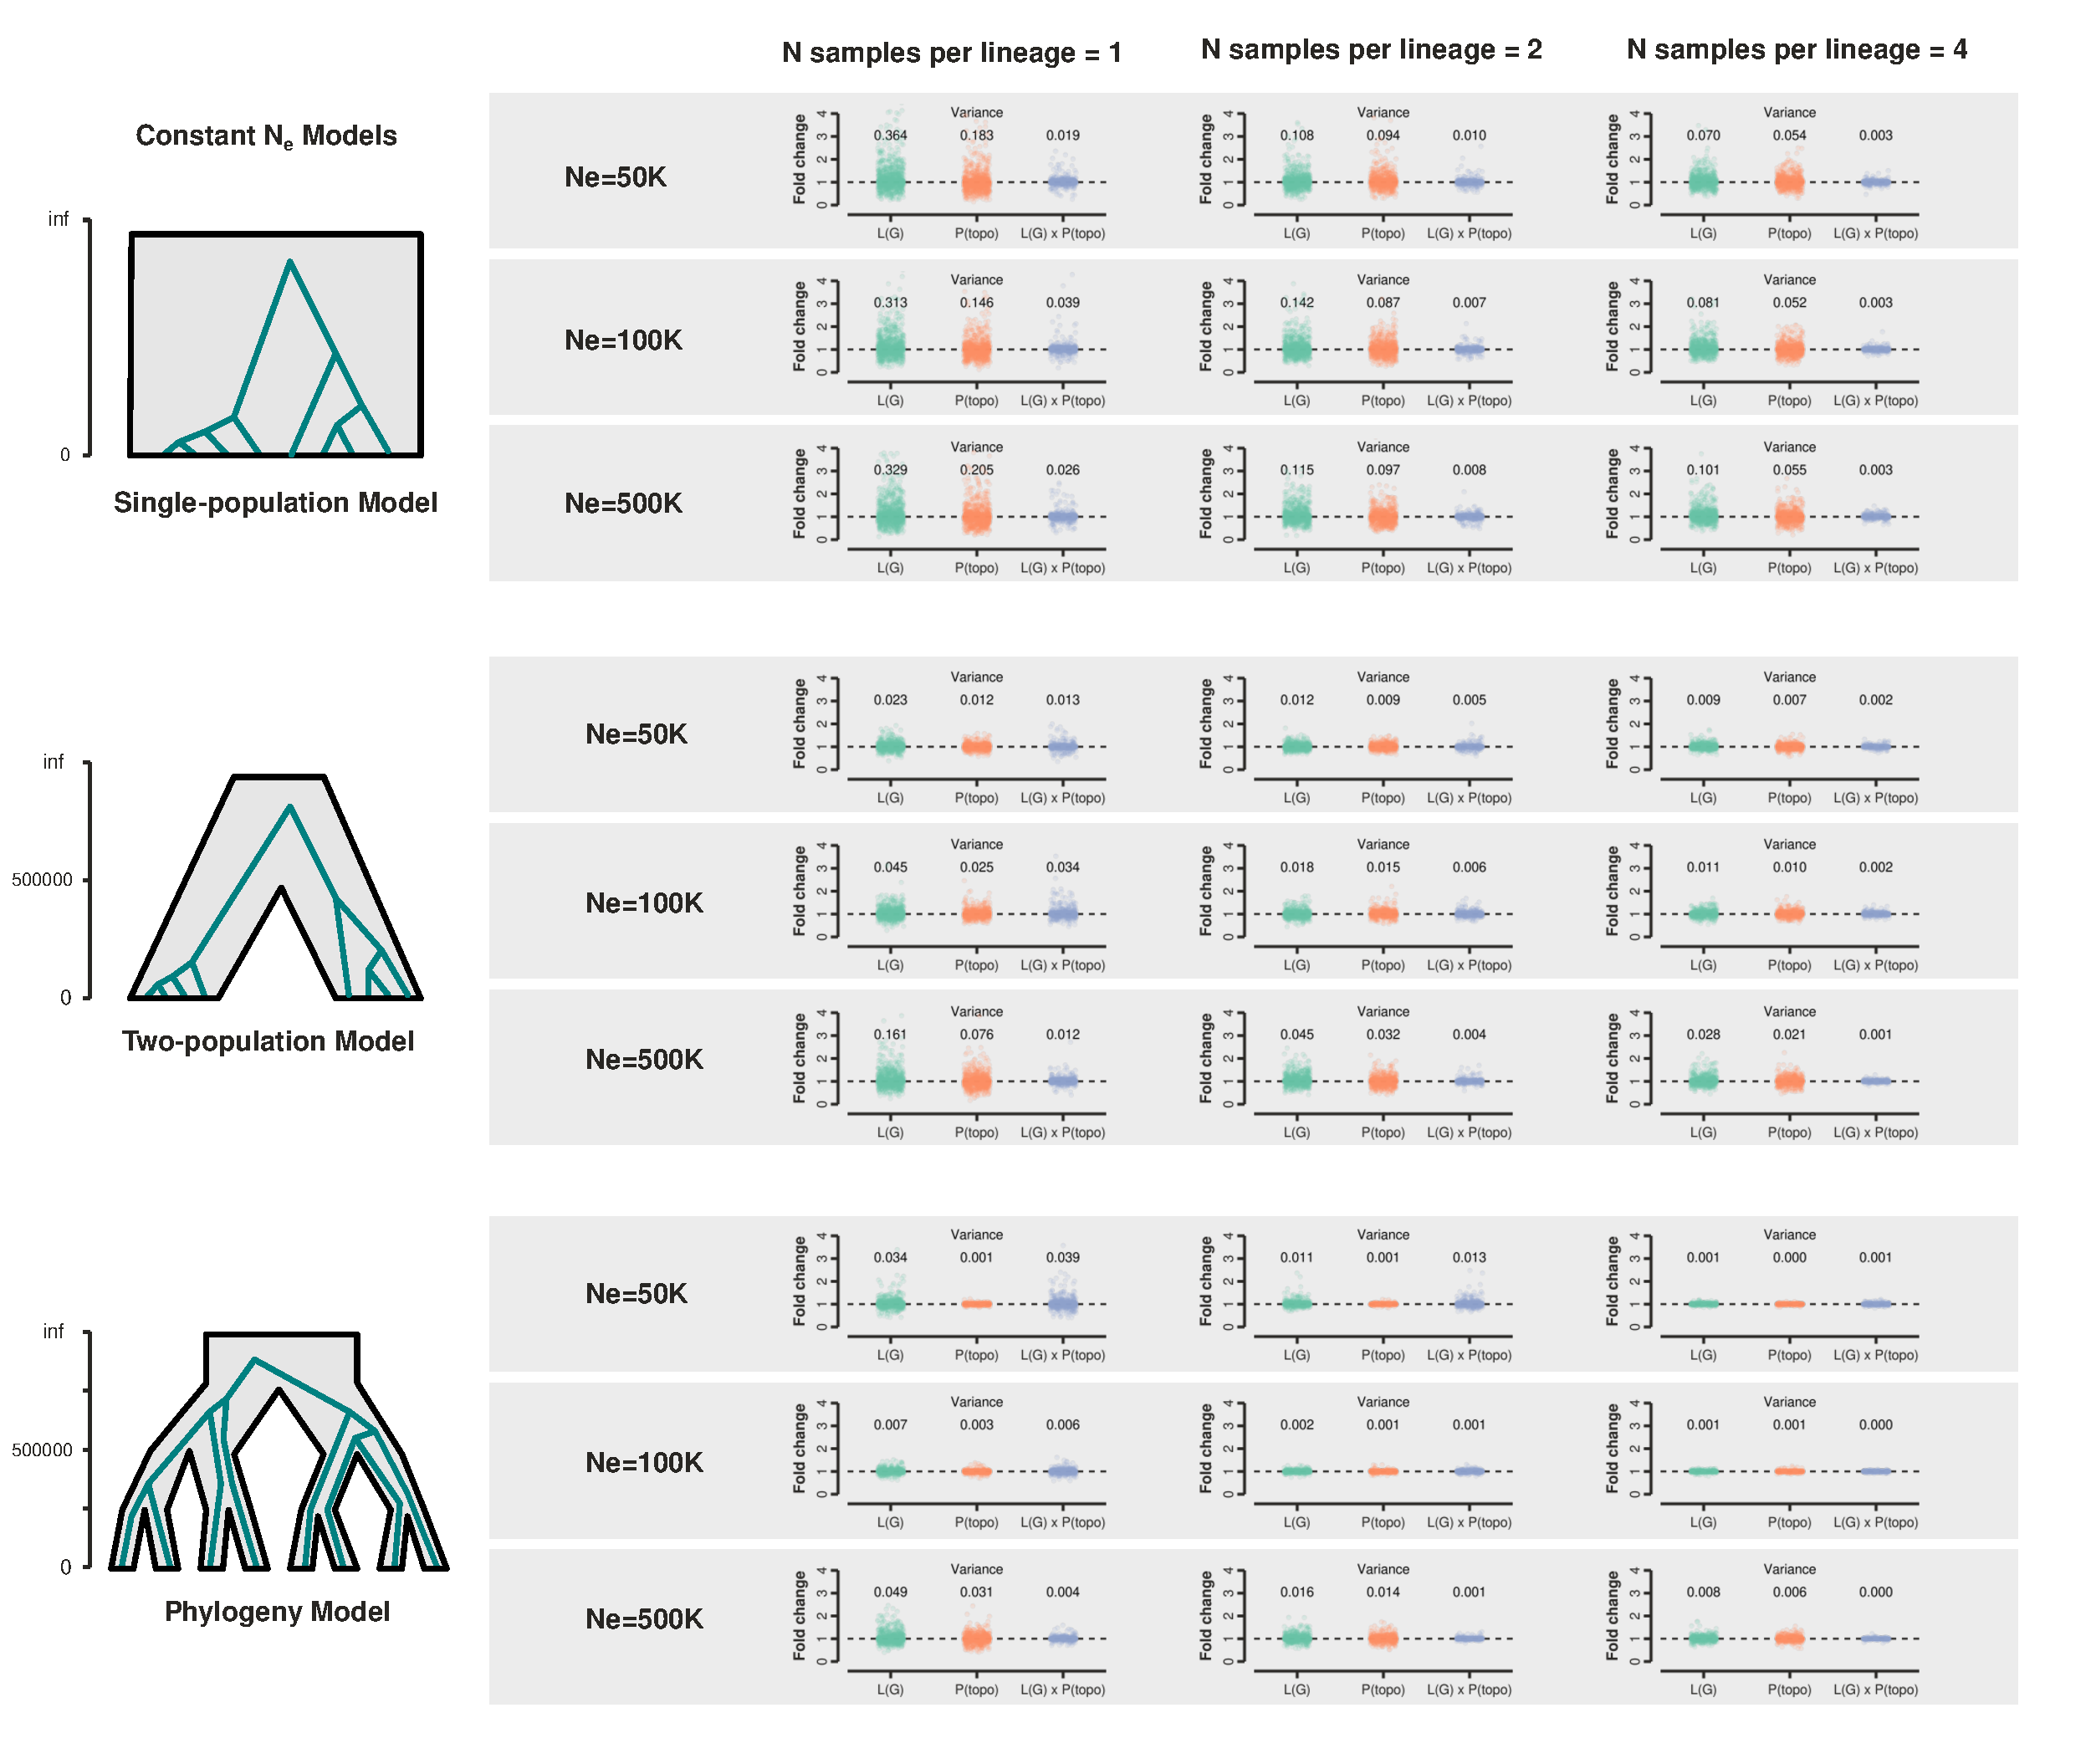
\includegraphics[width=0.99\textwidth]{figures/FigSX-bias.pdf}
	\caption{
		Variance in the fold-change in components affecting the expected waiting 
		distance to a topology change between the starting tree and a subsequent
		tree that has experienced a tree-change event that changed coalescent times
		but not the topology. The sum of genealogical edge lengths (L(G)), the 
		P(topology-change | S,G), and the product of these two terms are shown for
		three different demographic models and with different constant $N_e$ values, 
		and/or numbers of samples per lineage.
		When the fold-change in the product exhibits low variance around 1 the 
		MS-SMC' approximation for the expected waiting distance until a topology-change 
		is expected to be more accurate. Larger effective population sizes and 
		numbers of samples per lineage yield lower variance in the product.
	}
     \label{fig:figS-bias-topo}
\end{figure}


\section{Appendix: Derivations}

\subsection{Notation}

Information from the genealogy embedding table (described in the following paragraph) can be used 
in equations that 
calculate the 
probabilities of no-change, tree-change, and topology-change events under the 
MS-SMC'. These equations, described throughout rest of the Appendix, use the terms defined in 
Table~\ref{tab:table-notation}. 
% What is a species tree
A parameterized species tree, $\mathcal{S}$, is a multispecies coalescent 
model in which a set of isolated populations are related by a bifurcating
tree topology. Divergence times between lineages are in units of generations, 
and each edge (species tree interval) can be associated with a different constant 
diploid effective population size ($N_e$). 
A genealogy, $\mathcal{G}$, represents the genealogical relationships -- composing
a topology and coalescent times in units of generations -- for a set 
of sampled gene copies at some position in their genomes. A genealogy can be 
embedded in a species tree if the coalescent times between sampled gene copies
from different populations are not younger than a population divergence
event separating them.


\begin{table}[!b]
\centering
\caption{\label{tab:table-notation} 
	Summary of variables used in waiting distance equations. 
}
\begin{tabular}[t]{ |c|l| }
	\toprule
	Variable & Description \\
	\midrule
	$\mathcal{S}$    & An MSC model with topology, divergence times and effective population sizes. \\
	$\mathcal{G}$    & A genealogy that can be embedded in $\mathcal{S}$. \\
	$L(\mathcal{G})$ & Sum of edge lengths of genealogy $\mathcal{G}$. \\
	$b$ 			  & A focal branch in $\mathcal{G}$. \\
	$i$              & Interval in the genealogy embedding table in which recombination occurs.\\
	$\mathcal{I}_b$  & Ordered set of intervals on branch $b$.\\
	$\mathcal{I}_{c}$   & Ordered set of intervals on branch $c$, the parent of branch $b$.\\
	$\mathcal{I}_{bc}$  & Ordered union of sets $\mathcal{I}_{b}$ and $\mathcal{I}_{c}$.\\
	$\mathcal{J}_b(i)$  & Ordered set of intervals above $i$ on branch $b$.\\	
	$\mathcal{Q}_b(i,j)$ & Ordered set of intervals above $i$ and below $j$ on branch $b$.\\
	$\mathcal{K}(b,t)$ & Number of edges of $\mathcal{G}$ in the interval containing branch $b$ at time $t$.\\
	$k_x$              & Number of edges of $\mathcal{G}$ in interval $x$; piece-wise constant of $A(b,t)$.\\
	$\mathcal{N}(b,t)$ & Diploid effective population size in the interval containing branch $b$ at time $t$.\\
	$n_x$              & Diploid effective population size in interval $x$; piece-wise constant of $N(b,t)$. \\
	$t_r$		& Time of a recombination event, in generations. \\
	$\sigma_x$     & The lower boundary of interval $x$, in generations. \\
	$\mu_x$        & The upper boundary of interval $x$, in generations. \\	
	$d_x$          & The length of interval $x$, in generations. \\
	$t_b^l$        & The lower boundary of branch $b$, in generations. \\
	$t_b^u$        & The upper boundary of branch $b$, in generations. \\
	$t_b^m$        & The time at which a focal branch $b$ is able to coalesce with its sibling branch. \\
	% $m$            & Index of an interval in the genealogy embedding table with lower boundary $t_b^m$. \\
	$\mathcal{M}_b$  & Ordered set of intervals above $t_b^m$ on branch $b$.\\
	$\mathcal{L}_b$  & Ordered set of intervals below $t_b^m$ on branch $b$.\\	
	% $\mathcal{I}_b$  & The number of intervals containing branch $b$. \\
	\bottomrule
\end{tabular}
\end{table}



% each tip represents a sampled individual belonging to one of the species. The species tree 
% consists of a topology describing the history of population divergences, where each branch 
% of the topology has a constant effective diploid population size $N_b$ associated with it. 
% Within each branch, coalescence occurs at a constant per-generation rate of $\frac{1}{2N_b}$. 

% What is a genealogy, or set of genealogies, and what are samples
% One or more haploid genomes can be sampled from each lineage of a species tree.
% Each genome is composed of a mosaic of gene copies inherited from different ancestors,
% and thus the genealogy of 
% and at any position along the genome the relationships among the gene 

% distinguish between gene =copy and genomes.xs

Given a genealogy embedded in a species tree, a series of discrete
time intervals can be defined that are delimited 
by events that change the rate of coalescence. 
We refer to this 
set of discrete time intervals and their associated properties
as a genealogy embedding table (e.g., Table~\ref{tab:table-1}). 
In the waiting distance solutions for a single population with constant $N_e$ 
by \citet{deng_distribution_2021}, this table is delimited only by coalescent 
events, and the intervals are non-overlapping. 
Because $N_e$ is constant in their framework, only $k$ differs between 
intervals. Therefore, changes in $k$ alone determine differences in rates of coalescence, 
with $k$ decreasing monotonically in subsequent intervals from the tips towards the root. 
Our approach is similar, but adds additional complexity (Fig.~\ref{fig:fig1}). 
In the multispecies framework, genealogy embedding intervals are specific to each 
species tree branch, with each one corresponding to a time interval with a constant 
$k$ and $N_e$ in a specific species tree branch. 
Breakpoints between intervals arise where divergences 
occur in the species tree (increasing $k$ and potentially changing $N_e$) 
and where coalescent events occur in the genealogy (reducing $k$). 
Genealogy embedding intervals corresponding to different species tree 
branches can overlap in time.

Each branch on $\mathcal{G}$ will span one or more genealogy embedding 
intervals. The ordered set of intervals on a specific branch, $b$, is 
defined as $\mathcal{I}_b$. The lower and upper time bounding each interval is 
$\sigma_x$ and $\mu_x$, respectively, where $x$ is the index of the 
interval in the genealogy embedding table. The lower and upper bounds of
each branch are defined as $t_b^l$ and $t_b^u$, respectively. 
% Unlike in \citet{deng_distribution_2021}, where $N_e$ is constant, and $k$ 
% only decreases backwards in time, a multispecies scenario can see both 
% $k$ and $N_e$ increase or decrease through time as different 
% species tree intervals can have different $N_e$ values, and 
% \emph{species tree} coalescence events increase $k$, while 
% \emph{genealogy} coalescence events reduce $k$.


% For a selected branch $b$ on $\mathcal{G}$, intervals from the genealogy 
% embedding table corresponding to this branch can be indexed in order 
% ...\hl{update again}...
% from $\mathcal{I}_b-1$, where $\mathcal{I}_b$ is the total number of intervals
% in the branch. The times in generations marking the lower and upper bounds of each 
% branch $b$ are notated $t_l^b$ and $t_u^b$, respectively. Each interval of index $x$
% is bounded by times $\sigma_x$ and $\sigma_{x+1}$.

% We begin with a genealogical tree $\mathcal{G}$ sampled from the species tree according 
% to coalescent probabilities. This tree is embedded within the species tree so that the 
% time of coalescence for any two individuals from different species in $\mathcal{G}$ 
% is constrained to occur farther back in time than their species' coalescence times 
% in $\mathcal{S}$.


% Let $\mathcal{I}_b$ = (i$_1$, ..., i$_n$) be an ordered set of indices in the
% genealogy embedding table corresponding to intervals on branch $b$. These are
% indexed 


\subsection{Extending SMC' waiting distance solutions:}

% In \citet{deng_distribution_2021}, the genealogical tree was broken into a series of 
% intervals so that the number of remaining (not-coalesced) lineages was constant within
% each interval. In their method, the number of remaining lineages decreases monotonically
% through time from tipward to rootward intervals as lineages coalesce. Our approach is 
% similar, except that the intervals are branch-specific and correspond to intervals of 
% constant numbers of lineages to coalesce with ($A$) and constant effective population 
% size ($N$). Breakpoints may therefore exist where divergences occur in the species 
% tree (potentially changing both $A$ and $N$) and where coalescent events occur in 
% the genealogical tree (reducing $A$). Unlike in \citet{deng_distribution_2021}, $A$ 
% is no longer monotonic, since \emph{species} coalescent events can increase the number
% of lineages available for coalescence, while \emph{genealogical} coalescent events
% always reduce that number. 


% \subsection{The distribution of distances to any change in a genealogical tree}
% Our goal is to derive a distribution of waiting distances to the next tree change
% given a species tree and current genealogy.
% We begin with a genealogical tree $\mathcal{G}$ sampled from the species tree according 
% to coalescent probabilities. This tree is embedded within the species tree so that the 
% time of coalescence for any two individuals from different species in $\mathcal{G}$ is 
% constrained to occur farther back in time than their species' coalescence times in $\mathcal{S}$.

% We begin by assuming a specific branch and time of a recombination event. We then 
% integrate across possible times on that branch, and we sum across all branches on
% the tree to solve for the probability of the genealogy being unchanged given any 
% recombination event. Finally, we incorporate this probability into the exponential
% distribution presented in Equation 4.


% are each assigned an index increasing 
% from $0$ to $\mathcal{I}_b-1$, where $\mathcal{I}_b$ is 
% the total number of intervals in the branch. The times in generations marking the lower 
% and upper bounds of each branch $b$ are notated $t_l^b$ and $t_u^b$, 
% respectively. Each interval of index $x$ is bounded by times $\sigma_x$ and $\sigma_{x+1}$.

The probabilities of different recombination event types under the 
MS-SMC' are calculated from the probability that recombination occurs on 
a specific branch and the probabilities that the resulting detached 
subtree subsequently re-coalesces with any other available branch above that time. 
The opportunity for recombination to occur on a branch is scaled by 
its length in generations ($t_b^u$ - $t_b^l$). Similarly, the 
probability of re-coalescence on a branch is scaled by its length
and the coalescence rate. The latter can vary over the length of a branch
as it spans different intervals, and is a function of the effective 
population size in the species tree interval that includes branch $b$ at
a specified time, $\tau$, defined as $\mathcal{N}(b,\tau)$, and the number of 
other genealogy branches in the interval that includes branch $b$ at time $\tau$,
defined as $\mathcal{K}(b,\tau)$.
Finally, the probability that coalescence occurs over an interval of length ($t$) 
can be calculated from an exponential probability density $f(t; \lambda)$, 
where the rate parameter is $\lambda$ = $\frac{\mathcal{K}(b,\tau)}{2\mathcal{N}(b,\tau)}$, 
similar to equations 1-2. 
% or coalescence to occur on any branch
% coalescence events are calculated from the lengths of 
% intervals in units of generations, and the rate of coalescence within each
% interval, which is determined by the number of lineages that a given branch
% $b$ can coalesce with at any specified time $\mathcal{A}(b,\tau)$.

% \subsubsection{Probability of no-change or tree-change events}
\subsection{Probability of no-change}
\subsubsection{Given a branch and time of recombination}

The probability that a tree is unchanged by a recombination event -- meaning that 
no coalescent times are changed -- is the probability that the detached subtree 
re-coalesces with the same branch it detached from. Thus, we can integrate 
from the time of recombination ($t_r$) to the top of the branch ($t_b^u$) over the 
probability of sampling the same branch times the exponential probability density
of re-coalescing at any time on that branch above the time of recombination 
($\tau - t_r$). We take this integral with respect to $\tau$, where 
$\mathcal{K}(b,\tau)$ and $\mathcal{N}(b,\tau)$
can vary across the length of the branch if it spans different intervals.

% Where $A(\tau)$ is the number of lineages able to be coalesced with at any time $\tau$, 
% and $p(\tau|t_r)$ is the exponential probability density of coalescing any time 
% after the recombination event. 
% Thus, we are integrating over the probability
% of coalescence along the path of species tree intervals traversed
% by branch $b$, starting at the time of recombination and ending at the 
% end of the branch. If the branch spans only a single genealogy embedding 
% interval then $A(\tau)$ and $N(\tau)$... $\lambda$ = $\frac{A(b,\tau)}{2N(b,\tau)}$

% Through this series of one or more genealogy embedding intervals the 
% up to that time through the species tree intervals that are traversed
% by branch $b$, which can involve changing numbers of samples over time (A(t)), 
% and changing effective population sizes (N(t)).
% Here we define the coalescence rate at time $\tau$ as $\frac{A(\tau)}{N(\tau)}$. 
% Note that this differs from \citet{deng_distribution_2021}, 
% since our branch lengths are in units of generations rather than in
% coalescent units. 


% \begin{equation}
	% \mathbb{P}(\textrm{tree unchanged} | \mathcal{S}, \mathcal{G}, b, t_r) = 
	% \int_{t_r}^{t^u_b}\frac{1}{A(\tau)}p(\tau|t)d\tau
% \end{equation}	

% full equation
\begin{equation}
	\mathbb{P}(\textrm{tree-unchanged} | \mathcal{S}, \mathcal{G}, b, t_r) = 
	\int_{t_r}^{t_b^u} \frac{1}{\mathcal{K}(b,\tau)} f(\tau - t_r; \lambda) d\tau
\end{equation}

\noindent The exponential probability density function can be expanded, as in 
equation 2, where $\lambda$ is $\mathcal{K}(b,\tau)$ over 
2$\mathcal{N}(b,\tau)$:
% , where the probability of re-coalescence is the coalescent rate
% $\frac{1}{2N_e}$ times the number of samples $k$ that the detached subtree can
% reconnect with.
% number of samples
% the detached lineage can coalesce with over 2 times the diploid effective population
% size.
% . Here the rate parameter $\lambda$ is the probability that the
% detached lineage will re-coalesce with any of the other samples in the 
% interval at time $\tau$, which is $\frac{A(b,\tau)}{2N(b,\tau)}$. We can 
% substitute this into the exponential probability density function, and
% integrate over all time points above the recombination event:

% expand exponential probability function
\begin{equation}
	= \int_{t_r}^{t_b^u} 
	\frac{1}{\mathcal{K}(b,\tau)} 
	\frac{\mathcal{K}(b,\tau)}{2\mathcal{N}(b,\tau)}
	\exp \bigg\{
		-\int_{t_r}^{\tau} \frac{\mathcal{K}(b,s)}{2\mathcal{N}(b,s)}ds
		\bigg\} d\tau
\end{equation}

\noindent This simplifies to the following equation, which describes the probability that
the subtree re-coalesces at any time ($d\tau$) on $b$ above $t_r$, and 
that it does not re-coalesce at any intervening time ($ds$) between 
$t_r$ and $\tau$.

% cancel \mathcal{A}(t) 
\begin{equation}
	= \int_{t_r}^{t_b^u}
	\frac{1}{2\mathcal{N}(b,\tau)}
	\exp \bigg\{
		-\int_{t_r}^{\tau} \frac{\mathcal{K}(b,s)}{2\mathcal{N}(b,s)}ds
		\bigg\} d\tau
\end{equation}

\noindent Because the rate of re-coalescence is constant within each interval, 
we next split this equation into statements over each discrete interval that the
detached subtree could possibly re-coalesce with on branch $b$. (Recall, because
we are currently computing the probability of a no-change event we only need
to concern ourselves with re-coalescence on branch $b$.)
Here, the interval in which recombination occurred on branch $b$ is labeled
as $i$. 

In the equation below, the first integral describes the probability statement
over only part of interval $i$, from $t_r$ to $u_i$, rather than over its entire 
length, since re-coalescence can only occur above the time at which recombination 
occurred. By contrast, the latter parts of this equation are performed over the
entire lengths of each remaining interval above $i$, from the 
bottom ($\sigma_j$) to the top ($\mu_j$) of the interval.
The ordered set of all intervals above $i$ in $\mathcal{I}_b$ 
is defined as $\mathcal{J}_b(i) = \{j \in \mathcal{I}_b ~|~ j > i \}$. 

\begin{equation}
\begin{aligned}
	&= \int_{t_r}^{\mu_i}
		\frac{1}{2\mathcal{N}(b,\tau)} \exp 
			\bigg\{
				-\int_{t_r}^{\tau} \frac{\mathcal{K}(b,s)}{2\mathcal{N}(b,s)}ds
			\bigg\} d\tau + 
			% 
			\sum_{j \in \mathcal{J}_b(i)}
			\int_{\sigma_j}^{\mu_j}
			\frac{1}{2\mathcal{N}(\tau)} \exp 
			\bigg\{
				-\int_{t_r}^{\tau}
				\frac{\mathcal{K}(s)}{2\mathcal{N}(s)}ds
			\bigg\} d\tau\\
	% &~~where\\
	% &\mathcal{J}_b = \{j \in \mathcal{I}_b ~|~ j > i \}\\
\end{aligned}			
\end{equation}


% coalescence rate.

% \begin{equation}
% 	= \int_{t}^{t^u_b}\frac{1}{A(\tau)} \frac{A(\tau)}{N(\tau)}
% 	e^{-\int_t^\tau{}\frac{A(s)}{N(s)}ds} d\tau
% \end{equation}


% \begin{equation}
% 	= \int_{t}^{t^u_b}\frac{1}{N(\tau)}e^{-\int_t^\tau{}\frac{A(s)}{N(s)}ds} d\tau
% \end{equation}

% \subsubsection{Piece-wise constant probability of no-change}

% \begin{equation}
% 	= \int_{t_r}^{\sigma_{i+1}} 
% 		\frac{1}{2N(b,\tau)} \exp 
% 			\bigg\{
% 				-\int_{t_r}^{\tau} \frac{A(b,s)}{2N(b,s)}ds
% 			\bigg\} d\tau + 
% 			% 
% 			\sum_{j=i+1}^{\mathcal{I}_b-1}
% 			\int_{\sigma_{j}}^{\sigma_{j+1}}
% 			\frac{1}{2N(\tau)} \exp 
% 			\bigg\{
% 				-\int_{t_r}^{\tau}
% 				\frac{A(s)}{2N(s)}ds
% 			\bigg\} d\tau
% \end{equation}

% Once again, taking advantage of the piece-wise constant rate within each interval, 
\noindent We can now solve this equation and substitute constant values for 
$\mathcal{K}(b,\tau)$ and $\mathcal{N}(b,\tau)$ in each interval. 
Because the first term is computed over only part of the first interval we 
first solve this term separately, and then show the result for the later terms.
% \paragraph{First term --}
% \begin{equation}
	% = \frac{1}{a_i} - \frac{1}{a_i}e^{-\frac{a_i}{n_i}\sigma_{i+1}}e^{\frac{a_i}{n_i}t}
% \end{equation}
% \begin{equation}
% 	= \frac{1}{a_i} - 
% 	  {\color{red}\
% 		  \frac{1}{a_i}
% 		  \exp \bigg\{-\frac{a_i}{2n_i}\sigma_{i+1} \bigg\}
% 	  }
% 	  \exp \bigg\{\frac{a_i}{2n_i}t_r \bigg\}
% \end{equation}
The first term concerns the probability of re-coalescing in the same interval 
$i$ in which recombination occurred. The center part of this equation will 
appear again later, and so we define it as the function $f(i,i)$.

\begin{equation}
	= \frac{1}{k_i} - 
	  \frac{1}{k_i}
	  \exp \bigg\{-\frac{k_i}{2n_i} \mu_i \bigg\}
	  \exp \bigg\{\frac{k_i}{2n_i} t_r \bigg\}
\end{equation}

% \begin{equation}
	% = \frac{1}{a_i} +P_{ii}e^{\frac{a_i}{n_i}t}
% \end{equation}
\begin{equation}
	= \frac{1}{k_i} + f(i,i) \exp \bigg\{\frac{k_i}{2n_i} t_r \bigg\}
\end{equation}


% \paragraph{Later terms --}
\noindent We similarly define the function $f(i,j)$ for the later terms in 
this equation, which refer to the  
probability of re-coalescing in a later interval, $j$, than the one 
in which recombination occurred, $i$. This function requires also summing over 
any intervening intervals, $q$. For this, we define the function 
$\mathcal{Q}_b(i,j) = \{q \in \mathcal{I}_b ~|~ j > q > i\}$
to return the ordered set of intervals on branch $b$ between $i$ and $j$: 

% Once again, we can separate the part of this equation that is constant
% over intervals, and does not depend on the time of recombination $t_r$.
% Here this component, which we call $f(i,j)$, represents the probability 
% of re-coalescing in an interval above the one in which recombination 
% occurred.
% \begin{equation}
	% = \sum_{k=i+1}^{\mathcal{I}_b-1} e^{\frac{a_i}{n_i}t} \exp\left(-\frac{a_i}{n_i}\sigma_{i+1}-\sum_{q=i+1}^{k-1} \frac{a_q}{n_q}T_q\right)\left(\frac{1}{a_{k}}(1-e^{-\frac{a_{k}}{n_{k}}T_{k}})\right)
% \end{equation}

% \begin{equation}
% 	= \sum_{j=i+1}^{\mathcal{I}_b-1} 
% 	{\color{red}
% 	  \frac{1}{a_{j}}
% 	  \bigg(1 - \exp 
% 		  \bigg\{
% 			  -\frac{a_j}{2n_j} d_j 
% 		  \bigg\}
% 	  \bigg)
% 	  \exp \bigg\{
% 		  -\frac{a_i}{2n_i} \sigma_{i+1} - 
% 		  \sum_{q=i+1}^{j-1} 
% 		  \frac{a_q}{2n_q} d_q
% 		  \bigg\}
% 	}
% 	  \exp \bigg\{
% 		  \frac{a_i}{2n_i} t_r
% 		  \bigg\} 	  
% \end{equation}


\begin{equation}
\begin{aligned}
	&= \sum_{j \in \mathcal{J}_b(i)} 
	  \frac{1}{k_j}
	  \bigg(1 - \exp 
		  \bigg\{
			  -\frac{k_j}{2n_j} d_j 
		  \bigg\}
	  \bigg)
	  \exp \bigg\{
		  -\frac{k_i}{2n_i} \mu_i - 
		  \sum_{q \in \mathcal{Q}_b(i,j)}
		  \frac{k_q}{2n_q} d_q
		  \bigg\}
	  \exp \bigg\{
		  \frac{k_i}{2n_i} t_r
		  \bigg\}\\
     % &~~where\\
	% &\mathcal{Q}_b = \{q \in \mathcal{I}_b ~|~ j > q > i\}\\
\end{aligned}
\end{equation}



\begin{equation}
	= \sum_{j \in \mathcal{J}_b} 
	f(i,j)
	\exp \bigg\{ \frac{k_i}{2n_i} t_r \bigg\}
\end{equation}

% \begin{equation}
	% = \sum_{k=i+1}^{\mathcal{I}_b-1} e^{\frac{a_i}{n_i}t} P_{ik}
% \end{equation}

\noindent The $f(i,i)$ and $f(i,j)$ function above is represented in the main
text as equation 4. Adding the two terms that include these functions 
together we get equation 3 from the main text for the probability of a
no-change event given the timing and branch on which recombination occurs:

% $\mathbb{P}(\text{tree-unchanged} | \mathcal{S}, \mathcal{G}, b, t_r)$.

% PREVIOUS APPROVED EQUATION 3
\begin{equation}\tag{3}
\begin{aligned}
	&\mathbb{P}(\text{no-change} | \mathcal{S},\mathcal{G},b,t_r) = 
	\frac{1}{k_i} + f(i,i) \exp \bigg\{\frac{k_i}{2n_i} t_r\bigg\} +
	\sum_{j \in \mathcal{J}_b(i)} f(i,j) \exp\bigg\{\frac{k_i}{2n_i}t_r\bigg\} 
\end{aligned}
\end{equation}


% \begin{equation}
	% \mathbb{P}(\textrm{tree unchanged} | b,t,\mathcal{G},\mathcal{S}) = \frac{1}{a_i}+\sum_{k=i}^{\mathcal{I}_b-1}{P_{ik}e^{\frac{a_i}{n_i}t}}
% \end{equation}

\subsubsection{Across a full branch}
Having solved for the probability of the genealogy being unchanged given the 
time $t_r$ of the recombination event, our next step is to integrate this equation
across the entire branch with respect to $t_r$:

\begin{equation}
	\mathbb{P}(\text{tree-unchanged} | \mathcal{S}, \mathcal{G}, b) = 
		\frac{1}{t_b^u - t_b^l} 
		\int_{t_b^l}^{t_b^u} 
		\mathbb{P}(\text{tree-unchanged} | \mathcal{S}, \mathcal{G}, b, t_r) dt_r
\end{equation}

\noindent Plugging in the piece-wise constant solutions from equation 3
we get the following solution.

\begin{equation}
\begin{aligned}
	&= \frac{1}{t^u_b-t^l_b}
	\sum_{i \in \mathcal{I}_b}
	\frac{1}{k_i}d_i + 
	% 
	\bigg(
		\exp \bigg\{ \frac{k_i}{2n_i} \mu_{i} \bigg\}
		-\exp \bigg\{ \frac{k_i}{2n_i} \sigma_i	\bigg\}
	\bigg)\\
	% 
	&~~~~\Bigg[
		-\frac{2n_i}{k_i^2}
		\exp \bigg\{ -\frac{k_i}{2n_i} \mu_{i} \bigg\} + 
		% 
		\\
		&~~~~\frac{2n_i}{k_i}
		\Bigg(
			\sum_{j \in \mathcal{J}_b(i)}
			\exp \bigg\{
				-\frac{k_i}{2n_i} \mu_{i} -
				\sum_{q \in \mathcal{Q}_b(i,j)}
				\frac{k_q}{2n_q} d_q
				\bigg\}
			% \bigg)
			\frac{-1}{k_j} \exp \bigg\{-\frac{k_j}{2n_j} d_j \bigg\}
		\Bigg)
	\Bigg]
\end{aligned}
\end{equation}

\noindent Finally, this can be simplified to the following solution by expressing
the piecewise constant re-coalescence rates using the function $f(i,j$), as shown
in equation 5 from the main text.

\begin{equation*}
	\mathbb{P}(\textrm{tree-unchanged} | \mathcal{S},\mathcal{G},b) = 
	\frac{1}{t^u_b-t^l_b} \int_{t_b^l}^{t_b^u} 
	\mathbb{P}(\textrm{tree-unchanged} | \mathcal{S},\mathcal{G},b,t)dt
\end{equation*}

\begin{equation}\tag{5}
	= \frac{1}{t_b^u - t_b^l}
	\sum_{i \in \mathcal{I}_b} 
	\frac{1}{k_i} d_i + 
	\Bigg(
		\frac{2n_i}{k_i} 
		\sum_{j \in \mathcal{J}_b(i)} f(i,j)
		\bigg(
			\exp\bigg\{ \frac{k_i}{2n_i} \mu_i \bigg\} - 
			\exp\bigg\{ \frac{k_i}{2n_i} \sigma_i \bigg\}
		\bigg)
	\Bigg)
\end{equation}


\subsubsection{Across the whole tree}

At last, we can calculate the probability that, given a recombination event, 
the genealogy is unchanged. We do this by weighting each branch by its proportion 
of the total tree length and summing across the unchanging probabilities for 
all branches. This is equation 6 from the main text:

\begin{equation}\tag{6}
	\mathbb{P}(\textrm{tree-unchanged} | \mathcal{S}, \mathcal{G}) = 
	\sum_{b \in G}
	\bigg[
		\frac{t_b^u - t_b^l}{L(\mathcal{G})}
	\bigg]
	\mathbb{P}(\text{tree-unchanged} | \mathcal{S}, \mathcal{G}, b)
\end{equation}

\noindent We can then also derive the probability of a tree-change event
as $1-\mathbb{P}(\textrm{tree-unchanged} | \mathcal{S}, \mathcal{G})$.
% To derive the expected waiting distance to the next tree change, 
Following the approach described in equations 7-10, we can then calculate 
an exponential probability distribution for waiting distances between 
no-change or tree-change events using an exponential rate parameter that is
scaled by the probabilities of either recombination event type.
% expected waiting distance by treating this as an exponentially distributed
% random variable and calculating a rate parameter. 
% the value of  
% into the exponential distribution describing the waiting distance to the next 
% recombination event (introduced in Equation 4):
% \begin{equation}
% \begin{aligned}
% 	&p_r(d|\mathcal{G},\mathcal{S}) = 
% 	r\alpha_\mathcal{S}(\mathcal{G})L(\mathcal{G})\exp\left[-r\alpha_\mathcal{S}(\mathcal{G})L(\mathcal{G})d\right]\textrm{,} \\
% 	&~~where \\
% 	&\alpha_\mathcal{S}(\mathcal{G})=1-\mathbb{P}(\textrm{tree unchanged} | \mathcal{G},\mathcal{S}).
% \end{aligned}
% \end{equation}


\subsection{Probability of topology change}
Next, we derive the probability of a topology-unchanged event, from which
we can get the associated probability of a topology-change event. 
As in the first section, we first derive a solution given an individual 
branch and time of recombination. We then extend this solution to an entire branch, and we 
finally sum across branches to get a probability for the entire genealogy. 
To isolate events that do not cause a topology change, we must find
the union of events that cause a no-change event in addition to two types of 
possible tree-change events which affect only branch lengths but not the 
topology. These two types of events correspond to a re-coalescence with the 
sibling to branch $b$, termed $b'$, or with its parent, $c$ (Fig.~\ref{fig:fig3}d).
Because branch $c$ is always ancestral to $b$, a recombination
event on $b$ can potentially re-coalesce anywhere on $c$; however, 
this is not the case for $b'$, which may only exist or be available for 
re-coalescence over part of the length of $b$. It is therefore important 
to define the lowest time point at which re-coalescence with $b'$ is 
possible, termed $t_b^m$. 

In the single population model of \citet{deng_distribution_2021}, 
$t_b^m$ occurs at the maximum value of $t_b^l$ and $t_{b'}^l$, 
representing the lower bounds of $b$ and $b'$, respectively. 
In our MSC-based model we must also incorporate potential 
constraints imposed by population barriers, and so $t_b^m$ occurs at 
the maximum of $t_b^l$, $t_{b'}^l$, and any population divergence 
events that separate $b$ and $b'$ (Fig.~\ref{fig:figS-tbm}a-c).


\begin{figure}[t]
	\centering
	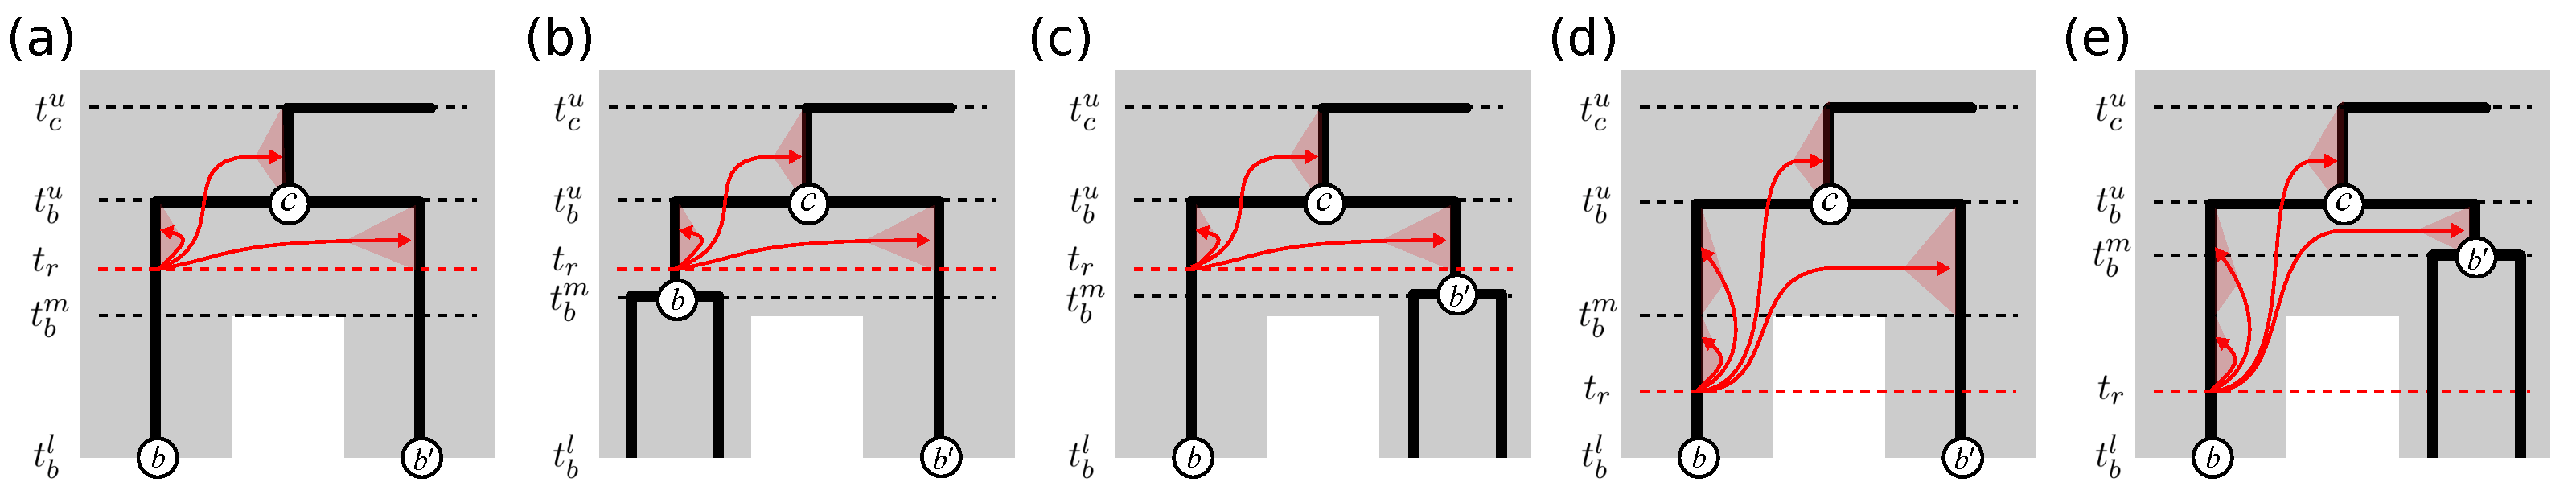
\includegraphics[width=0.95\textwidth]{figures/FigS-tbm.pdf}
	\caption{
		To calculate the probability that recombination on genealogy branch 
		$b$ leads to a topology change involves summing over the probabilities 
		that the detached lineage does not re-coalesce with either
		itself, its sibling, or its parent ($b$, $b'$ or $c$, respectively). 
		When the timing of recombination ($t_r$) occ...
		$b$ and $b'$ can either exist 
		in different species tree intervals (a) or the same interval (b). This 
		restricts the probability of tree-change outcomes (e.g., shortened coalescent 
		time) until the lowest shared interval between $b$ and $b'$ at time 
		$t_m$. This leads to two ordered sets of intervals (c-d) used in 
		equations 11 and 12.
	}
	\label{fig:figS-tbm}
\end{figure}

% of categories 2 and 3, which just change branch lengths, to isolate the probability
% that a recombination event changes the \emph{topology} of the tree.
% We also designate the timepoint $t_b^m$, which we use to 
% break the problem into two cases. While the single-population example in 
% \citet{deng_distribution_2021} uses $t_{b'}^l$ as this breakpoint, the species tree 
% introduces more complexity, and we instead use the maximum of three values: 
% $t_{b'}^l$, $t_{b}^l$, and $t_{(b,b')}^w$, which we define as the merging time 
% for the species tree branches separating $b$ and $b'$ (Figure-supplement).

\subsubsection{Given a branch and time of recombination}
Using the definition for $t_b^m$ from above, we can describe the probability
of a topology-unchanged event given the branch and time of recombination
as a two-part solution. These two parts correspond to scenarios in which
the time of recombination, $t_r$, occurs either above (Fig.~\ref{fig:figS-tbm}a-c)
or below (Fig.~\ref{fig:figS-tbm}d-e) $t_b^m$. When $t_r$ $<=$ $t_b^m$, there
are only two distinct intervals over which re-coalescence can occur: from
$t_r$ to $t_b^u$ on branches $b$ or $b'$, and from $t_b^u$ to $t_c^u$ on 
branch $c$ (Fig.~\ref{fig:figS-tbm}a-c). By contrast, when $t_r$ $>$ $t_b^m$
there are three distinct intervals for re-coalescence: from $t_r$ to $t_b^m$
on $b$, $t_b^m$ to $t_b^u$ on $b'$, and $t_b^u$ to $t_c^u$ on 
branch $c$ (Fig.~\ref{fig:figS-tbm}d-e). Thus, in the first scenario 
the opportunity for re-coalescence is the same for branches $b$ 
and $b'$, whereas in the latter scenario it is different.

% isn't the tr < tbm part redundant with the next part?
% \hl{In the first case} (Fig.~\ref{fig:fig3}a), where $t_r$ $<$ $t_b^m$ and 
% $t_r \in [\sigma_i, \sigma_{i+1}] \subset [t_b^l,t_b^m]$
% it is necessary to integrate over coalescence probabilities in three distinct 
% sections: from $t_r$ to $t_b^m$, $t_b^m$ to $t_b^u$, and $t_b^u$ to $t_c^u$. 
% (Note, these sections may be composed of multiple genealogy embedding 
% intervals if they contain additional species divergence events).
% The first section is notable for representing the core
% difference between this first case and the second case below. 
% When a recombination event occurs in the first section on $b$ there is a span 
% from $t_r$ to $t_b^m$ where $b$ can re-coalescence with itself but not yet 
% with $b'$, since at least one species divergence event separates them.
% Thus, although re-coalescence can occur in this span of time, it cannot lead to 
% changes in the genealogy. 
% In the second section, 
% $b$ can re-coalesce with $b$ or $b'$, leading to either no change or a tree 
% change (shortened coalesence time). Finally, in the third section $b$ can 
% only re-coalesce with $c$, leading to a tree change that lengthens $b$'s 
% coalescence time. 
% An integration over the probabilities of each allowable 
% event on branch $b$ over all three distinct sections leads to the first
% probability statement below. 
% In the second case (Fig.~\ref{fig:fig3}b), where $t_r$ $>$ $t_b^m$ and 
% $t_r \in [\sigma_i, \sigma_{i+1}] \subset [t_b^m,t_b^u]$, 
% it is only necessary to integrate over probabilities across a subset of the 
% second section, and across the entire third section described above, leading
% to the second statement below:

Retaining the correct order of intervals is important in these calculations, 
particularly for $f(i,j)$, which involves summing over not only the information
in the $i$ and $j$ intervals, but also all of the intervals that lie between 
them. To iterate over ordered intervals on each branch we define additional
indexing variables. Just as $\mathcal{I}_b$ defines the ordered set of intervals 
on branch $b$, $\mathcal{I}_c$ is the ordered set of intervals on branch $c$, and
$\mathcal{I}_{bc}$ is the ordered union of these sets. In addition, we define
$\mathcal{M}_{b}$ as the ordered intervals on branch $b$ above 
$t_b^m$, and $\mathcal{L}_{b}$ as the ordered intervals on branch $b$ 
below $t_b^m$.
We can now derive a probability for the two distinct scenarios:

% As in \citet{deng_distribution_2021}, we break the problem into two cases: a first case in 
% which $t$ belongs to the interval from the base of the focal branch to $t^m_b$, and a second 
% case in which $t$ belongs to the interval from $t^m_b$ to $t^u_b$. 

% We define $bc$ as the ordered union of the sets of intervals on 
% branches $b$ and $c$ (Fig.~\ref{fig:fig3}c), such that $\mathcal{I}_{bc}$ is 
% the summed number of intervals in this set.
% % that can be used to index ordered intervals in this set.
% Similarly, we define the intersection of the sets of intervals in $b$
% and $b'$ as $bb'$, which includes only intervals in which both of 
% these branches occur (i.e., it excludes intervals where they
% are embedded in separate species tree branches). Finally, we 
% define $m$ as the index of the lowest interval in $bb'$ 
% (occurring at time $t_b^m$) where both $b$ and $b'$ occur. 


%%%%%%%%%%%%%%%%%%%%%% I'm not sure we need this figure anymore, can use maintext fig3.
% \begin{figure}[t]
% 	\centering
% 	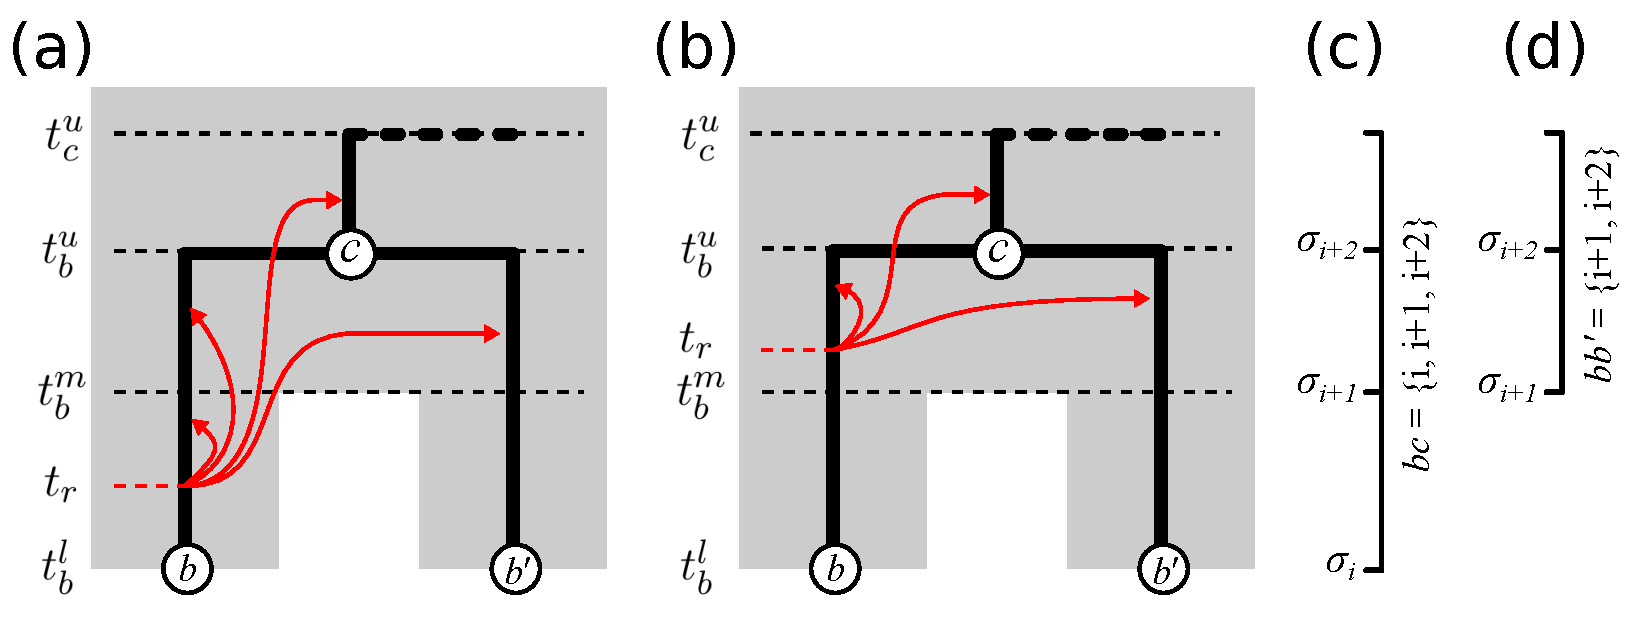
\includegraphics[width=0.75\textwidth]{figures/FigS1-sibling-parent-it2.pdf}
% 	\caption{
% 		To calculate the probability that recombination on a genealogy branch
% 		($b$) leads to a topology change involves summing over the probabilities 
% 		that a detached lineage does not re-coalesce with either
% 		itself ($b$), its sibling ($b'$) or its parent ($c$) branches. At the time 
% 		recombination occurs ($t_r$) the branches $b$ and $b'$ can either exist 
% 		in different species tree intervals (a) or the same interval (b). This 
% 		restricts the probability of tree-change outcomes (e.g., shortened coalescent 
% 		time) until the lowest shared interval between $b$ and $b'$ at time 
% 		$t_m$. This leads to two ordered sets of intervals (c-d) used in 
% 		equations 11 and 12.
% 	}
% 	\label{fig:figSSS}
% \end{figure}



\paragraph{First case --} Given $t_r$ $<$ $t_b^m$, we integrate over the three
distinct intervals where re-coalescence can occur. The first is unique to branch $b$, 
the second integral is multiplied by two since from $t_b^m$ to $t_b^u$ re-coalescence
can occur with $b$ or $b'$, and the final integral is over the length of branch $c$.
By substituting the piece-wise constant solutions for each interval into this equation
it can simplifed to the final form below, also shown in equation 11 of the main text:

\begin{equation}
\begin{aligned}
	&\mathbb{P}(\text{topology-unchanged} | \mathcal{S}, \mathcal{G}, b, t_r) \\
	&= \int_{t_r}^{t_b^m}
	\frac{1}{\mathcal{K}(b,\tau)} f(\tau - t_r; \lambda) d\tau + 
	\int_{t_b^m}^{t_b^u}
	\frac{2}{\mathcal{K}(b,\tau)} f(\tau - t_r; \lambda) d\tau + 
	\int_{t_b^u}^{t_c^u} \frac{1}{\mathcal{K}(b,\tau)} f(\tau - t_r; \lambda) d\tau \\
	&= \frac{1}{k_i} + 
	\sum_{j \in \mathcal{I}_{bc}}	f(i,j) \exp \bigg\{	\frac{k_i}{2n_i} t_r \bigg\} + 
	\sum_{j \in \mathcal{M}_b}    f(i,j) \exp \bigg\{ \frac{k_i}{2n_i} t_r \bigg\}
\end{aligned}
\end{equation}

\paragraph{Second case --} Given $t_r$ $>=$ $t_b^m$, we only need to integrate over
two distinct intervals, thus we simply drop the first term from the equation above.
The final form of this equation is also shown in equation 11 of the main text:

\begin{equation}
\begin{aligned}
	&\mathbb{P}(\text{topology-unchanged} | \mathcal{S}, \mathcal{G}, b, t_r) \\
	&= \int_{t_r}^{t_b^u} \frac{2}{\mathcal{K}(b,\tau)} f(\tau - t_r; \lambda) d\tau + 
	 \int_{t_b^u}^{t_c^u} \frac{1}{\mathcal{K}(b, \tau)} f(\tau - t_r; \lambda) d\tau \\
	&= 2 \bigg(
		\frac{1}{k_i} + 
		\sum_{j \in \mathcal{I}_b} f(i,j) \exp \bigg\{ \frac{k_i}{2n_i} t_r \bigg\}
	\bigg) + 
	\sum_{j \in \mathcal{I}_c} f(i,j) \exp \bigg\{ \frac{k_i}{2n_i} t_r \bigg\}
\end{aligned}
\end{equation}

\subsubsection{Across a full branch}

Now we derive the overall probability that a recombination event falling on a specific branch will 
change the topology by integrating across the range of possible values for $t_r$.
Following the approach above, we split this problem into two parts, above and below
$t_b^m$, and we sum the two cases.

\begin{equation}
	\mathbb{P}(\text{topology-unchanged} | \mathcal{S}, \mathcal{G}, b) = 
	\frac{1}{t_b^u - t_b^l} \int_{t_b^l}^{t_b^u}
	\mathbb{P}(\text{topology-unchanged} | \mathcal{S}, \mathcal{G},b, t_r) dt_r
\end{equation}

\begin{equation}
	= \frac{1}{t_b^u - t_b^l}
	\bigg[
		\bigg(
			\int_{t_b^l}^{t_b^m} + 
			\int_{t_b^m}^{t_b^u}
		\bigg)
		\mathbb{P}(\text{topology-unchanged} | \mathcal{S}, \mathcal{G},b, t_r) dt_r
	\bigg]
\end{equation}


\paragraph{First case --}
We can simply sum over each entire interval below $t_b^m$ where $t_r$ could occur, and 
substitute piece-wise constant solutions for the probabilities that a detached
subtree will re-coalesce over the subset of targeted intervals above this that
do not cause a topology-change.

\begin{equation}
\begin{aligned}
	&\int_{t_b^l}^{t_b^m} {\mathbb{P}(\text{topology-unchanged} | \mathcal{S}, \mathcal{G}, b, t_r)} dt_r \\
	&= \sum_{i \in \mathcal{L}_b} \frac{1}{k_i} \Bigg[ 
		d_i + 2n_i \bigg( 
			\exp \bigg\{\frac{k_i}{2n_i} \mu_i \bigg\} - 
			\exp \bigg\{\frac{k_i}{2n_i} \sigma_i\bigg\} 
		\bigg)
		\bigg(
			\sum_{j \in \mathcal{I}_{bc}} f(i,j) + \sum_{j \in \mathcal{M}_b} f(i,j) 
		\bigg) 
	\Bigg]
\end{aligned}
\end{equation}

\paragraph{Second case --}
Similarly, we can sum over each entire interval above $t_b^m$ (up to $t_b^u$) and substitute piece-wise
constant solutions for the same selected subset of intervals:

\begin{equation}
\begin{aligned}
	&\int_{t_b^m}^{t_b^u} \mathbb{P} (\textrm{topology-unchanged} | \mathcal{S}, \mathcal{G}, b, t_r) dt_r \\
	&= \sum_{i \in \mathcal{M}_b} \frac{1}{k_i} \Bigg[ 
		2d_i + 2n_i \bigg( 
			\exp \bigg\{ \frac{k_i}{2n_i} \mu_i \bigg\} - 
			\exp \bigg\{ \frac{k_i}{2n_i} \sigma_i \bigg\}
		\bigg) 
		\bigg(2 \sum_{j \in \mathcal{I}_b} f(i,j) + \sum_{j \in \mathcal{I}_c} f(i,j) \bigg)
	\Bigg]
\end{aligned}
\end{equation}

\paragraph{Result --}
If we express the inner summed terms from the equations above, composed of piece-wise
constant values from their intervals, as $p_{b,1}^{(i)}$ and $p_{b,2}^{(i)}$, 
respectively, then the final solution can be expressed more concisely. 
This is shown in the main text as equation 12.

\begin{equation}\tag{12}
     \mathbb{P}(\text{topology-unchanged} | \mathcal{S}, \mathcal{G}, b) = 
     \frac{1}{t_b^u - t_b^l} 
     \bigg[ 
	    \sum_{i \in \mathcal{L}_b} p_{b,1}^{(i)} + 
	    \sum_{i \in \mathcal{M}_b} p_{b,2}^{(i)}
	\bigg]
\end{equation}


\subsubsection{Across the whole tree}

Finally, we sum across all branches, each weighted by their relative length, 
to find the probability of a recombination event changing the 
topology of the tree. This appears as equation 13 in the main text.

\begin{equation}\tag{13}
\begin{aligned}
    &\mathbb{P}(\text{topology-unchanged}| \mathcal{S}, \mathcal{G}) = 
    \sum_{b \in \mathcal{G}}
    \frac{t_b^u - t_b^l}
    {L(\mathcal{G})} \times \mathbb{P}(\text{topology-unchanged}| \mathcal{S}, \mathcal{G}, b) \\
    % 
    & = \frac{1}{L(\mathcal{G})} \sum_{b \in \mathcal{G}}
     \bigg[ 
	    \sum_{i \in \mathcal{L}_b} p_{b,1}^{(i)} + 
	    \sum_{i \in \mathcal{M}_b} p_{b,2}^{(i)}
	\bigg]
\end{aligned}
\end{equation}


\subsubsection{Examples}
Examples showing how to compute the probablity of a no-change (tree-unchanged) 
or topology-change event are shown with didactic step-by-step instructions in 
Fig.~\ref{fig:figS-tree-equations} and Fig.~\ref{fig:figS-topo-equations}, 
respectively.

\begin{figure}[p]
	\centering
	\includegraphics[width=0.95\textwidth]{figures/verbose-equations}
	\caption{A step-by-step calculation of the probability of a tree-unchanged 
	event under the MS-SMC' given a species tree and genealogy.
	}
	\label{fig:figS-tree-equations}
\end{figure}




\begin{figure}[p]
	\centering
	\includegraphics[width=0.95\textwidth]{figures/verbose-equations-topology}
	\caption{A step-by-step calculation of the probability of a topology-unchanged 
	event under the MS-SMC' given a species tree and genealogy.
	}
	\label{fig:figS-topo-equations}
\end{figure}



% \begin{figure}[t]
% 	\centering
% 	%\fbox{\rule[-.5cm]{4cm}{4cm} \rule[-.5cm]{4cm}{0cm}}
% 	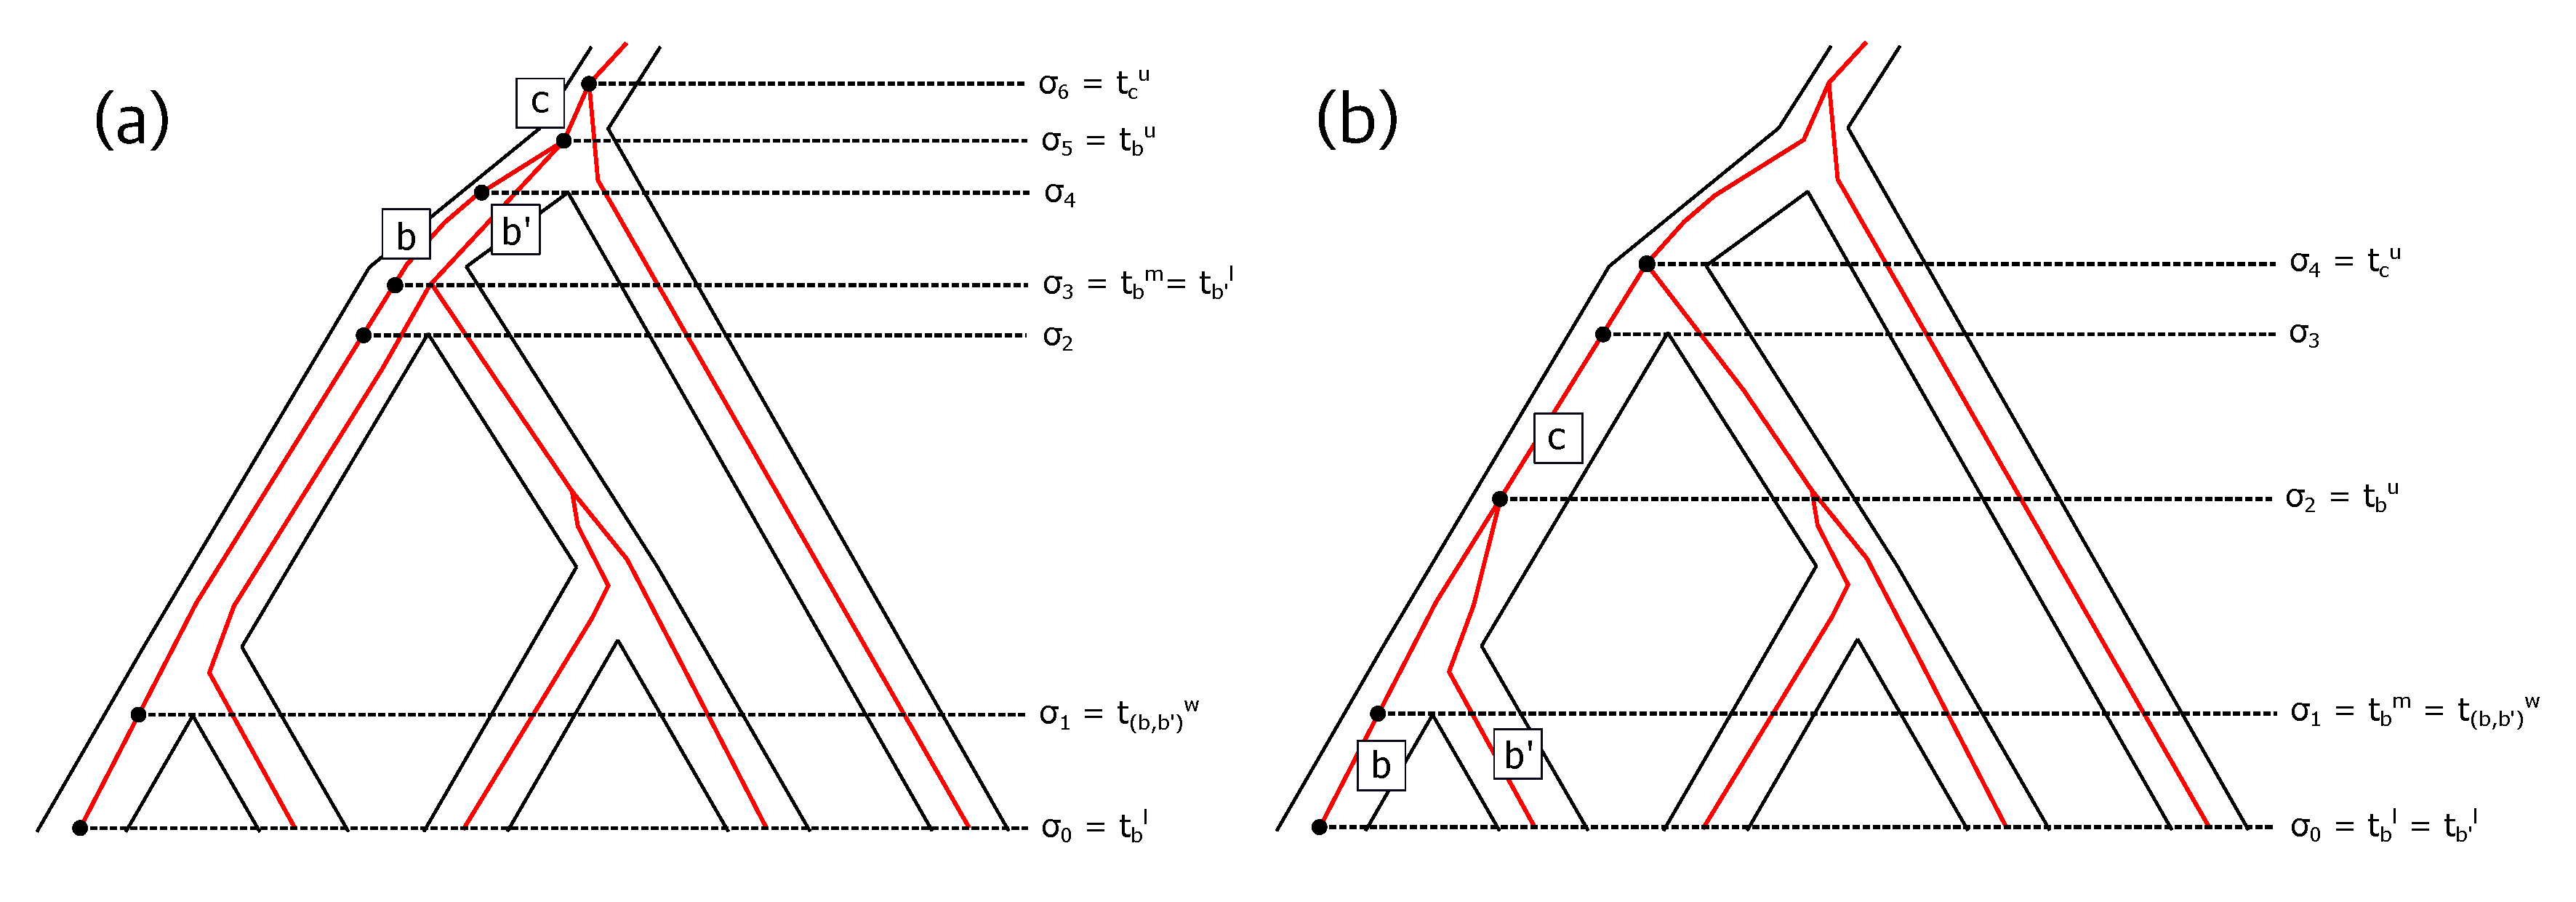
\includegraphics[width=0.9\textwidth]{figures/FigS1-topology_illustration.pdf}
% 	\caption{Illustrating the parameters for calculating the distribution of distances 
% 	to a change in the topology of a genealogy. Panels (a) and (b) show slightly 
% 	different genealogies embedded in the same species tree. In both (a) and (b), 
% 	the focal branch $b$ is the one leading from the left-most species. 
% 	Branches $c$ and $b'$ -- the parent and sibling branches, respectively -- are 
% 	also both labeled. Note that in (a), $t_b^m$ corresponds to $\sigma_3$, while
% 	in (b) it corresponds to $\sigma_1$.}
% 	% \label{fig:fig5}
% \end{figure}


%%%%%%%%%%%%%%%%%%%%%%% This table doesn't seem necessary.
% \begin{table}[h]
% \centering
% \caption{\label{tab:table-S1} 
% 	A table summarizing the relationships among branches in the genealogical tree embedded in the species tree in Figure 1. 
% }
% \begin{tabular}[t]{ |c|c|c|c|c|c|c| }
% 	\toprule
% 	Branch & $\mathcal{I}_b$ & $t_b^l$ & $t_b^u$ & Parent & Sibling & $t_b^m$ \\
% 	\midrule
% 	0  &  1 & 0      & $t_7$  & 7  & 1  & 0          \\
% 	1  &  1 & 0      & $t_7$  & 7  & 0  & 0          \\
% 	2  &  3 & 0      & $t_9$  & 9  & 8  & $W_{AB}$   \\
% 	3  &  1 & 0      & $t_8$  & 8  & 4  & 0          \\
% 	4  &  1 & 0      & $t_8$  & 8  & 3  & 0          \\
% 	5  &  4 & 0      & $t_{11}$ & 11 & 6  & $W_{ABCD}$ \\
% 	6  &  2 & 0      & $t_{11}$ & 11 & 5  & $W_{ABCD}$ \\
% 	7  &  4 & $t_7$  & $t_{10}$ & 10 & 9  & $t_9$      \\
% 	8  &  2 & $t_8$  & $t_9$  & 9  & 2  & $W_{AB}$   \\
% 	9  &  2 & $t_9$  & $t_{10}$ & 10 & 7  & $t_9$      \\
% 	10 &  3 & $t_{10}$ & $t_{12}$ & 12 & 11 & $t_{11}$     \\
% 	11 &  1 & $t_{11}$ & $t_{12}$ & 12 & 10 & $t_{11}$     \\
% 	\bottomrule
% \end{tabular}
% \end{table}





\end{document}
